\documentclass[11pt]{article}
 
\usepackage[top=0.75in, bottom=1.25in, left=1in, right=1in]{geometry} 
\usepackage{amsmath,amsthm,amssymb}
\usepackage{mathtools}
\usepackage{tikz}
\usepackage{tikz-cd}
\usetikzlibrary{decorations.pathmorphing}
\usepackage{graphicx}
\usepackage{fancybox}
\usepackage{fancyref}
\usepackage{hyperref}
\usepackage{enumitem}
\usepackage{afterpage}
%\usepackage{extarrows}
\usepackage{fancyhdr}
\usepackage{datetime}
\usepackage{array}
\usepackage{mathrsfs}
\usepackage{titlesec}
\usepackage{slashbox}
%\usepackage{relsize}
\usepackage{mdframed}
\usepackage[overload]{empheq}
%\usepackage[notref,notcite]{showkeys}
\usepackage{xcolor}
\definecolor{firebrick}{RGB}{178,34,34}
\definecolor{teal}{RGB}{0,128,128}
\definecolor{indigo}{RGB}{75,0,130}
\definecolor{darkblue}{rgb}{0.0,0.0,.7}
\definecolor{lightgrey}{RGB}{212, 212, 212}
%\usepackage{eulervm}
%\usepackage{mnsymbol}
\usepackage{scalerel}
\setcounter{MaxMatrixCols}{20}
%\usepackage{bbm}
\usepackage{mathpazo}
%\usepackage{newtxmath}
\usepackage[T1]{fontenc}
\usepackage[cal = pxtx, scr = boondox]{mathalpha}

\AtBeginDocument{
  \DeclareSymbolFont{AMSb}{U}{msb}{m}{n}
  \DeclareSymbolFontAlphabet{\mathbb}{AMSb}}
  
\DeclareMathAlphabet{\mathbx}{U}{BOONDOX-ds}{m}{n}
\SetMathAlphabet{\mathbx}{bold}{U}{BOONDOX-ds}{b}{n}
\DeclareMathAlphabet{\mathbbx} {U}{BOONDOX-ds}{b}{n}
  
\tikzset{
    labl/.style={anchor=north, rotate=90, inner sep=.5mm}
}

\def\shortyear#1{\expandafter\shortyearhelper#1}
\def\shortyearhelper#1#2#3#4{#3#4}

\newdateformat{shortmonth}{%
  \shortmonthname[\THEMONTH]}
\newdateformat{monthyeardate}{%
  \monthname[\THEMONTH] \THEYEAR}

\pagestyle{fancy}
\renewcommand{\headrulewidth}{0pt}
\fancyhf{}
\cfoot{{\footnotesize {\color{black} \thepage}}}
\lfoot{{\footnotesize {\color{gray} Bhamidipati}}}
%\lfoot{{\footnotesize {\color{gray} Bhamidipati, \shortmonth\today\ '\shortyear{\the\year}}}}
\rfoot{{\footnotesize {\color{gray} MATH 110 | Fall 2021}}}

%Here are some user-defined notations
\newcommand{\zz}{\mathbb Z}   %blackboard bold Z
\newcommand{\qq}{\mathbb Q}   %blackboard bold Q
\newcommand{\ff}{\mathbb F}   %blackboard bold F
\newcommand{\rr}{\mathbb R}   %blackboard bold R
\newcommand{\nn}{\mathbb N}   %blackboard bold N
\newcommand{\cc}{\mathbb C}   %blackboard bold C
\newcommand{\oo}{\mathcal O}   %calligraphic O
\newcommand{\id}{\operatorname{id}}
\newcommand{\one}{\mathbx{1}}
\newcommand{\colim}{\operatorname{colim}}
\newcommand{\catcal}[1]{\mathscr{#1}}   %calligraphic category
\newcommand{\abs}[1]{\left\lvert#1\right\rvert}
%\newcommand{\norm}[1]{\left\lVert#1\right\rVert}
\newcommand{\norm}{\operatorname{N}}
\newcommand{\modar}[1]{\text{ mod }{#1}}
\newcommand{\set}[1]{\left\{#1\right\}}
\newcommand{\setp}[2]{\left\{#1\ :\ #2\right\}}
%\newcommand{\card}[1]{\operatorname{card}{\left(#1\right)}}
\newcommand{\cat}[1]{\mathsf{#1}}
\newcommand{\gal}{\operatorname{Gal}}
\newcommand{\rk}{\operatorname{rank}}
\newcommand{\im}{\operatorname{im}}
\newcommand{\cok}{\operatorname{coker}}
\newcommand{\coim}{\operatorname{coim}}
\newcommand{\op}{\mathrm{op}}
\newcommand{\lcm}{\operatorname{LCM}}
\newcommand{\kiss}{\,\heartsuit\,}
\renewcommand{\hom}{\operatorname{Hom}}
%\renewcommand{\epsilon}{\varepsilon}
\renewcommand{\gcd}{\operatorname{GCD}}
\renewcommand{\Re}{\operatorname{Re}}
\renewcommand{\Im}{\operatorname{Im}}
%\newcommand{\ephi}{\varphi}
\renewcommand{\emptyset}{\varnothing}
\renewcommand{\epsilon}{\varepsilon}
\renewcommand{\geq}{\geqslant}
\renewcommand{\leq}{\leqslant}
\renewcommand{\unlhd}{\trianglelefteqslant}
\renewcommand{\unrhd}{\trianglerighteqslant}
\newcommand\tinydashv{\vcenter{\hbox{\scalebox{0.8}{$\dashv$}}}}
\newcommand\card{\scalebox{1.5}{\raisebox{-0.55ex}{\#}}}
\newcommand{\refp}[1]{\textnormal{(\ref{#1})}}
\newcommand{\ls}[2]{\bigg(\dfrac{#1}{#2}\bigg)}

\newcommand{\rlarrows}[1]{\mathrel{\substack{\xrightarrow{#1} \\[-.5ex] \xleftarrow{#1}}}}
\newcommand{\rlrarrows}[1]{\mathrel{\substack{\xrightarrow{#1} \\[-.5ex] \xleftarrow{#1} \\[-.5ex] \xrightarrow{#1}}}}
\newcommand{\longdiv}{\smash{\mkern-0.43mu\vstretch{1.31}{\hstretch{.7}{)}}\mkern-5.2mu\vstretch{1.31}{\hstretch{.7}{)}}}}
        
\renewcommand\#{\protect\scalebox{0.8}{\protect\raisebox{0.4ex}{\char"0023}}}

\tikzset{%
    symbol/.style={%
        draw=none,
        every to/.append style={%
            edge node={node [sloped, allow upside down, auto=false]{$#1$}}}
    }
}

%\setcounter{secnumdepth}{-2}
\titlelabel{\thetitle.\ \ }
%\renewcommand*{\thesection}{\arabic{section}.}
%\renewcommand*{\thesubsection}{\arabic{subsection}.}

%Here are some user-defined symbols
\DeclareRobustCommand\notimplies
     {\;\not\!\!\!\implies}
\DeclareRobustCommand\longhookrightarrow
     {\lhook\joinrel\longrightarrow}
\DeclareRobustCommand\longhookleftarrow
     {\longleftarrow\joinrel\rhook}
\DeclareRobustCommand\longtwoheadrightarrow
     {\relbar\joinrel\twoheadrightarrow}
\DeclareRobustCommand\longtwoheadleftarrow
     {\twoheadleftarrow\joinrel\relbar}
\DeclareRobustCommand\Langle
     {\langle\!\langle}
\DeclareRobustCommand\Rangle
     {\rangle\!\rangle}
     
%\renewcommand{\qedsymbol}{$\blacksquare$}

\newtheorem{theorem}{Theorem}[section]
\newtheorem{lemma}[theorem]{Lemma}
\newtheorem{corollary}[theorem]{Corollary}
\newtheorem{proposition}[theorem]{Proposition}
\newtheorem{conjecture}[theorem]{Conjecture}
\newtheorem{example}[theorem]{Example}
\newtheorem*{theorem*}{Theorem}

\theoremstyle{definition}
\newtheorem{remark}[theorem]{Remark}
\newtheorem{definition}[theorem]{Definition}

\newtheorem{problem}{Problem}[section]

% \newenvironment{theorem}[2][Theorem]{\begin{trivlist}
% \item[\hskip \labelsep {\bfseries #1}\hskip \labelsep {\bfseries #2.}]}{\end{trivlist}}
% \newenvironment{lemma}[2][Lemma]{\begin{trivlist}
% \item[\hskip \labelsep {\bfseries #1}\hskip \labelsep {\bfseries #2.}]}{\end{trivlist}}
% \newenvironment{exercise}[2][Exercise]{\begin{trivlist}
% \item[\hskip \labelsep {\bfseries #1}\hskip \labelsep {\bfseries #2.}]}{\end{trivlist}}
% \newenvironment{question}[2][Question]{\begin{trivlist}
% \item[\hskip \labelsep {\bfseries #1}\hskip \labelsep {\bfseries #2.}]}{\end{trivlist}}
% \newenvironment{corollary}[2][Corollary]{\begin{trivlist}
% \item[\hskip \labelsep {\bfseries #1}\hskip \labelsep {\bfseries #2.}]}{\end{trivlist}}
%\newenvironment{problem}[2][Problem\!]{\begin{trivlist}
%\item[\hskip \labelsep {\bfseries #1}\hskip \labelsep {\bfseries #2.}]}{\end{trivlist}}
%\newenvironment{answer}{\begin{proof}[\textit{Answer}]}{\end{proof}}

\newmdenv[linecolor=black
          ,topline=false
          ,bottomline=false
          ,rightline=false
          ,leftline=true
          ,leftmargin=0.1cm
          ,linewidth=0.02cm
          ,skipabove=0cm
          ,innerbottommargin=0.05cm
          ,skipbelow=0.05cm
          ]{subproof}

\setlength{\parindent}{0cm}
     
\allowdisplaybreaks
 
\begin{document}
 
% --------------------------------------------------------------
%                         Start here
% --------------------------------------------------------------
 
\begin{titlepage}
    \centering
    \vspace*{\fill}

	\vspace{-2in}

    {\Huge
    \textsc{Lecture Notes}}\\
    \vspace{0.1in}
	{\Large
	\textsc{Math 110 --- Fall 2021\\[0.5em] Introduction to Number Theory}}\\
	\vspace{0.5in}    
    {\Large
    \textsl{University of California, Santa Cruz}}
	
    \vspace*{0.5in}

	\Large    
    \textbf{DEEWANG BHAMIDIPATI}
	
    \vspace*{0.5in}

	{{adapted from}\\
	\Large    
    Lectures by
	\textsc{Junecue Suh}\\
	{\normalsize(\textsc{Math 110 --- Winter 2021)}}}

	\vspace*{\fill}
	{\normalsize    
    \textsl{Last Updated: \today}}
%    \textsl{Last Updated: \monthyeardate\today}}
    \end{titlepage}
    
\tableofcontents
\pagebreak

\section{Lecture 1 (9/23)}
\vspace*{1em}

{\bf \large Numbers.} For the purposes of this class, following number systems are the ones we care for:
\begin{itemize}
\item \textbf{Natural numbers}, $\nn = \set{0,1,2,\ldots}$.\\[0.5em]
Our natural numbers will include $0$, and therefore will have a neutral element for both addition and multiplication.
\item \textbf{Integers}, $\zz = \set{\ldots,-2,-1,0,1,2,\ldots}$.\\[0.5em]
The "Z" comes from \emph{Zahlen}, which is the German word for number.\\[0.5em]
We will denote the set of positive integers as $\zz_+ = \set{1,2,3,\ldots}$.
\item \textbf{Rational numbers}, $\qq = \setp{\dfrac{a}{b}}{a,b \in \zz,\,b \neq 0}$.\\[0.5em]
The "Q" stands for quotient.
\item \textbf{Real numbers}, $\rr$ are numbers with a decimal representation. $\rr$ is made up of $\qq$ and the set of, so-called, irrational numbers. Even amongst irrational numbers, we can make a distinction: numbers such as $\sqrt{2}$ that are solutions to polynomial equations ($x^2 - 2 = 0$) and numbers like $\pi$ which are not. The former are called \emph{algebraic numbers} and much of field and Galois theory can be used to study them carefully, the latter are called \emph{transcendental numbers}.\\[0.5em]
$\rr$ is just one of many "jumps" one can make from $\qq$, there are more (indexed by prime numbers), that are treated in advanced number theory, called the $p$-adic numbers, denoted $\qq_p$.
\item \textbf{Complex numbers}, $\cc = \setp{a + bi}{a,b \in \rr,\,i^2 = -1}$.\\[0.5em]
Complex numbers are an "algebraic jump" from the real numbers since $i$ is a solution to the polynomial equation $x^2 + 1 = 0$.
\end{itemize}

\vspace{2em}

{\bf\large Questions in Number Theory.} Number Theory, more than any other field in mathematics, is defined by the questions it entails; more often than this subject is context. The kinds of questions one asks are as follows
\begin{itemize}
\item \textbf{involving polynomial equations}
\begin{itemize}
\item[$\triangleright$] does the polynomial equation $2x - 1 = 0$ have an integer solution?\\[0.2em]
\emph{Ans}. No, this is equivalent to $1/2 \notin \zz$.
\item[$\triangleright$] does the polynomial equation $x^2 + y^2 = 1$ have a rational solution?\\[0.2em]
\emph{Ans}. Yes, this is related to a discussion on Pythagorean triplets and the unit circle.
\item[$\triangleright$] On the application front, Elliptic Curve Cryptography is of this nature.
\end{itemize}
\item \textbf{involving prime numbers}
\begin{itemize}
\item[$\triangleright$] counting prime numbers.\\[0.2em]
A result of paramount importance here is the \emph{Prime Number Theorem}.
\item[$\triangleright$] On the application front, the RSA cryptosystem is of this nature.
\end{itemize}
\item \textbf{square a circle}: can there be a square whose area is $\pi$?\\[0.2em]
\emph{Ans}. No! This is related to the notion of transcendence and constructibility.
\end{itemize}

\vspace*{2em}

\begin{center}
{\Large The (Euclidean) Division Algorithm}
\end{center}

{\bf\large Linear Diophantine Equations.}
Let's pose a geometric question: in the euclidean plane, consider the integer grid and a line with rational slope and rational $y$-intercept
\[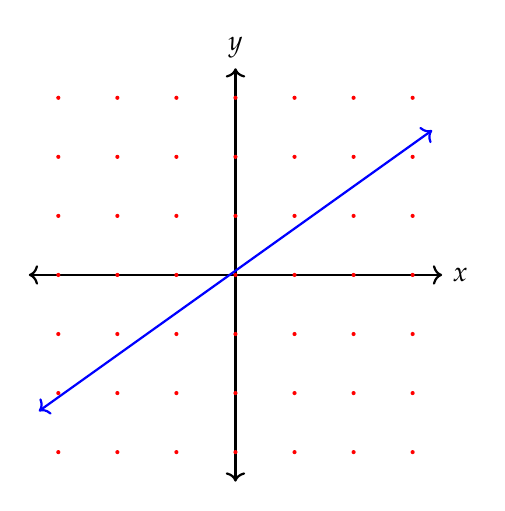
\begin{tikzpicture}[scale=0.75]
    \draw[<->,thick] (-3.5,0)--(3.5,0) node[right]{$x$};
	\draw[<->,thick] (0,-3.5)--(0,3.5) node[above]{$y$};
    \foreach \x in {-3,-2,-1,0,1,2,3}
    \foreach \y in {-3,-2,-1,0,1,2,3}
    {
    \fill[red] (\x,\y) circle (1pt);
    }
    \draw[<->,blue,thick] (-3.33,-2.307) -- (3.33,2.45);
  \end{tikzpicture}\]
Does it intersect the integer grid?\\
\\
Algebraically, let $A,B,C \in \zz$, does there exist $(x,y) \in \zz^2$ such that
\[Ax + BY = C\]

\vspace*{0.5em}

\emph{\textbf{Question}}. \textit{Can we find $(x,y) \in \zz^2$ such that $133x + 85y = 1$?}\\[0.5em]
\emph{\textbf{Discussion}}. Visually, what we're asking for is this: suppose you are standing at $0$ on the number line and you're allowed to
\begin{itemize}
\item \emph{\color{blue} hop} 133 steps left (-133) or right (+133)
\item \emph{\color{red} skip} 85 steps left (-85) or right (+85)
\end{itemize}
\vspace*{1em}
\[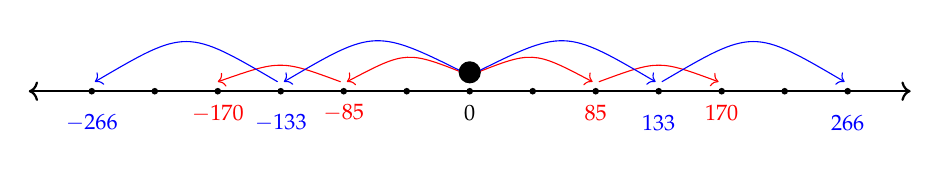
\begin{tikzpicture}[scale=0.8]
    \draw[<->,thick] (-7,0)--(7,0);
	\foreach \x in {-6,-5,-4,-3,-2,-1,0,1,2,3,4,5,6}
    {
    \fill (\x,0) circle (1.5pt);
    }
    \node[] at (0,-0.35) {\footnotesize$0$};
    \node[] at (2,-0.35) {\footnotesize\color{red}$85$};
    \node[] at (4,-0.35) {\footnotesize\color{red}$170$};
    \node[] at (-2,-0.35) {\footnotesize\color{red}$-85$};
    \node[] at (-4,-0.35) {\footnotesize\color{red}$-170$};
    \node[] at (3,-0.5) {\footnotesize\color{blue}$133$};
    \node[] at (6,-0.5) {\footnotesize\color{blue}$266$};
    \node[] at (-3,-0.5) {\footnotesize\color{blue}$-133$};
    \node[] at (-6,-0.5) {\footnotesize\color{blue}$-266$};
    \draw[red,->] (0,0.25) .. controls (1,0.65) .. (1.95,0.15);    
    \draw[red,->] (2.05,0.15) .. controls (3,0.5) .. (3.95,0.15);    
    \draw[red,->] (0,0.25) .. controls (-1,0.65) .. (-1.95,0.15);    
    \draw[red,->] (-2.05,0.15) .. controls (-3,0.5) .. (-4,0.15);    
    \draw[blue,->] (0,0.25) .. controls (1.5,1) .. (2.95,0.15);    
    \draw[blue,->] (3.05,0.15) .. controls (4.5,1) .. (5.95,0.15);    
    \draw[blue,->] (0,0.25) .. controls (-1.5,1) .. (-2.95,0.15);    
    \draw[blue,->] (-3.05,0.15) .. controls (-4.5,1) .. (-5.95,0.15);    
    \fill[] (0,0.3) circle (0.5em);
	\end{tikzpicture}\]
Then we want to know if you can hop $x$-many times and skip $y$-many times to get to $1$. For example, hopping twice to the right and skipping thrice to the left gets you
\[133\cdot (+2) + 85\cdot (-3) = 266 - 255 = 11\]
%\newpage
The answer is \textbf{yes}. The theoretical reason is the $\gcd$, \emph{greatest common divisor}, and the algorithmic reason is the \emph{(Euclidean) Division Algorithm}.

\vspace*{2em}

{\bf \large (Euclidean) Division Algorithm.}
The purpose is to check if $Ax + By = C$ has any integer solution and to find them all.
\begin{itemize}
\item Start with two positive integers $a,b$, assume $a \geq b$.
\item Divide $a$ by $b$
\[a = bq + r,\quad 0 \leq r < b,\quad q \in \zz\]
\item If $r = 0$, \textsl{halt}. If not, repeat the previous steps by replacing $(a,b)$ by $(b,r)$.
\item Continue until your remainder is $0$, this process will terminate in finite steps.
\end{itemize}
%In haiku,
%\begin{center}
%{\footnotesize
%Divisor to front,\\
%remainder to divisor,\\
%ignore the quotient.
%}
%\end{center}

\vspace*{1em}

Let's revisit the equation above, and see how the algorithm above makes it possible for us to find a required solution.
\begin{example}\label{example 1}
Employ the Division Algorithm to $(133,85)$ and find a solution to the equation $133x + 85y = 1$.
\end{example}
\begin{proof}[Answer]
Let's employ the Division Algorithm
\begin{align*}
{\color{blue} 133} &= {\color{blue} 85}\cdot (1) + {\color{red} 48}\\[0.5em]
{\color{blue} 85} &= {\color{blue} 48}\cdot (1) + {\color{red} 37}\\[0.5em]
{\color{blue} 48} &= {\color{blue} 37}\cdot (1) + {\color{red} 11}\\[0.5em]
{\color{blue} 37} &= {\color{blue} 11}\cdot (3) + {\color{red} 4}\\[0.5em]
{\color{blue} 11} &= {\color{blue} 4}\cdot (2) + {\color{red} 3}\\[0.5em]
{\color{blue} 4} &= {\color{blue} 3}\cdot (1) + {\color{red} 1}\\[0.5em]
{\color{blue} 3} &= {\color{blue} 1}\cdot (3) + {\color{red} 0}
\end{align*}
Let's take the last non-zero remainder, $1$, and work backwards in the following fashion
\begin{align*}
1 &= 4 + {\color{red} 3}\cdot (-1)\\[0.5em]
&= 4 + {\color{red} (11 - 4\cdot(2))}\cdot (-1)\\[0.5em]
&= 11\cdot (-1) + {\color{red} 4}\cdot (3)\\[0.5em]
&= 11\cdot (-1) + {\color{red} (37 - 11\cdot(3))}\cdot (3)\\[0.5em]
&= 37\cdot (3) + {\color{red} 11}\cdot (-10)\\[0.5em]
&= 37\cdot (3) + {\color{red} (48 - 37\cdot(1))}\cdot (-10)\\[0.5em]
&= 48\cdot (-10) + {\color{red} 37}\cdot (13)\\[0.5em]
&= 48\cdot (-10) + {\color{red} (85 - 48\cdot (1))}\cdot (13)\\[0.5em]
&= 85\cdot (13) + {\color{red} 48}\cdot (-23)\\[0.5em]
&= 85\cdot (13) + {\color{red} 133 - 85\cdot (1)}\cdot (-23)\\[0.5em]
&= 133\cdot ({\color{blue} -23}) + 85\cdot({\color{blue} 36})
\end{align*}
Therefore $(x,y) = (-23,36)$ is such that $133x + 85y = -3059 + 3060 = 1$.
\end{proof}

%\vspace*{1em}

\begin{example}
Does there exist a solution to the equation $91x + 49y = 1$.
\end{example}
\begin{proof}[Answer]
Let's employ the Division Algorithm as we did in the previous example
\begin{align*}
{\color{blue} 91} &= {\color{blue} 49}\cdot (1) + {\color{red} 42}\\[0.5em]
{\color{blue} 49} &= {\color{blue} 42}\cdot (1) + {\color{red} 7}\\[0.5em]
{\color{blue} 42} &= {\color{blue} 7}\cdot (6) + {\color{red} 0}
\end{align*}
Unlike the previous example where the last non-zero remainder was exactly the number on the right hand side of the given equation, we have $7$ which is not the number on the right hand side of the given equation, $1$. So, one may guess that this equation doesn't have a solution.\\
\\
One would then be correct, let's show this by way of contradiction. Suppose there did exist a pair $(x,y) \in \zz^2$ such that $91x + 49y = 1$, which gives us
\[7\cdot (13x + 7y) = 1.\]
This tells us that $7 \mid 1$ ($7$ divides $1$), which is preposterous. Therefore no solution exists.
\end{proof}

It would have been a different story if the right hand side was divisible by $7$, which happens to be $\gcd(91,49)$ and the last non-zero remainder we obtained using the division algorithm. This is not a coincidence.

\vspace*{1.5em}

\begin{remark}
The fact that the equation $133x + 85y = 1$ has a solution $(x,y) = (-23,36)$ means that $133x + 85y = c$ has a solution for any integer $c$, which is nothing but $(-23c,36c)$.
\end{remark}

\vspace*{1em}

\begin{definition}[Greatest Common Divisor]
Let $a,b$ be non-zero integers, than any positive integer $g$ is called a \emph{greatest common denominator} of $a$ and $b$, denoted $\gcd(a,b)$ or $\gcd(b,a)$, if
\begin{itemize}
\item[(D1)] $g\mid a$ and $g\mid b$, i.e. if $g$ is a common divisor; and
\item[(D2)] $d$ is any integer such that $d\mid a$ and $d\mid b$, then $d\mid g$.
\end{itemize}
\vspace{0.5em}
\emph{e.g.} $\gcd(-4,6) = 2,\ \gcd(91,49) = 7,\ \gcd(133,85) = 1$
\end{definition}

\vspace*{1em}

\begin{lemma}
The $\gcd$ for a given pair of non-zero integers is unique.
\end{lemma}
\begin{proof}
Let $a,b$ be non-zero integers and suppose $g$ and $g'$ are two $\gcd$'s of $a$ and $b$. In particular, both of them are common divisors of $a$ and $b$, therefore by (D2) we have $g\mid g'$ and $g'\mid g$. Hence $g = g'$, since $g,g'>0$ (see Problem \ref{div a}); thus, the $\gcd$ is unique.
\end{proof}

\vspace*{1em}

\begin{theorem}\label{Theorem 1.6}
Let $a,b$ be positive integers. The last non-zero remainder $R$ obtained under the Division Algorithm applied to $a$ and $b$ is equal to $\gcd(a,b)$.
\end{theorem}
\begin{proof}
To prove this theorem, we will first prove the following lemma\\
\begin{subproof}
\vspace*{-0.1in}
\begin{lemma}\label{Lemma 1.7}
Let $u,v,q,r$ be integers such that $u = vq + r$, then
\[g = \gcd(u,v) \iff g = \gcd(v,r)\]
\end{lemma}
\begin{proof}
($\Rightarrow$) Suppose $g = \gcd(u,v)$, let's prove $g = \gcd(v,r)$.
\begin{itemize}
\item[(i)] Since $g = \gcd(u,v)$, therefore $g\mid u$ and $g\mid v$. Since $u = vq + r$, hence $r = u - vq$ and thus $g\mid r$ (see Problem \ref{div a}). Therefore $g\mid v$ and $g\mid r$.
\item[(ii)] Let $d\mid v$ and $d\mid r$, then since $u = vq + r$, we have $d\mid u$. That is, $d\mid u$ and $\mid v$, and since $g = \gcd(u,v)$, by definition $g\mid d$.
\end{itemize}
By definition, we then have $g = \gcd(v,r)$. A very similar argument gives you ($\Leftarrow$).
\end{proof}
\vspace*{0.01em}
\end{subproof}
\vspace*{0.5em}
With this lemma in mind, let's assume, without loss of generality, $a\geq b$. We employ the Division Algorithm and let's assume it terminates in $n$ steps, that is our algorithm gives us the following
\begin{align*}
a &= bq_1 + r_1 & \text{(Step 1)}\\[0.25em]
b &= r_1q_2 + r_2 & \text{(Step 2)}\\[0.25em]
r_1 &= r_2q_3 + r_3 & \text{(Step 3)}\\[0.25em]
&\quad\vdots\\[0.25em]
r_{n-4} &= r_{n-3}q_{n-2} + r_{n-2} & \text{(Step $n-2$)}\\[0.25em]
r_{n-3} &= r_{n-2}q_{n-1} + R & \text{(Step $n-1$)}\\[0.25em]
r_{n-2} &= Rq_n + 0 & \text{(Step $n$)}
\end{align*}
Our Lemma \ref{Lemma 1.7} tells us that
\[\gcd(a,b) = \gcd(b,r_1) = \gcd(r_1,r_2) = \cdots = \gcd(r_{n-3},r_{n-2}) = \gcd(r_{n-2},R)\]
Note that in (Step $n$) we have obtained $R\mid r_{n-2}$ and therefore $\gcd(r_{n-2},R) = R$ (see Problem \ref{gcd a}). Hence $R = \gcd(a,b)$, as needed to be shown.
\end{proof}

\vspace*{1em}

\begin{example}[in-class]
Consider the pair $(39,14)$, using the Division Algorithm determine $\gcd(39,14)$ and find a solution to $39x + 14y = \gcd(39,14)$.
\end{example}

%\vspace*{1em}

We distil the above theorem and the Division Algorithm into the following major theorem.
\begin{theorem}[B\'ezout's Identity]
Given non-zero integers $a,b$, there exist integers $x,y$ such that
\[ax + by = \gcd(a,b)\]
\end{theorem}
\begin{proof}
Consider $|a|,|b|>0$, then by Theorem \ref{Theorem 1.6} and working the Division Algorithm backwards as in Example \ref{example 1} we find integers $x,y$ such that 
\[|a|x + |b|y = \gcd(a,b)\]
\begin{itemize}
\item \emph{Case I.} If $a,b>0$, then $(x,y)$ is the pair we want.
\item \emph{Case II.} If $a>0,b<0$, then $(x,-y)$ is the pair we want.
\item \emph{Case III.} If $a<0,b>0$, then $(-x,y)$ is the pair we want.
\item \emph{Case IV.} If $a,b<0$, then $(-x,-y)$ is the pair we want.
\end{itemize}
\vspace*{-1.2\baselineskip}
\end{proof}

\vspace*{0.2in}

\subsection{Problems}
\vspace{0.1in}

\begin{problem}[Divisibility]\label{div a}
Consider integers $x,y$, we say that $x$ divides $y$, denoted $x\mid y$, if there exists an integer $u$ such that $y = xu$.\\[0.5em]
Let $a,b,c$ be integers, then show that
\begin{itemize}
\item[(i)] if $a\mid b$ and $b \neq 0$, then $|a| \leq |b|$.
\item[(ii)] if $a\mid b$, then $a\mid bc$.
\item[(iii)] if $a\mid b$ and $b\mid c$, then $a\mid c$.
\item[(iv)] if $c\mid a$ and $c\mid b$, then $c\mid (am + bn)$ for any integer $m$ and $n$.
\item[(v)] if $a\mid b$ and $b\mid a$, then $a = \pm b$.
\item[(vi)] if $c \neq 0$, then $a\mid b$ if and only if $ac\mid bc$.
\end{itemize}
\end{problem}

\vspace*{0.1in}

\begin{problem}\label{gcd a}
Let $a,b$ be non-zero integers. Prove that
\begin{itemize}
\item[(i)] $\gcd(a,0) = |a|$; $\gcd(a,1) = 1$.
\item[(ii)] if $b\mid a$, then $\gcd(a,b) = b$.
\item[(iii)] $\gcd(a,a+1) = 1$; 
\item[(iv)] $\gcd(a,b) = \gcd(|a|,|b|)$.
\item[(v)] $\gcd(ka,kb) = |k|\gcd(a,b)$, for all $k \in \zz$.
\item[(vi)] if $\gcd(a,k) = \gcd(b,k) = 1$, then $\gcd(ab,k) = 1$, for all $k \in \nn$.
\item[(vii)] if $\gcd(a,b) = 1$, then $\gcd(a^m,b^n) = 1$, for all $m,n \in \nn$.
\end{itemize}
\end{problem}

\vspace*{0.1in}

\begin{problem}\label{gcd b}
Let $a,b,c$ be integers, and let $g\coloneqq \gcd(a,\gcd(b,c))$. 
\begin{itemize}
\item[(i)] Prove that $g$ satisfies the following properties
\begin{itemize}
\item[(P1)] $g\mid a$, $g\mid b$ and $g\mid c$, i.e., $g$ is a common divisor of $a,b$ and $c$
\item[(P2)] If $d$ is a common divisor of $a,b$ and $c$, then $d\mid g$.
\end{itemize}
\item[(ii)] Show that $g = \gcd(b,\gcd(a,c)) = \gcd(c,\gcd(a,b))$
\end{itemize}
For this reason, we will write $\gcd(a, b, c) \coloneqq \gcd(a, \gcd(b, c))$, and call it \emph{the} greatest common divisor of $a, b$ and $c$.
\end{problem}

\vspace*{0.1in}

\begin{problem}\label{gcd c}
Using Problem \ref{gcd b} define $\gcd(a_1,\ldots,a_n)$ for integers $a_1,\ldots,a_n$, where $n \geq 4$.
\end{problem}
\newpage

\section{Lecture 2 (9/28)}
\vspace*{1em}

We are concerned with finding solutions to the equation
\begin{align*}\label{lde}
Ax + By = C \tag{$\bigstar$}
\end{align*}
where $A,B,C \in \zz$ and $A,B \neq 0$.

\vspace*{1em}

\begin{theorem}[Existence of a Solution]
\refp{lde} has a solution if and only if $g \coloneqq \gcd(A,B) \mid C$.
\end{theorem}
\begin{proof}
($\Rightarrow$) Suppose there exists a solution $(x,y) \in \zz^2$ such that 
\[Ax + By = C.\]
Since $g = \gcd(A,B)$, then $g\mid A$ and $g\mid B$, therefore $g\mid (Ax+ By) = C$.\\
\\
($\Leftarrow$) Let $g\mid C$, then $C = gD$ for some integer $D$. By B\'ezout's Identity, there exist integers $x_0,y_0$ such that 
\[Ax_0 + By_0  = g,\quad \text{then } C = gD = A(x_0D) + B(y_0D).\]
Therefore $(x,y) = (x_0D,y_0D)$ solves \refp{lde}.
\end{proof}

\vspace*{1em}

\begin{example}\label{example 2.1}
Find $x,y \in \zz$ that solves $27x + 105y = 81$.
\end{example}
\begin{proof}[Answer]
We first employ the Division Algorithm to compute $\gcd(27,105)$
\begin{align*}
105 &= 27\cdot(3) + 24\\[0.25em]
27 &= 24\cdot (1) + 3\\[0.25em]
24 &= 3\cdot(8) + 0
\end{align*}
By Theorem \ref{Theorem 1.6}, $\gcd(27,105) = 3$, and since $3\mid 81$, therefore the given equation has a solution. We now work the above calculation backwards
\begin{align*}
3 &= 27 - 24\cdot(1)\\[0.25em]
&= 27 - (105 - 27\cdot(3)) = 27\cdot (4) + 105\cdot(-1)
\end{align*}
Hence
\[81 = 27\cdot 3 = 27\cdot (27\cdot 4) + 105\cdot(27\cdot(-1)) = 27\cdot (108) + 105\cdot (-27)\]
Thus $(x,y) = (108,-27)$ solves the given equation.
\end{proof}

\vspace*{1em}

\begin{definition}[Least Common Multiple]
Let $a,b$ be non-zero integers, than any positive integer $\ell$ is called a \emph{least common multiple} of $a$ and $b$, denoted $\lcm(a,b)$ or $\lcm(b,a)$, if
\begin{itemize}
\item[(M1)] $a\mid \ell$ and $b\mid \ell$, i.e. if $\ell$ is a common multiple; and
\item[(M2)] $m$ is any integer such that $a\mid m$ and $b\mid m$, then $\ell\mid m$.
\end{itemize}
\vspace{0.5em}
\emph{e.g.} $\lcm(-4,6) = 12,\ \lcm(91,49) = 637$
\end{definition}

\vspace{2em}

{\bf\large Goal.} We want to compute the set $\setp{(x,y)\in \zz^2}{Ax + By = C}$ provided $\gcd(A,B) \mid C$, because otherwise this set is empty.\\
\\
Our previous discussions tell us that we know how to find $(x_0,y_0) \in \zz^2$ such that
\begin{align*}\label{geq1}
Ax_0 + By_0 = C \tag{1}
\end{align*}
Suppose $(x_1,y_1)$ is another solution, that is
\begin{align*}\label{geq2}
Ax_1 + By_1 = C \tag{2}
\end{align*}
Then \refp{geq2} $-$ \refp{geq1} gives us 
\begin{align*}\label{geql}
Ax' + By' = 0 \tag{L}
\end{align*}
where $x' = x_1 - x_0$ and $y' = y_1 - y_0$.

\vspace*{2em}

\begin{proposition}\label{proposition 2.4}
Let $A,B \in \zz$, then
\begin{itemize}
\item[(i)] for any $n\in \zz$, let
\[x' = n\cdot \frac{\lcm(A,B)}{A} \quad\text{and}\quad y' = -n\cdot \frac{\lcm(A,B)}{B}.\]
Then $Ax' + By' = 0$, that is $(x',y') \in \zz^2$ solves \refp{geql}
\item[(ii)] All integer solutions to \refp{geql} are of the form given in (i).
\end{itemize}
\begin{proof}
For the given $(x',y')$ we have
\begin{align*}
Ax' + By' &= A\left(n\cdot \frac{\lcm(A,B)}{A}\right) + B\left(-n\cdot \frac{\lcm(A,B)}{B}\right) = 0,
\end{align*}
thus proving (i).\\
\\
Suppose $x",y" \in \zz$ were solutions to \refp{geql}, that is $Ax" + By" = 0$. Let 
\[m \coloneqq Ax" = B(-y"),\]
then $A\mid m$ and $B \mid m$. By definition, $\lcm(A,B)\mid m$, therefore $m = n'\cdot\lcm(A,B)$ for some integer $n'$. Giving us
\begin{align*}
Ax" &= m = n'\cdot \lcm(A,B) & B(-y") &= m = n'\cdot \lcm(A,B)
\end{align*}
Therefore
\begin{align*}
x"&= n'\cdot\frac{\lcm(A,B)}{A} & y"&= -n'\cdot\frac{\lcm(A,B)}{B};
\end{align*}
hence (ii) is proved.
\end{proof}
\end{proposition}

%\vspace*{1em}

\begin{theorem}[Algorithm to Solve \refp{lde}]\label{ldea}\hfill
\begin{itemize}
\item Compute $\gcd(A,B)$ using the Division Algorithm.
\item If $\gcd(A,B)\nmid C$, there exists no solution.
\item If $\gcd(A,B) \mid C$, then let $g = \gcd(A,B)$ and $C = gD$
\begin{itemize}
\item[(i)] use the Division Algorithm on $A,B$, and work backwards to find $(x_0',y_0') \in \zz^2$ such that $Ax_0' + By_0' = g$.
\item[(ii)] then $(x_0,y_0) = (x_0'D,y_0'D)$ is a particular solution to $Ax + By = C$
\item[(iii)] the general solution will then be 
\[\begin{cases}x = x_0 + n\cdot\dfrac{\lcm(A,B)}{A}\\[1.5em] y = y_0 - n\cdot\dfrac{\lcm(A,B)}{B}\end{cases}\]
for any $n \in \zz$. For a given integer $n$, let the corresponding solution be $(x_n,y_n)$.
\end{itemize}
\end{itemize}
\end{theorem}
\begin{proof}
The only thing we need to prove is (iii). Let $(x',y')$ be any other solution to \refp{lde}, i.e. $Ax' + By' = C$. Then
\[Ax" + By" = 0,\]
where $x" = x' - x_0$ and $y" = y' - y_0$. Therefore
\[x" = n\cdot\frac{\lcm(A,B)}{A}\quad\text{and}\quad y" = -n\cdot\frac{\lcm(A,B)}{B}\]
by Proposition \ref{proposition 2.4}. Hence
\[x' = x_0 + n\cdot\dfrac{\lcm(A,B)}{A} \quad\text{and}\quad y' = y_0 - n\cdot\dfrac{\lcm(A,B)}{B}\]
and thus we have proved (iii).
\end{proof}

\vspace*{1em}

\begin{example}
Find all solutions to the equation $27x + 105y = 81$.
\end{example}
\begin{proof}[Answer]
We have found a particular solution $(x_0,y_0) = (108,-27)$ to the given equation in Example \ref{example 2.1}. Further, we can calculate the $\lcm$ as follows (we will prove this later)
\[\lcm(27,105) = \frac{27\cdot 105}{\gcd(27,105)} = \frac{27\cdot 105}{3} = 945.\]
Therefore, the general solution is
\begin{align*}
x &= 108 + n\cdot \frac{945}{27} = 108 + 35n\\[0.5em]
y &= -27 - n\cdot \frac{945}{105} = -27 - 9n
\end{align*}
That is, the set of all solutions to the given equation is $\setp{(108 + 35n,-27 - 9n)}{n \in \zz}$
\end{proof}

\newpage
%\vspace*{1em}

\begin{example}[in-class]
Find all solutions to the equation $117x + 42y = 33$.
\end{example}

\vspace*{2em}

\begin{center}
{\Large Prime Factorisation}
\end{center}

\begin{definition}
Let $n > 0$ be an integer.
\begin{itemize}
\item $n$ is prime (or a prime number) if $n> 1$ and $1$ and itself are its only divisors.
\item $n$ is composite if $n>1$ and is not a prime; equivalently, $n = ab$ for some integers $1<a,b<n$.
\item $n = 1$ is called a unit.
\end{itemize}
\end{definition}

\vspace*{1em}

\begin{lemma}\label{primediv}
Let $a,b,c \in \zz$. If $a\mid bc$ and $\gcd(a,b) = 1$ (that is, $a$ and $b$ are coprime), then $a\mid c$. 
\end{lemma}
\begin{proof}
Since $\gcd(a,b) = 1$, by B\'ezout's Identity, there exist integers $x,y$ such that 
\[1 = ax + by,\qquad \text{therefore}\quad c = acx + bcy\]
Clearly $a\mid ac$ and, by assumption, $a\mid bc$, hence $a\mid c$.
\end{proof}

\vspace*{1em}

\begin{corollary}[useful property of primes]
Let $p$ be a prime number and $b,c \in \zz$. If $p\mid bc$, then $p\mid b$ or $p\mid c$. 
\end{corollary}
\begin{proof}
Suppose $p\mid b$, then we have nothing to prove. So assume that $p\nmid b$, and consider $g \coloneqq \gcd(p,b)$. So, $g\mid p$ and therefore $g = 1$ or $g = p$. If $g = p$, then we have $g\mid b$, a contradiction; hence $g = 1$. Thus, by Lemma \ref{primediv} we get $p\mid c$.
\end{proof}

\vspace*{1em}

\begin{theorem}[Fundamental Theorem of Arithmetic AKA Unique Prime Factorisation]\label{fundarith}
\hfill\\[0.2em]
Let $n$ be any positive integer.
\begin{itemize}
\item[1.] (existence) $n$ admits a prime factorisation, i.e. there exist integers $e_p \geq 0$ for each prime $p$ such that 
\begin{itemize}
\item[$\bullet$] $e_p = 0$, for all $p > n$
\item[$\bullet$] $n = 2^{e_2}\cdot 3^{e_3}\cdots p^{e_p}\cdots$
\end{itemize}
\item[2.] (uniqueness) Suppose $n$ admits another prime factorisation, say $n = 2^{f_2}\cdot 3^{f_3}\cdots p^{f_p}\cdots$. Then, for every prime $p$, we have $e_p = f_p$.
\end{itemize}
In particular, $n$ has a prime factor.
\end{theorem}
\begin{proof}[Proof (skipped in class)] We prove existence of prime factorization by inducting on $n$. For $n = 1$ and $n = 2$, we note that 
\begin{align*}
1 = 2^{e_2}\,3^{e_3}\cdots p^{e_p}\cdots, &\quad \text{where $e_p = 0$ for every prime $p$}\\[0.5em]
2 = 2^{e_2}\,3^{e_3}\cdots p^{e_p}\cdots, &\quad \text{where $e_2 = 1$ and $e_p = 0$ for every prime $p>2$}
\end{align*}
Hence the existence statement holds true for $n = 1$ and $n = 2$. Assume that the existence statement is true for every positive integer $< n$. So, consider $n$ itself; if $n$ is prime itself, then
\begin{align*}
n = 2^{e_2}\,3^{e_3}\cdots n^{e_n} \cdots p^{e_p}\cdots, &\quad \text{where $e_n = 1$ and $e_p = 0$ for every prime $p \neq n$};
\end{align*}
in particular $e_p = 0$ for any prime $p> n$, so the existence statement holds. Now, suppose that if $n$ was composite instead, then necessarily $n = ab$ for integers $1 < a,b < n$. By our assumption, both $a$ and $b$ possess prime factorizations, say
\[a = 2^{i_2}\,3^{i_3}\cdots q^{i_q}\cdots \qquad \text{and} \qquad b = 2^{j_2}\,3^{j_3}\cdots r^{j_p}\cdots,\]
where the exponents are positive integers, and $i_q = j_r = 0$ for every prime $q > a$ and $r > b$, in particular $i_p = j_p = 0$ for every prime $p > n$ since $n>a,b$. Therefore,
\[n = ab = 2^{i_2 + j_2}\,3^{i_3 + j_3}\cdots p^{i_p + j_p}\cdots,\]
where the exponents are again, necessarily, positive integers and we have $i_p + j_p = 0$ for every prime $p > n$. Hence, the existence statement is true for $n$.  Therefore, by the principal of mathematical induction, the existence statement is true for every integer $n$.\\
\\
Let's now prove the uniqueness statement, suppose an integer $n > 0$ possesses the following prime factorizations
\[n = 2^{e_2}\,3^{e_3}\cdots p^{e_p}\cdots = 2^{f_2}\,3^{f_3}\cdots p^{f_p}\cdots,\]
where the exponents satisfy the properties in the existence statement. For the sake contradiction, suppose that there exists a prime $q$ such that $e_q \neq f_q$; let's assume, without loss of generality, that $e_q < f_q$. Define $d_q = f_q - e_q > 0$, and consider 
\[\frac{n}{e_q} = 2^{e_2}\,3^{e_3}\cdots q^{0}\cdots = 2^{f_2}\,3^{f_3}\cdots q^{d_q}\cdots.\]
Then note that $q$ divides the latter expression since $d_q > 0$, so it should divide the former expression. But since the exponent of $q$ is $0$ in the former expression, $q$ necessarily does not divide it. Hence we have arrived at a contradiction, thus $e_p = f_p$ for every prime $p$ and the uniqueness statement follows.
\end{proof}

\vspace*{1em}

%\begin{remark}
%In particular, this theorem tells us that every positive integer has a prime factor.
%\end{remark}
%\vspace*{1em}

\begin{proposition}\label{primeprod}
Let $a,b$ be positive integers with the following prime factorisation
\[a = 2^{e_2}\cdot 3^{e_3}\cdots p^{e_p}\cdots,\quad b = 2^{f_2}\cdot 3^{f_3}\cdots p^{f_p}\cdots\]
Then
\begin{itemize}
\item[(i)] $ab = 2^{e_2 + f_2}\cdot 3^{e_3 + f_3}\cdots p^{e_p + f_p}\cdots$.
\item[(ii)] $a\mid b$ if and only if $e_p \leq f_p$, for every prime $p$.
\end{itemize}
\end{proposition}
\begin{proof} 
(i) is a direct result of power rules. Let's prove (ii).\\[0.5em]
($\Rightarrow$) Suppose $a\mid b$, then $b = ac$ for some positive integer $c$. Let $c = 2^{g_2}\cdot 3^{g_3}\cdots p^{g_p}\cdots$, then
\[b = ac = 2^{e_2+g_2}\cdot 3^{e_3+g_3}\cdots p^{e_p+g_p}\cdots\]
By uniqueness of prime factorisation we have $f_p = e_p + g_p \geq g_p$ for every prime $p$.\\[0.5em]
($\Leftarrow$) Suppose $e_p \leq f_p$, define $g_p \coloneqq f_p - e_p \geq 0$ for every prime $p$. Let $c\coloneqq 2^{g_2}\cdot 3^{g_3}\cdots p^{g_p}\cdots$, then by definition $b = ac$, and therefore $a\mid b$.
\end{proof}

%\vspace*{1em}

\vspace*{0.2in}

\subsection{Problems}
\vspace{0.1in}

\begin{problem}\label{problem 2.1}
Let $a,b,c \in \zz$. If $a\mid bc$ and $\gcd(a,b) = d$, then prove that $a\mid dc$.
\end{problem}

\vspace*{0.1in}

\begin{problem}\label{problem 2.2}
Let $a,b,c \in \zz$. Prove that $\gcd(a,b) = 1$ if and only if $\gcd(a^2,b^2) = 1$.
\end{problem}

\vspace*{0.1in}

\begin{problem}\label{problem 2.3}
Let $a,b \in \zz$. Then prove that if $g = \gcd(a,b)$, then $\gcd\left(\dfrac{a}{g},\dfrac{b}{g}\right) = 1$.
\end{problem}

\vspace*{0.1in}

\begin{problem}\label{problem 2.4}\hfill
\begin{itemize}
\item[(i)] Using the Division Algorithm, find a particular solution $(x,y)$ to the equation $150x + 111y = 15$.
\item[(ii)] Proceed to find all the integer solutions to the equation  $150x + 111y = 15$.
\item[(iii)] Find all the integer solutions $(x, y)$ to the equation $-187x + 68y = 288$. (If none exists, prove it.)
\end{itemize}
\end{problem}

\vspace*{0.1in}

\begin{problem}\label{problem 2.5}
Look at Problem \ref{gcd b}, write and prove the statements analogous for the $\lcm$. 
\end{problem}

\vspace*{0.1in}

\begin{problem}\label{problem 2.6}\hfill
\begin{itemize}
\item[(i)] Prove that there exists no integer solution $(x, y, z)$ to the equation
\[18x - 27y + 39z = 4.\]
\item[(ii)] Find \emph{an} integer solution $(x, y, z)$ to the equation \[18x - 27y + 39z = 6.\]
\item[(iii)] (challenge) Find \emph{all} integer solutions $(x, y, z)$ to the equation $18x - 27y + 39z = 6$.\\[0.5em]
Your answer should give explicit formulae for $x, y, z$ in terms of three free independent integer parameters $m$ and $n$ (not unlike the case of two variables where we have one independent integer parameter).
\end{itemize}
\end{problem}

\vspace*{0.1in}

\begin{problem}\label{problem 2.7}
Let $a,b$ and $n$ be positive integers, and $a^n \mid b^n$, prove that $a\mid b$.
\end{problem}

\vspace*{0.1in}

\begin{problem}\label{problem 2.8}
Recall that $n! = 1\cdot 2\cdots (n-1)\cdot n$. Prove that if $n\geq 1$, then no number in the following list of $n-1$ numbers
\[n! + 2,\, n! + 3,\,\ldots,\, n! + n\]
is a prime.\\[0.5em]
This problem illustrates that there's no bound on the length of gaps between primes.
\end{problem}

%\vspace*{0.1in}

%\begin{problem}\label{problem 2.9}
%This problem relates the prime factorisation of factorials.
%\begin{itemize}
%\item[(a)] Find the prime factorisation of $20!$.
%\item[(b)] How many zeros would you find at the end of $100!$, if you expand it out in base ten?
%\item[(c)] Let $e_p$ be the exponent of $p$ in the prime factorisation of $n!$. Prove that
%\[e_p \leq \frac{n}{p-1}\]
%{\footnotesize Hint: use the geometric series
%\[p^{-1} + p^{-2} + p^{-3} + \cdots = p^{-1}(1 + p^{-1} + p^{-2} + \cdots) = \frac{1}{p-1}\]
%}
%\end{itemize}
%\end{problem}
\newpage

\section{Lecture 3 (9/30)}
\vspace*{1em}

\begin{lemma}\label{gcdform}
With the notation as in Proposition \ref{primeprod}, we have
\begin{align*}
\gcd(a,b) &= 2^{\min(e_2,f_2)}\cdot 3^{\min(e_3,f_3)}\cdots p^{\min(e_p,f_p)}\cdots\\[0.5em]
\lcm(a,b) &= 2^{\max(e_2,f_2)}\cdot 3^{\max(e_3,f_3)}\cdots p^{\max(e_p,f_p)}\cdots
\end{align*}
In particular, $ab = \gcd(a,b)\lcm(a,b)$.
\end{lemma}
\begin{proof}
Suppose we have proven that the $\gcd$ and $\lcm$ have the given prime factorisation, then since $e_p + f_p = \min(e_p,f_p) + \max(e_p,f_p)$, therefore $ab = \gcd(a,b)\lcm(a,b)$.\\
\\
Write $g \coloneqq \gcd(a,b) = 2^{h_2}\cdot 3^{h_3}\cdots p^{h_p}$. Since $g\mid a$ and $g\mid b$, therefore $h_p \leq e_p$ and $h_p \leq f_p$ and hence $h_p \leq \min(e_p,f_p)$.\\[0.5em]
Let $d = 2^{\min(e_2,f_2)}\cdot 3^{\min(e_3,f_3)}\cdots p^{\min(e_p,f_p)}\cdots$, since $\min(e_p,f_p) \leq e_p$ and $\min(e_p,f_p) \leq f_p$, therefore $d\mid a$ and $d\mid b$. Hence $d\mid g$, by definition of $\gcd$, thus $\min(e_p,f_p) \leq h_p$.\\[0.5em]
Therefore $h_p = \min(e_p,f_p)$, and hence $\gcd(a,b) = 2^{\min(e_2,f_2)}\cdot 3^{\min(e_3,f_3)}\cdots p^{\min(e_p,f_p)}\cdots$. A similar argument gives us the result for $\lcm$.
\end{proof}

\vspace*{1em}

\begin{example}
Consider
\begin{align*}
a &= 180 = 2^2\cdot 3^2\cdot 5 = 2^2\cdot 3^2\cdot 5^1\cdot 7^0\\[0.5em]
b &= 126 = 2\cdot 3^2\cdot 7 = 2^1\cdot 3^2\cdot 5^0\cdot 7^1
\end{align*}
Find their $\gcd$ and $\lcm$. How many positive divisors of $b$ can there be?
\end{example}
\begin{proof}[Answer]
By Corollary \ref{gcdform}, we have
\begin{align*}
\gcd(a,b) &= 2^1\cdot 3^2\cdot 5^0\cdot 7^0 = 18\\[0.5em]
\lcm(a,b) &= 2^2\cdot 3^2\cdot 5^1\cdot 7^1 = 1260
\end{align*}
Now, any positive divisor of $b$ is necessarily of the form $d = 2^{e_2}\cdot 3^{e_3}\cdot 7^{e_7}$. By Proposition \ref{primeprod}, 
\[0 \leq e_2 \leq 1,\quad 0\leq e_3 \leq 2,\quad 0 \leq e_7 \leq 1,\]
therefore the number of positive divisor of $b$ is $2\cdot 3\cdot 2 = 12$, since $e_2$ has two choices, $e_3$ has three and $e_7$ has two as well.
\end{proof}

\vspace*{1em}

\begin{example}[in-class]
Consider
\begin{align*}
a &= 3^2\cdot 5^4\cdot 11^1\cdot 17^3\\[0.5em]
b &= 2^3\cdot 3^2\cdot 5^3\cdot 7^2
\end{align*}
Compute the prime factorisation of their $\gcd$ and $\lcm$. How many positive divisors does $a$ have?
\end{example}

%\vspace*{1em}

Another important consequence of unique prime factorisation of positive integers
\vspace*{0.5em}
\begin{theorem}\label{bijection}
Let $a$ and $b$ be coprime positive integers
\begin{itemize}
\item[(i)] If $u$ and $v$ are positive divisors of $a$ and $b$ respectively, then $uv \mid ab$. 
\item[(ii)] Conversely, for any positive divisor $w$ of $ab$, there exist positive integers $u$ and $v$ such that $u\mid a$ and $v\mid b$, and $w = uv$.
\end{itemize}
In short, there's a bijection
\[\Phi:\mathscr{D}(a) \times \mathscr{D}(b) \to \mathscr{D}(ab),\quad \Phi(u,v) = uv\]
where (non-standard notation) $\mathscr{D}(n) \coloneqq \setp{d \in \zz_+}{d\mid n}$, i.e. the set of positive divisors of $n$.
\end{theorem}
\begin{proof}
(i) follows from Problem \ref{div a}. Let's prove (ii): consider a positive divisor $w$ of $ab$, where the prime factorisation of $a$ and $b$ is written as
\[a = p_1^{e_1} p_2^{e_2}\cdots p_r^{e_r},\quad b = q_1^{f_1}q_2^{f_2}\cdots q_s^{f_s}\]
Since $\gcd(a,b) = 1$, necessarily $p_i \neq q_j$ for all $1\leq i \leq r,\ 1\leq j \leq s$. Therefore
\[ab = p_1^{e_1} p_2^{e_2}\cdots p_r^{e_r}q_1^{f_1}q_2^{f_2}\cdots q_s^{f_s},\]
and hence 
\[w = p_1^{h_1} p_2^{h_2}\cdots p_r^{h_r}q_1^{k_1}q_2^{k_2}\cdots q_s^{k_s},\]
where $0 \leq h_i \leq e_i$ and $0 \leq k_j \leq f_j$, by Proposition \ref{primeprod}. Letting $u = p_1^{h_1} p_2^{h_2}\cdots p_r^{h_r}$ and $v = q_1^{k_1}q_2^{k_2}\cdots q_s^{k_s}$, gives us $w = uv$ and, again by Proposition \ref{primeprod}, $u\mid a$ and $v\mid b$.\\
\\
This proves surjectivity of $\Phi$, injectivity follows from uniqueness of prime factorisation.
\end{proof}

\vspace*{1em}

\begin{definition}
For any positive integer $n$, 
\[\sigma_0(n) \coloneqq \card\,\mathscr{D}(n),\]
that is, the number of positive divisors of $n$.
\vspace*{0.5em}\\
\emph{e.g.}\quad $\sigma_0(6) = \card\set{1,2,3,6} = 4$
\end{definition}

\vspace*{0.5em}

\begin{remark}
$\sigma_0(n) = 1$ if and only if $n = 1$. If $n > 1$, then $\sigma_0(n) \geq 2$ since $n$ always has $1$ and $n$ as divisors. In fact, $\sigma_0(n) = 2$ if and only if $n$ is prime.
\end{remark}

\vspace*{1em}

\begin{corollary}\label{multsigma0}
For coprime positive integers $a,b$, we have $\sigma_0(ab) = \sigma_0(a)\sigma_0(b)$.
\end{corollary}
\begin{proof}
Recall the bijection $\Phi$ from Theorem \ref{bijection}, therefore the cardinalities of the domain and codomain of $\Phi$ are equal. The cardinality of the domain being $\sigma_0(a)\sigma_0(b)$ and that of the domain being $\sigma_0(ab)$. Hence $\sigma_0(ab) = \sigma_0(a)\sigma_0(b)$.
\end{proof}

\vspace*{0.5em}

\begin{corollary}\label{sigma0formula}
For a positive integer $n$ with prime factorisation given as $n = p_1^{e_1} p_2^{e_2}\cdots p_r^{e_r}$, we have
\[\sigma_0(n) = (e_1+1)(e_2+1)\cdots(e_r+1)\]
\end{corollary}
\begin{proof}
Let $p$ be a prime, then note that $\mathscr{D}(p^e) = \setp{p^f}{0\leq f \leq e}$ for any integer $e\geq 0$, and therefore $\sigma_0(p^e) = e + 1$. Now, consider $n$ as in the statement, then applying Corollary \ref{multsigma0} iteratively we have
\begin{align*}
\sigma_0(n) &= \sigma_0(p_1^{e_1} p_2^{e_2}\cdots p_r^{e_r})\\[0.5em]
&= \sigma_0(p_1^{e_1})\, \sigma_0(p_2^{e_2})\cdots \sigma_0(p_r^{e_r}).
\end{align*}
Then by our observations above, we get $\sigma_0(n) = (e_1+1)(e_2+1)\cdots(e_r+1)$.
\end{proof}

\vspace*{1em}

{\bf\large Appreciating unique prime factorisation.} First, we make a small extension to our definitions: any non-zero integer can be uniquely written as
\[n = \pm 2^{e_2}\cdot 3^{e_3}\cdots p^{e_p}\cdots,\quad \text{such that $e_p \geq 0$ and $e_p = 0$ for all $p > |n|$}\]
$\pm 1$ are called units.

\vspace*{1em}

\begin{definition}
$\mathscr{O} = \zz[\sqrt{-5}] \coloneqq \setp{a+b\sqrt{-5}}{a,b \in \zz} \subseteq \cc$
\[\begin{tikzpicture}
    \draw[<->,thick] (-3.5,0)--(3.5,0) node[right]{$\Re$};
	\draw[<->,thick] (0,-3)--(0,3) node[above]{$\Im$};
    \foreach \x in {-3,-2,-1,0,1,2,3}
    \foreach \y in {-2.5,-1.25,0,1.25,2.5}
    {
    \fill[red] (\x,\y) circle (1pt);
    }
    \node[] at (0.4,1.5) {{\footnotesize $\sqrt{-5}$}};
  \end{tikzpicture}\]
  \\
{\bf\large Fact.} $\mathscr{O}$ is closed under addition, subtraction and multiplication, and also contains $0$ and $1$. That is, $\mathscr{O}$ is a (commutative) ring.
\end{definition}
\begin{proof}[Sketch of Fact]
Let $\alpha = a + b\sqrt{-5}$ and $\beta = c + d\sqrt{-5}$ be elements of $\mathscr{O}$, then
\begin{align*}
\alpha + \beta &= (a + c) + (b + d)\sqrt{-5} \in \mathscr{O}\\[0.5em]
-\beta &= (-c) + (-d)\sqrt{-5} \in \mathscr{O}\\[0.5em]
\alpha\beta &= (ac - 5bd) + (ad + bc)\sqrt{-5} \in \mathscr{O}
\end{align*}
$0 = 0 + 0\sqrt{-5}$ and $1 = 1 + 0\sqrt{-5}$.
\end{proof}

%\vspace*{3em}

We'll mimic the definition of prime numbers in $\zz$ and introduce the notion of prime elements in the set $\mathscr{O}$.

\vspace*{1em}

\begin{definition}
A non-zero element $\alpha$ is called a \emph{prime element} of $\mathscr{O}$ if
\begin{itemize}
\item[(P1)] $\alpha \neq \pm 1$
\item[(P2)] for any $\beta,\gamma \in \mathscr{O}$ such that $\alpha = \beta\gamma$, then necessarily $\beta = \pm 1$ or $\gamma = \pm 1$
\end{itemize}
\end{definition}

%\vspace*{1em}

$\mathscr{O}$ does not admit a notion of \emph{unique} prime factorisation, that is, elements in $\mathscr{O}$ can have two distinct prime factorisations. We illustrate this fact with an example, the content of which is Problem \ref{ufd}; note
\begin{align*}
6 &= 2\cdot 3 = (1 + \sqrt{-5})(1- \sqrt{-5})
\end{align*}
and we also know that there exists no $\gamma \in \mathscr{O}$ such that $2\gamma = 1 \pm \sqrt{-5}$.

\vspace*{0.5in}

\subsection{Problems}
\vspace{0.1in}

\begin{problem}\label{problem 3.1}
Look at Problem 14, book.
Let $a,b$ be positive integers. Prove that $\gcd(a^k,b^k) = \gcd(a,b)^k$ and $\lcm(a^k,b^k) = \lcm(a,b)^k$ for any integer $k \geq 0$.
\end{problem}

\vspace*{0.1in}

\begin{problem}\label{problem 3.2}
Let $a,b$ and $k$ be positive integers, then prove that $\gcd(ka,kb) = k\cdot \gcd(a,b)$ and $\lcm(ka,kb) = k\cdot \lcm(a,b)$.
\end{problem}

\vspace*{0.1in}

\begin{problem}\label{problem 3.3}
Write the prime factorisation of $N = 13!$ and compute $\sigma_0(N)$.
\end{problem}

\vspace*{0.1in}

\begin{problem}\label{problem 3.4}
As in class, consider the collection of complex numbers of the form:
\[\mathscr{O} = \setp{a + bi\sqrt{5}}{a, b \in \zz}.\]
\begin{itemize}
\item[(a)] Consider the integer-valued function $\operatorname{N}$ defined on $\mathscr{O}$:
\[\operatorname{N}(a + bi\sqrt{5}) = a^2 + 5b^2.\]
Prove that
\[\operatorname{N}(\alpha\beta) = \operatorname{N}(\alpha)N(\beta)\]
for any two elements $\alpha$ and $\beta$ in $\mathscr{O}$.
\item[(b)] Say that an element $\alpha$ in $\mathscr{O}$ is a \textbf{prime element} (prime elements are analogues of prime numbers) if
\begin{itemize}
\item[(i)] $\alpha \neq 0, \pm 1$; and
\item[(ii)] whenever we have $\alpha = \gamma \delta$ with $\gamma, \delta$ in $\mathscr{O}$, we necessarily have $\gamma = \pm 1$ or $\delta = \pm 1$.
\end{itemize}
Prove that the following $4$ elements are prime elements: $2$, $3$, $1 + \sqrt{-5}$ and $1 - \sqrt{-5}$.\\[0.5em]
{\footnotesize Hint: proceed by way of contradiction, then use part (a).} 
\item[(c)] Show that there exists no element $\gamma$ in $\mathscr{O}$ such that $2\gamma = 1+\sqrt{-5}$ or $2\gamma = 1-\sqrt{-5}$.
\end{itemize}
Conclusion: Prime factorisation in $\mathscr{O}$ is not unique: $2 \cdot 3 = 6 = (1 + \sqrt{-5})(1 - \sqrt{-5})$.
\end{problem}

\vspace*{0.1in}

\begin{problem}\label{problem 3.5}
Let $T = \set{1,4,7,10,13,16,19,\ldots}$. An element of $T$ is called \emph{irreducible} if it is not $1$ and its only factors \emph{within $T$} are $1$ and itself.
\begin{itemize}
\item[(a)] Suppose $a,b \in T$ and $c$ is a positive integer. Prove that if $a = bc$, then $c\in T$.
\item[(b)] Demonstrate that every element of $T$ can be factored as a product of irreducible elements of $T$. 
\item[(c)] Find three examples of elements of $T$ with \emph{nonunique} factorisation into irreducibles.
\end{itemize}
\end{problem}

\vspace*{0.1in}

\begin{problem}\label{problem 3.6}
Prove that if $n$ is a positive integer, and $\sigma_0(n)$ is prime then $n$ is a power of a prime number.
\end{problem}

\vspace*{0.1in}

\begin{problem}\label{problem 3.7}
What is the smallest positive integer with precisely $60$ positive divisors?
\end{problem}
\newpage

\section{Lecture 4 (10/5)}
\vspace{1em}

{\bf\large Distribution of prime numbers I. \emph{Larger scale}}
\vspace*{0.5em}
\begin{theorem}[Euclid]
There are infinitely many primes.
\end{theorem}
\begin{proof}
Towards a contradiction, assume there are finitely many primes
\[p_1 = 2,\, p_2 = 3,\ldots,\,p_N\]
Consider $M = p_1p_2\cdots p_N + 1$, since every positive integer has a prime factor, $p_i \mid M$ for some $1\leq i \leq N$.\\[0.5em]
But also note that $p_i \mid p_1p_2\cdots p_N$, and therefore $p_i$ divides $M - p_1p_2\cdots p_N = 1$, giving us a contradiction. Hence, there are infinitely many primes.
\end{proof}

\vspace*{2.5em}

More quantitatively,
\begin{definition}
For any real number $x>0$,
\[\pi(x) \coloneqq \text{number of primes} \leq x\]
$\pi$ is called the \emph{prime counting function}.
\vspace*{1em}\\
\emph{e.g.}\quad $\pi(1.5) = 0$,\ $\pi(23) = \card\set{2,3,5,7,11,13,17,19,23} = 9$.
\end{definition}

\vspace*{2em}

So, Euclid's theorem says that as $\pi(x) \to \infty$ as $x \to \infty$. Computing $\pi(x)$ is hard, one can do it for $x \sim 10^{13}$ but not for, say, $x \sim 10^{10^{10}}$.\\[1em]
\begin{itemize}[leftmargin=4.8em]
\item[\emph{\textbf{Question.}}] Do we have an asymptotic formula for $\pi(x)$?\\[0.5em]
That is, can we find a simpler function $f$ such that 
\[\lim_{x\to \infty}\frac{\pi(x)}{f(x)} = 1\]
If so, can we bound the "error" $|\pi(x) - f(x)|$ in terms of $x$?
\end{itemize}

\vspace*{1em}

\begin{theorem}[Prime Number Theorem, (1896) Hadamard, de la Vall\'ee Poussin]
\[\lim_{x \to \infty}\frac{\pi(x)}{\mathrm{Li}(x)} = 1,\]
where $\displaystyle \mathrm{Li}(x) = \int_2^x \dfrac{dt}{\log t} \sim \dfrac{x}{\log x}$
\end{theorem}

%\vspace*{1em}

\begin{conjecture}[a consequence of the Riemann Hypothesis]
For all $x \geq 2657$,
\[|\pi(x) - \mathrm{li}(x)| < \frac{1}{8\pi}\,\sqrt{x}\log x,\]
where $\displaystyle \mathrm{li}(x) = \int_0^x \dfrac{dt}{\log t} = \mathrm{Li}(x) - \ln 2$.
\end{conjecture}

\vspace*{3em}

{\bf\large Distribution of prime numbers I. \emph{Smaller scale}}
\vspace*{0.5em}
\begin{align*}
\underbracket{2,\ 3}_1,\ 5,\ 7,\ 11,\ 13,\ &\ldots,\ 263,\ 269,\ 271,\ 277,\ \ldots,\\[0.5em]
& 877,\ 881,\ 883,\ 887,\ 907,\ \ldots
\end{align*}
Since all primes, bigger than $2$, are odd, so the gap between them is always even; except between $2$ and $3$.

\vspace*{2em}
 
\begin{definition}
\emph{Twin primes} are a pair of primes $(p,q)$ such that $|p-q| = 2$.
\end{definition}

\vspace*{1em}

\begin{conjecture}
There are infinitely many twin primes.
\end{conjecture}

\vspace*{1em}

\begin{theorem}
There are infinitely many pairs $(p,q)$ of primes such that 
\begin{align*}
\textnormal{($\sim 2013$, Y. Zhang)}\quad & |q-p| < 7\cdot 10^7\\[0.5em]
\textnormal{($\sim 2014$, Polymath8)}\quad & |q-p| < 246
\end{align*}
\end{theorem}

\vspace*{2em}

{\bf\large Sum of Divisor functions.}
\vspace*{0.5em}
\begin{definition}
A function $f:\zz_+ \to \cc$ is called \emph{multiplicative} if $f(ab) = f(a)f(b)$, for coprime positive integers $a,b$.
\vspace{0.5em}\\
\begin{proof}[e.g.]\renewcommand{\qedsymbol}{}
\begin{itemize}
\item[(1)] Fix $k \in \rr$, define $f_k(n) = n^k$. Then $f_k(ab) = (ab)^k = a^kb^k = f_k(a)f_k(b)$.
\end{itemize}
\begin{itemize}[leftmargin=4.4em]
\item[(2)] Recall $\sigma_0:\zz_+ \to \cc$, where $\sigma_0(n) = \text{number of positive divisors of $n$}$. Corollary \ref{multsigma0} tells us that $\sigma_0$ is multiplicative.\\[0.5em]
Note that the coprime assumption is essential; consider, for instance, $a = 2$ and $b = 4$, then $\sigma_0(2\cdot 4) = \sigma_0(8) = 4$. But $\sigma_0(2) = 2$ and $\sigma_0(4) = 3$, therefore $\sigma_0(2)\sigma_0(4) = 6 \neq 4 = \sigma_0(2\cdot 4)$.
\end{itemize}
\begin{itemize}[leftmargin=6em]
\item[\emph{non-example.}] Consider the function $f: \zz_+ \to \cc$ given as $f(n) = 2n+1$. Then note for $a = 2$ and $b = 3$, we have
\[f(2\cdot 3) = f(6) = 11\]
\[f(2) = 3;\quad f(3) = 5\]
Of course, $f(2\cdot 3) = 11 \neq 15 = f(2)f(3)$.
\end{itemize}
\end{proof} 
\end{definition}

%\vspace*{0.2em}

\begin{definition}
Let $k \in \rr$, define 
\[\sigma_k:\zz_+ \to \cc\]
as $\sigma_k(n) =$ sum of $k$-power of positive divisors of $n$, that is
\[\sigma_k(n) = \sum_{d \in \mathscr{D}(n)}d^k\]
\emph{Special Case.} When $k = 0$, then $\sigma_0(n) = \sum_{\,d\in \mathscr{D}(n)}d^0 = \card\,\mathscr{D}(n) = \text{number of positive divisors of $n$}$.\\[1em]
\emph{e.g.}\quad $k = 2,\ \sigma_2(6) = 1^2 + 2^2 + 3^2 + 6^2 = 50$.
\end{definition}

\vspace*{1.5em}

\begin{theorem}
For any $k \in \rr,\ \sigma_k$ is multiplicative.
\end{theorem}
\begin{proof}
Let $a,b$ be positive integers such that $\gcd(a,b) = 1$, then
\begin{align*}
\sigma_k(ab) = \sum_{w\in \mathscr{D}(ab)}w^k &= \sum_{(u,v)\in \mathscr{D}(a) \times \mathscr{D}(b)}(uv)^k ,\quad \text{by Theorem \ref{bijection}}\\[0.5em]
&= \sum_{u \in \mathscr{D}(a)}\sum_{v \in \mathscr{D}(a)}u^kv^k\\[0.5em]
&= \sum_{u \in \mathscr{D}(a)}u^k\left(\sum_{v \in \mathscr{D}(a)} v^k\right)\\[1em]
&= \sum_{u \in \mathscr{D}(a)}u^k\sigma_k(b)\\[0.5em]
&= \sigma_k(b)\left(\sum_{u \in \mathscr{D}(a)}u^k\right) = \sigma_k(b)\sigma_k(a)
\end{align*}
Therefore $\sigma_k(ab) = \sigma_k(a)\sigma_k(b)$, whenever $\gcd(a,b) = 1$.
\end{proof}

\vspace*{1em}

We're now ready to introduce a strategy to compute $\sigma_k(n)$ for any given $k$ and $n$, but first we review a proposition that we need.

\vspace*{0.5em}

\begin{proposition}\label{geomsum}
Let $x\neq 1$ be a real number and $e$ be a non-negative integer. Then 
\[1 + x + x^2 + \cdots + x^e = \frac{x^{e+1}-1}{x-1}\]
\end{proposition}
\begin{proof}
Let $S = 1 + x + x^2 + \cdots + x^{e-1} + x^e$, then
\begin{align*}
xS &= x + x^2 + \cdots + x^e + x^{e+1}\\[0.5em]
&= x + x^2 + \cdots + x^e + x^{e+1} + 1 - 1\\[0.5em]
&= (1 + x + x^2 + \cdots + x^e) + x^{e+1} - 1\\[0.5em]
&= S + x^{e+1} - 1
\end{align*}
Therefore $(x-1)S = xS- S = x^{e+1} - 1$. Since $x\neq 1$, hence $\displaystyle S = \frac{x^{e+1}-1}{x-1}$.
\end{proof}

\vspace*{1em}

\begin{corollary}\label{sigprimeform}
If $p$ is a prime, $e \geq 0$ an integer and $k \neq 0$, then
\[\sigma_k(p^e) = \frac{(p^{e+1})^k - 1}{p^k - 1}\]
\end{corollary}
\begin{proof}
Note that for any $d \in \mathscr{D}(p^e)$, we necessarily have $d = p^f,\ 0 \leq f \leq e$ (in particular, $\sigma_0(p^e) = e + 1$). Therefore
\begin{align*}
\sigma_k(p^e) &= (p^0)^k + (p^1)^k + (p^2)^k + \cdots + (p^{e-1})^k + (p^e)^k\\[0.5em]
&= 1 + p^k + (p^k)^2 + \cdots + (p^k)^e\\[0.5em]
&= \frac{(p^k)^{e+1} - 1}{p^k - 1},\quad \text{taking $x = p^e$ in Proposition \ref{geomsum}}
\end{align*}
since $k \neq 0$.
\end{proof}

\vspace*{1em}

\begin{example}
Compute $\sigma_3(12)$.
\end{example}
\begin{proof}[Answer]
First note that $12 = 2^2\cdot 3$. Since $\gcd(2^2,3) = 1$, therefore 
\begin{align*}
\sigma_3(12) &= \sigma_3(2^2)\sigma_3(3)\\[0.5em]
&= \frac{(2^{2+1})^3 - 1}{2^3 - 1}\cdot\frac{(3^{1+1})^3 - 1}{3^3 - 1} = 73\cdot 28.
\end{align*}
Hence $\sigma_3(12) = 2044$.
\end{proof}

\vspace*{1em}

So our general strategy to compute $\sigma_k(n)$, when $k>0$, is as follows:
\begin{itemize}
\item Consider the prime factorisation of $n$, say $n = p_1^{e_1}\cdots p_r^{e_r}$
\item Since $\gcd(p_i,p_j) = 1$, therefore $\gcd(p_i^{e_i},p_j^{e_j}) = 1$ for $i \neq j$ (see Problem \ref{gcd a}).
\item Hence $\sigma_k(n) = \sigma_k(p_1^{e_1})\cdots\sigma_k(p_r^{e_r})$.
\item Apply Corollary \ref{sigprimeform} to $\sigma_k(p_i^{e_i})$.
\end{itemize}

%\vspace*{1em}

One reason why we care about $\sigma_k$

\vspace*{0.5em}

\begin{definition}
Let $n$ be a positive integer
\begin{itemize}
\item[(1)] Say $n$ is \emph{perfect} if the sum of proper divisors of $n$, that is divisors strictly less than $n$, equals $n$. Equivalently, if $\sigma_1(n) = 2n$.
\item[(2)] Say $n$ is \emph{deficient} if $\sigma_1(n) < 2n$.
\item[(3)] Say $n$ is \emph{abundant} if $\sigma_1(n) > 2n$.
\end{itemize}
\vspace*{0.5em}
\begin{proof}[e.g.]\renewcommand{\qedsymbol}{}
\begin{itemize}
\item[(1)] Let $n = p$ be a prime, then $\sigma_1(p) = 1 + p < 2p$. Therefore primes are deficient.
\end{itemize}
\begin{itemize}[leftmargin=4.4em]
\item[(2)] Let $n = 6$, then $\sigma_1(6) = 1 + 2 + 3 + 6 = 6 + 6$. Therefore $6$ is perfect.
\item[(3)] Let $n = 12$, then $\sigma_1(12) = 1 + 2 + 3 + 4 + 6 + 12 > 24$. Therefore $24$ is abundant.
\end{itemize}
\end{proof}
\end{definition}

\vspace*{-1em}

\emph{Known perfect numbers:} $6,\,28,\,496,\,8128,\,33550336,\ldots$ (about fifty).

\vspace*{1em}

\begin{proof}[Open Questions]\renewcommand{\qedsymbol}{}
\hfill
\begin{itemize}
\item are there infinitely many perfect numbers?
\item are there any \emph{odd} perfect numbers?
\end{itemize}
\end{proof}

%\vspace*{1em}

\begin{example}[in-class]
\hfill
\begin{itemize}
\item[(i)] Express $\sigma_4(27)$ as $\dfrac{3^a - 1}{3^b - 1}$ for some positive integers $a,b$.
\item[(ii)] Suppose we're given a multiplicative function $f$, and we've been told 
\[f(2) = 4,\quad f(3) = 11,\quad f(4) = 3,\quad f(6) = 33,\quad f(8) = 5\]
Do we know enough to compute $f(24)$? If yes, compute it. If not, why not?
\end{itemize}
\end{example}

\vspace*{2em}

\emph{\textbf{Question}}. \textit{For which $n \in \zz_+$, is $2^n - 1$ prime?}

\vspace*{1em}

\begin{proposition}\label{mersprime}
If a positive integer $n$ is such that $2^n - 1$ is prime, then $n$ is prime.
\end{proposition}
\begin{proof}
Suppose, for sake of contradiction, $n$ is not prime. Then $n = ab$, for some $1<a,b<n$, which gives us
\begin{align*}
2^n - 1 &= 2^{ab}-1\\[0.5em]
&= (2^a)^b - 1^b\\[0.5em]
&= (2^a - 1)((2^a)^{b-1}+(2^a)^{b-2}+\cdots+2^a+1)
\end{align*}
These are non-unit proper divisors of $2^{ab} - 1$, since $1<a,b<n$. Therefore this number is composite, giving us a contradiction. Hence $n$ is prime.
\end{proof}

%\vspace*{1em}

\emph{\textbf{The converse is not true}}, that is, if $n$ is prime then $2^n - 1$ is not necessarily prime.
\vspace*{0.5em}\\
\emph{e.g.}\quad $2^{11} - 1 = 2047 = 23\cdot 89$.

\vspace*{0.5in}

\subsection{Problems}
\vspace{0.1in}

\begin{problem}\label{problem 4.1}
For this problem, you may want to review one-variable Calculus.
\begin{itemize}
\item[(a)] Recall the definition 
\[\mathrm{Li}(x) = \int_2^x \frac{dt}{\log t}\quad \text{for } x > 2\]
What is $\dfrac{d}{dx}\mathrm{Li}(x)$?
\item[(b)] Prove that \[\lim_{x\to \infty}\frac{\mathrm{Li}(x)}{x/\log x} = 1.\]
\end{itemize}
\end{problem}

\vspace*{0.1in}

\begin{problem}\label{problem 4.2}
Compute $\sigma_1(N)$ for the three numbers $N = 28,\ N = 111$, and $N = 240$. Classify $N$ as abundant, deficient or perfect.
\end{problem}

%\newpage
\vspace*{0.1in}

\begin{problem}[Mersenne, 1644]\label{problem 4.3}
Describe all circumstances under which $\sigma_1(n)$ is odd.
\end{problem}

\vspace*{0.1in}

\begin{problem}\label{problem 4.4}
Find a short formula for $\sigma_0(p) + \sigma_1(p) + \cdots + \sigma_k(p)$ whenever $p$ is a prime number.
\end{problem}

\vspace*{0.1in}

\begin{problem}\label{problem 4.5}
Prove that for every positive integer $n$, we have
\[\sigma_k(n) = \sigma_{-k}(n)n^k.\]
Conclude that $n$ is perfect if and only if $\sigma_{-1}(n) = 2$.
\end{problem}

\vspace*{0.1in}

\begin{problem}\label{problem 4.6}
Prove that if $n$ is a perfect square, then $n$ is not a perfect number.
\end{problem}

\vspace*{0.1in}

\begin{problem}\label{problem 4.7}
We say that a positive integer $n$ is \emph{square-free} if $n$ is not divisible by $p^2$ for any prime number $p$. Necessarily, $n$ is then a distinct product of primes. (E.g. $15$ and $37$ are square-free, but $24$ and $49$ are not.)\\[0.5em]
Consider the function $\mu$ (named after A.F. M{\"o}bius, popularly known for his strip) defined on positive integers $n$ as follows:
\[\mu(n) = \begin{cases}1 & \text{if $n = 1$}\\[0.5em] 0 & \text{if $n$ is not square-free}\\[0.5em] (-1)^t & \text{if $n$ is square-free and has exactly $t$ prime divisors.} \end{cases}\]
\begin{itemize}
\item[(a)] Compute $\mu(n)$ for $n = 1,\ldots,15$.
\item[(b)] Prove that $\mu$ is multiplicative, i.e., we have $\mu(ab) = \mu(a)\mu(b)$ whenever $a$ and $b$ are positive coprime integers.\\
{\footnotesize Hint: proceed by cases, taking cue from the definition of $\mu$.}
\item[(c)] Let $n > 1$ be any integer greater than $1$. Prove that
\[\sum_{d\in \mathscr{D}(n)} \mu(d) = 0.\]
In other words, the sum of $\mu(d)$, as $d$ ranges over all the positive divisors of $n$, is equal to $0$. 
\end{itemize}
\end{problem}

\vspace*{0.1in}

\begin{problem}\label{problem 4.8}
Let $f(n)$ and $g(n)$ be two complex-valued multiplicative functions of positive integers $n$. Define $h(n)$ by the formula:
\[h(n) = \sum_{d\in \mathscr{D}(n)}f(d)g\left(\frac{n}{d}\right).\]
\begin{itemize}
\item[(a)] Consider the case where $g(n) = \mu(n)$ defined in Problem \ref{problem 4.7} above and $f(n) = n$. Compute the values of $h(n)$ for $n = 1,\ldots,12$.
\item[(b)] Prove, in the general case of multiplicative functions $f$ and $g$, that $h$ is a multiplicative function.
\end{itemize}
(The new function $h$ is called the \textit{convolution} of $f$ and $g$, and is denoted by $f \star g$. The idea originates from Fourier analysis.)
\end{problem}
\newpage

\section{Lecture 5 (10/7)}
\vspace*{1em}

We relate perfect numbers with certain kinds of prime numbers.

\vspace*{1em}

\begin{definition}
A \emph{Mersenne prime} is a prime number $M_p$ of the form $2^p - 1$ for some prime $p$.
\end{definition}
\emph{e.g.}\quad $M_3 = 2^3 - 1 = 7$ is a Mersenne prime, but $11$ is not since $11+1$ is not a power of $2$.

\vspace*{1em}

\begin{theorem}[Euclid]\label{mersiseven}
Let $M_p$ be a Mersenne prime, then $N_p = 2^{p-1}M_p = 2^{p-1}(2^p - 1)$ is an even perfect number.
\vspace*{0.5em}\\
e.g.\quad $M_2 = 3,\ N_2 = 6;\ M_3 = 7,\ N_3 = 28;\ M_5 = 31,\ N_5 = 496$.
\end{theorem}
\begin{proof}
Recall that $\sigma_1(n) = \sum_{\,d\in \mathscr{D}(n)}d$, and that $n$ is a perfect number if and only if $\sigma_1(n) = 2n$. Furthermore, since $M_p$ is an odd prime, necessarily $\gcd(2^{p-1},M_p) = 1$. Consider
\begin{align*}
\sigma_1(N_p) &= \sigma_1(2^{p-1}M_p)\\[0.5em]
&= \sigma_1(2^{p-1})\cdot\sigma_1(M_p),\quad \text{since $\gcd(2^{p-1},M_p) = 1$ and $\sigma_1$ is multiplicative}\\[0.5em]
&= \frac{2^{p-1+1} - 1}{2 - 1}\cdot(1 + M_p)\\[0.5em]
&= 2^p(2^p - 1)\\[0.5em]
&= 2\cdot 2^{p-1}M_p\\[0.5em]
&= 2N_p
\end{align*}
Therefore $N_p$ is an even perfect number.
\end{proof}

\vspace*{1em}

\begin{theorem}[Euler, 1849]
Suppose $N$ is an even perfect number, then there exists a prime number $p$ such that $N = N_p$, as in Theorem \ref{mersiseven}.
\end{theorem}
\begin{proof}
Let $N$ have the following prime factorisation 
\[N = 2^{e_2}\cdot 3^{e_3}\cdots p^{e_p}\cdots,\]
where $e_p \geq 0$ (and $e_p = 0$ for all $p>N$). Let $p \coloneqq e_2 + 1$ and $q \coloneqq N/2^{e_2} = 3^{e_3}\cdots p^{e_p}\cdots$. In particular, $N = 2^{p-1}q$.\\[0.5em]
Note that $\gcd(2^{p-1},q) = 1$ since $2\nmid q$. Since $N$ is perfect, we have
\begin{align*}
2^pq = 2N = \sigma_1(N) &= \sigma_1(2^{p-1}q)\\[0.5em]
&= \sigma_1(2^{p-1})\cdot\sigma_1(q),\quad \text{since $\sigma_1$ is multiplicative}\\[0.5em]
&= (2^p - 1)\cdot\sigma_1(q)
\end{align*}
Therefore, 
\begin{align*}
\sigma_1(q) &= q\cdot\left(\frac{2^p}{2^p - 1}\right) = q\cdot\left(\frac{1}{2^p - 1} + 1\right) = \frac{q}{2^p - 1} + q
\end{align*}
Since $\sigma_1(q)$ and $q$ are integers, so is $\sigma_1(q) - q = \dfrac{q}{2^p - 1}$.  That is,
\[d \coloneqq \dfrac{q}{2^p - 1} \in \zz_+\]
Hence, $q = d\cdot(2^p - 1)$ and thus $d\mid q$. Since $N$ is even $p - 1 = e_2 \geq 1$, so $2^p - 1 > 1$ and therefore $d \neq q$, i.e., $d$ is a proper divisor of $q$. Hence, $\sigma_1(q) = q + d$.
\begin{itemize}
\item \emph{Case I: $q = 1$.} Then $d = \sigma_1(1) - 1 = 0$, giving us a contradiction since $d$ is positive.
\item \emph{Case II: $q$ is composite.} Then $q = ab$, for some positive integers $a,b$ such that $1<a,b<n$. We have the following two possibilities
\begin{itemize}
\item[$\diamond$] \emph{$a$ or $b$ equal $d$.} Suppose $a = d$, without loss of generality, then $d = \sigma_1(q) - q \geq d + b > d$. We have arrived at a contradiction.
\item[$\diamond$] \emph{neither $a$ nor $b$ equal $d$.} Then $d = \sigma_1(q) - q \geq d + a + b > d$. We have arrived at a contradiction again.
\end{itemize}
\end{itemize}
Hence $q$ is prime, and thus necessarily $d = 1$, since it's a proper divisor of $q$. That is, $q = 2^p - 1$ is a prime, and so $p$ is prime by Proposition \ref{mersprime}. Thus, $q = M_p$ is a Mersenne prime and $N = N_p$.
\end{proof}

%\newpage
\vspace*{2em}

\begin{center}
{\Large Rational Numbers}
\end{center}

\begin{definition}
A \emph{rational number} is a number of the form $\dfrac{a}{b}$, where $a,b$ are integers and $b \neq 0$.\\[0.1em]
A \emph{fraction} is an expression of the form $\dfrac{a}{b}$, where $a,b$ are integers and $b \neq 0$.
\end{definition}
\emph{e.g.}\quad $\dfrac{2}{3}$ and $\dfrac{4}{6}$ are distinct fractions but equal as rational numbers.

\vspace*{1em}

\begin{definition}
Say a fraction $\dfrac{a}{b}$ is \emph{reduced} if $\gcd(a,b) = 1$ and $b> 0$.
\end{definition}
\emph{e.g.}\quad $\dfrac{2}{3}$ is reduced but $\dfrac{4}{6}$ isn't.\quad $\dfrac{2}{-3}$ isn't reduced but $\dfrac{-2}{3} = -\dfrac{2}{3}$ is.

\vspace*{1em}

\begin{theorem}\label{reducedfraction}
Let $\dfrac{a}{b}$ be a fraction, then there exists a unique fraction $\dfrac{c}{d}$ such that $\dfrac{a}{b} = \dfrac{c}{d}$ as rational numbers.
\end{theorem}
\begin{proof}[e.g.]\renewcommand{\qedsymbol}{}
$-1.56 = \dfrac{156}{-100} = \dfrac{39}{-25} = -\dfrac{39}{25}$
\end{proof}

\vspace*{1em}

\begin{proposition}
If $x$ is a nonzero rational number, then there exist unique integer $e_2,e_3,\ldots,e_p,\ldots$ indexed by prime numbers, such that
\begin{itemize}
\item[(1)] all but finitely many of $e_p$'s are $0$.
\item[(2)] $x = \pm 2^{e_2}\cdot 3^{e_3}\cdots p^{e_p}\cdots$.
\end{itemize}
\end{proposition}
\begin{proof}[Proof (sketch)]
Write $x = \dfrac{a}{b}$ in reduced form, and let
\begin{align*}
a &= \pm 2^{f_2}\cdot 3^{f_3}\cdots p^{f_p}\cdots\\[0.5em]
b &= 2^{g_2}\cdot 3^{g_3}\cdots p^{g_p}\cdots
\end{align*}
where $f_p,g_p \geq 0$. Then taking $e_p \coloneqq f_p - g_p$ gives us $x = \pm 2^{e_2}\cdot 3^{e_3}\cdots p^{e_p}\cdots$.
\end{proof}
\vspace*{0.5em}
\emph{e.g.}\quad $-1.56 = -\dfrac{39}{25} = -\dfrac{3\cdot 13}{5^2} = -2^0\cdot 3^1\cdot 5^{-2}\cdot 7^0\cdot 11^0\cdot 13^1$

\vspace*{1em}

\begin{definition}
A complex number is \emph{irrational} if it's not rational
\end{definition}
\begin{proof}[e.g.]\renewcommand{\qedsymbol}{}
$\sqrt{2}$ is irrational. 
\end{proof}

\vspace*{1em}

More generally,

\begin{proposition}
Let $a/b$ be a reduced fraction and let $n\geq 2$ be an integer. Then $\alpha = \sqrt[n]{a/b}$ if and only if $a$ and $b$ are $n^{\text{th}}$ powers.
\end{proposition}
\begin{proof}
($\Rightarrow$) Suppose $\alpha$ is rational, so write $\alpha = c/d$ in reduced form, that is $\gcd(c,d) = 1$ and $d>0$. Then
\[\frac{a}{b} = \alpha^n = \frac{c^n}{d^n}\]
Since $\gcd(c,d) = 1$, therefore $\gcd(c^n,d^n) = \gcd(c,d)^n = 1$ by Problem \ref{problem 3.1} and, of course, $d^n>0$ since $d>0$. Hence $c^n/d^n$ is in reduced form, and thus by the uniqueness statement in Theorem \ref{reducedfraction} we get $a = c^n$ and $b = d^n$.\\
\\
($\Leftarrow$) If $a$ and $b$ are $n^{\text{th}}$ powers, i.e., $a = c^n$ and $b = d^n$ for some integers $c,d$. Then $\alpha = \sqrt[n]{a/b} = c/d$, and hence $\alpha$ is rational.
\end{proof}
%\vspace*{0.5em}
\begin{proof}[e.g.]\renewcommand{\qedsymbol}{}
\begin{itemize}
\item[(1)] $\sqrt{18}$ is irrational. Two ways to conclude this, $18 = 2\cdot 3^2$. For $18$ to be a square, the exponents in its prime factorisation necessarily need to be even. Alternatively, assume $18 = n^2$, then $16<18 = n^2<25$, and hence $4 < n < 5$ which isn't possible. So $18$ is not a square, and so $\sqrt{18}$ is irrational.
\end{itemize}
\begin{itemize}[leftmargin=4.4em]
\item[(2)] $\sqrt[4]{3/5}$ is irrational; since, as primes, $3$ and $5$ cannot be fourth powers.
\end{itemize}
\end{proof}

%\vspace*{1em}

\begin{definition}
Say a complex number $\alpha$ is \emph{algebraic} if it's a root of a nonzero polynomial $P(T) = c_dT^d + \cdots + c_1T + c_0$, where $c_i \in \zz$ with at least one of them being nonzero. That is, $P(\alpha) = c_d\alpha^d + \cdots + c_1\alpha + c_0 = 0$.\\[0.5em]
Otherwise, that is if $\alpha$ is not algebraic, then say $\alpha$ is \emph{transcendental}.
\end{definition}
\begin{proof}[e.g.]\renewcommand{\qedsymbol}{}
\begin{itemize}
\item[(0)] Rational numbers are algebraic: let $\alpha = a/b$, then $\alpha$ is a root of $P(T) = bT-a$.
\end{itemize}
\begin{itemize}[leftmargin=4.4em]
\item[(1)] $\sqrt{2}$ is irrational \emph{but} algebraic, it's a root of $P(T) = T^2 - 2$.
\item[(2)] More generally, consider $\alpha = \sqrt[n]{a/b}$ where $a/b$ is any rational number, then $\alpha$ is algebraic. Since $\alpha$ is a zero of $P(T) = bT^n - a$. For example, $-1$ is a root of $P(T) = T^2 + 1$.
\item[(3)] $2\sqrt{2} + \sqrt{3}$ is algebra. Let's show this.
\end{itemize}
\vspace*{0.3em}
{\bf\large Fact.} If $\alpha$ and $\beta$ are algebraic, then 
\[\alpha + \beta,\quad \alpha - \beta,\quad \alpha\beta,\quad \alpha/\beta \text{ (provided $\beta \neq 0$)}\]
are all also algebraic.
\vspace*{0.3em}
\begin{itemize}[leftmargin=4.4em]
\item[(3)] \emph{continued}. We want to find a polynomial $P(T)$ such that $P(2\sqrt{2} + \sqrt{3}) = 0$. Consider
\begin{align*}
\alpha &= 2\sqrt{2} + \sqrt{3}\\[0.5em]
\alpha - \sqrt{3} &=  2\sqrt{2}\\[0.5em]
(\alpha - \sqrt{3})^2 &=  (2\sqrt{2})^2\\[0.5em]
\alpha^2 - 2\sqrt{3}\alpha + 3 &= 8\\[0.5em]
\alpha^2 - 5 &= 2\sqrt{3}\alpha\\[0.5em]
(\alpha^2 - 5)^2 &= (2\sqrt{3}\alpha)^2\\[0.5em]
\alpha^4 - 10\alpha^2 + 25 &= 12\alpha^2
\end{align*}
Therefore $\alpha^4 - 22\alpha^2 + 25 = 0$. Hence, by construction, $P(T) = T^4 - 22T^2 + 25$ is such that $P(\alpha) = 0$. Thus $\alpha$ is algebraic.
\end{itemize}
\vspace*{-\baselineskip}
\end{proof}

\vspace*{0.5in}

\subsection{Problems}
\vspace{0.1in}

\begin{problem}\label{Problem 5.1}
Prove Theorem \ref{reducedfraction}.
\end{problem}

\vspace*{0.1in}

\begin{problem}\label{Problem 5.2}\hfill
\begin{itemize}
\item[(a)] Let $a$ and $b$ be rational numbers such that $a + b\sqrt{2} = 0$. Prove that we necessarily have $a = 0$ and $b = 0$. {\footnotesize (In terms of Linear Algebra: $1$ and $\sqrt{2}$ are $\qq$-linearly independent.)}
\item[(b)] Prove that there exist no rational numbers $a$ and $b$ such that
\[a + b\sqrt{2} = \sqrt{3}.\]
{\footnotesize Hint: start with squaring the purported equation.}
\item[(c)] Prove that there exist no rational numbers $a,\ b$ and $c$ such that
\[a + b\sqrt{2} + c\sqrt{3} = \sqrt{6}.\]
{\footnotesize Hint: what is the inverse of $\sqrt{2} - c$?} 
\item[(d)] Prove that there exist no rational numbers $a,\ b,\ c$ such that
\[a + b\sqrt{2} + c\sqrt{3} = \sqrt{5}.\]
\item[(e)] (challenge) Prove that there exist no rational numbers $a,\ b,\ c$ and $d$ such that
\[a + b\sqrt{2} + c\sqrt{3} + d\sqrt{6} = \sqrt{5}.\]
\end{itemize}
\end{problem}

\vspace*{0.1in}

\begin{problem}\label{Problem 5.3}
The aim of this problem is to prove that $\qq^{\text{alg}}$, the set of all algebraic numbers, is countable. A set $S$ is said to be countable, if there exists an injective function $f:S \to \nn$.
\begin{itemize}
\item[(a)] Prove that a countable union of countable sets is countable.
\item[(b)] Assuming $\qq$ is countable, prove $\qq^n$ is countable, for any natural number $n$.
\item[(c)] Let $P_n$ be the set of all polynomials of degree $n$ with rational coefficients, prove $P_n$ is countable.
\item[(d)] Consider
\[R_n \coloneqq \bigcup_{p(x) \in P_n}\setp{\alpha \in \cc}{p(\alpha) = 0}\]
Prove that $R_n$ is countable. Why is $R_n$ infinite?
\item[(f)] Conclude that the set of algebraic numbers is countable.
\end{itemize}
\end{problem}
\newpage

\section{Lecture 6 (10/12)}
\vspace*{1em}

The following result can be used to conclude if an algebraic number is irrational.
\vspace*{0.5em}
\begin{theorem}[Rational Root Theorem]
Let $a/b$ be a rational number in reduced form such that it's a root of a polynomial
\[P(T) = c_dT^d + c_{d-1}T^{d-1} + \cdots + c_1T + c_0\]
where $c_i \in \zz$. Then $a\mid c_0$ and $b\mid c_d$.
\end{theorem}
\begin{proof}
By assumption
\[P\left(\frac{a}{b}\right) = c_d\left(\frac{a}{b}\right)^d + c_{d-1}\left(\frac{a}{b}\right)^{d-1} + \cdots + c_1\left(\frac{a}{b}\right) + c_0 = 0\]
Then
\[c_da^d + c_{d-1}a^{d-1}b + \cdots c_1ab^{d-1} + c_0b^d = 0\]
Therefore,
\begin{align*}
c_da^d &= -b(c_{d-1}a^{d-1}+\cdots + c_1ab^{d-2})\text{; and}\\[0.5em]
c_0b^d &= -a(c_da^{d-1} +\cdots + c_1b^{d-1})
\end{align*}
Therefore $b\mid c_da^d$ and $a\mid c_0b^d$. Since $\gcd(a,b) = 1$, hence $\gcd(a,b^d) = \gcd(a^d,b) = 1$. Thus $b\mid c_d$ and $a\mid c_0$, by Lemme \ref{primediv}.
\end{proof}

\emph{e.g.}\quad For $\alpha = 2\sqrt{2} + \sqrt{3}$, we found $P(T) = T^4 - 22T^2 + 25$ is such that $P(\alpha) = 0$. Suppose $\alpha = a/b$ is rational, then $a\mid 25$ and $b\mid 1$. Therefore $a/b \in \set{\pm 1, \pm 5, \pm 25}$ but none of them equal $2\sqrt{2} + \sqrt{3}$.

\vspace*{1em}

\begin{example}[in-class]
$\sqrt{3} + \sqrt{5}$ is algebraic and irrational.
\end{example}

\vspace*{1em}

{\bf Examples of transcendental number.} Note that $\cc$ is uncountable but the set of all algebraic numbers is countable. Therefore there are uncountably many transcendental numbers.

\vspace*{1em}

\begin{theorem}[Lindemann \& Weierstrass, 1800's]
$\pi$ and $e$ are transcendental.\\
\\
\textnormal{(But we don't yet know if $e + \pi$ is transcendental, for example.)}
\end{theorem}

\vspace*{1em}

\begin{corollary}[ancient]
We cannot square the circle. That is, using only a straight ruler and compass we cannot construct a square whose area is equal to $\pi$.
\end{corollary}

\vspace*{1.5em}

{\bf Other suspects.} Let $k \geq 1$ be an integer, then
\[\zeta_k = 1 + \frac{1}{2^k} + \frac{1}{3^k} + \frac{1}{4^k} + \cdots\]
converges when $k>1$.
\begin{proof}[{\bf Facts}]\renewcommand{\qedsymbol}{}
\begin{itemize}
\item[(1)] $\displaystyle \zeta_2 = \sum_{n=1}^\infty\frac{1}{n^2} = \frac{\pi^2}{6}$ (Basel problem, solved by Euler in 1734). $\zeta_2$ is transcendental.\\[0.5em]
\hspace*{2.8em} More generally, $\zeta_{2r} = \pi^{2r}\cdot\text{(rational number)}$; $\zeta_{2r}$ transcendental.
\end{itemize}
\begin{itemize}[leftmargin=5.5em]
\item[(2)] $\displaystyle \zeta_3 = \sum_{n=1}^\infty\frac{1}{n^3}$ is irrational (Ap\'ery, 1979). We don't yet know if it is transcendental.
\item[(3)] Euler-Mascheroni constant $\displaystyle \gamma = \lim_{n\to \infty}\left(1 + \frac{1}{2} + \frac{1}{3} + \frac{1}{4} + \cdots + \frac{1}{n} - \ln(n+1)\right)$.\\[0.5em]
Open: is $\gamma$ rational?
\end{itemize}
\end{proof}

%\vspace*{1em}

{\bf\large Diophantine Approximation.} Recall that $\qq$ is \emph{dense} in $\rr$, i.e., for any $x \in \rr$ and $\epsilon > 0$, we can find a $q \in \qq$ such that $|x - q| < \epsilon$.

\vspace*{1em}

\begin{proposition}
Let $\alpha$ be any real number and $b$ a positive integer. Then there exists an integer $a$ such that 
\[\abs{x - \frac{a}{b}} \leq \frac{1}{2b}\]
\end{proposition}
\begin{proof}
Plot $\dfrac{1}{b}\zz$
\[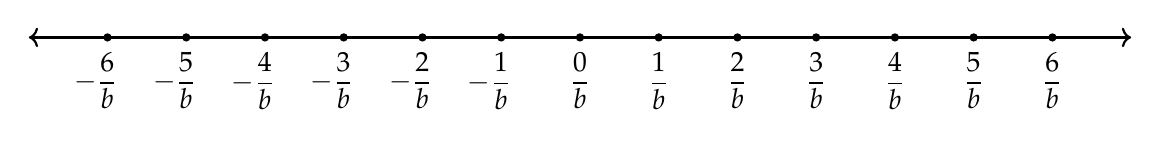
\begin{tikzpicture}
    \draw[<->,thick] (-7,0)--(7,0);
	\foreach \x in {-6,-5,-4,-3,-2,-1,0,1,2,3,4,5,6}
    {
    \fill (\x,0) circle (1.5pt);
    }
    \node[] at (0,-0.55) {$\dfrac{0}{b}$};
    \node[] at (1,-0.55) {$\dfrac{1}{b}$};
    \node[] at (2,-0.55) {$\dfrac{2}{b}$};
    \node[] at (3,-0.55) {$\dfrac{3}{b}$};
    \node[] at (4,-0.55) {$\dfrac{4}{b}$};
    \node[] at (5,-0.55) {$\dfrac{5}{b}$};
    \node[] at (6,-0.55) {$\dfrac{6}{b}$};
    \node[] at (-1.15,-0.55) {$-\dfrac{1}{b}$};
    \node[] at (-2.15,-0.55) {$-\dfrac{2}{b}$};
    \node[] at (-3.15,-0.55) {$-\dfrac{3}{b}$};
    \node[] at (-4.15,-0.55) {$-\dfrac{4}{b}$};
    \node[] at (-5.15,-0.55) {$-\dfrac{5}{b}$};
    \node[] at (-6.15,-0.55) {$-\dfrac{6}{b}$};
\end{tikzpicture}\]
Then, say
\[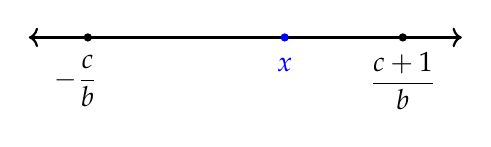
\begin{tikzpicture}
    \draw[<->,thick] (-2.75,0)--(2.75,0);
	\foreach \x in {-2,2}
    {
    \fill (\x,0) circle (1.5pt);
    }
    \node[] at (2,-0.55) {$\dfrac{c+1}{b}$};
    \node[] at (-2.15,-0.55) {$-\dfrac{c}{b}$};
    \node[color=blue] at (0.5,-0.35) {$x$};
    \fill[color=blue] (0.5,0) circle (1.5pt);
\end{tikzpicture}\]
Between $c/b$ and $(c+1)/b$, choose the one closest to $x$ and define $a/b$ as such. So, 
\[\abs{x - \frac{a}{b}} \leq \frac{1}{2}\left(\text{length of $\left[\frac{a}{b},\frac{a+1}{b}\right]$}\right) = \frac{1}{2b}\]
\end{proof}
\vspace*{1em}
Sometimes, we have a far better deal\\[0.2em]
\emph{e.g.}\quad $\pi = 3.1415926$
\begin{itemize}
\item $a/b = 3.14 = 314/100 = 157/100$; $|\pi - a/b| \approx 0.00159$. Compared to $1/2b = 1/100 = 0.01$, it's $\sim 16\%$ off.
\item $a/b = 22/7 = 3.\overline{142857}$; $|\pi - a/b| \approx 0.0013$. Compared to $1/2b = 1/14 = 0.07$, it's only $\sim 2\%$ off.
\end{itemize}

Why do we care about this? To prove transcendence of numbers. For example, if we want to prove $\pi$ or $e$ is transcendental, then we have to show that for \emph{every} polynomial $P$ with integer coefficients, we must have $P(\pi),P(e) \neq 0$. That's a tall order, since there are infinitely such polynomials.\\
\\
One idea in transcendence theory, a rule of thumb, is that if you can approximate an irrational number $\alpha$ by rational (or algebraic) numbers very well, then $\alpha$ is likely to be transcendental.\\
\\
\emph{e.g.}\quad $e^x = 1 + x + \dfrac{x^2}{2!} + \dfrac{x^3}{3!} + \dfrac{x^4}{4!} + \cdots$. So,\\[-0.5em]
\[e = x + \dfrac{1}{2!} + \dfrac{1}{3!} + \dfrac{1}{4!} + \cdots\]
Terms in the series decrease very rapidly, since $n!$ increases rapidly as $n\to \infty$.
\vspace*{2em}

\begin{definition}
Let $a/b$ and $c/d$ be (reduced) fractions. The \emph{mediant} of $a/b$ and $c/d$ is
\[\dfrac{a}{b} \vee \dfrac{c}{d} \coloneqq \dfrac{a+c}{b+d}\]
\emph{e.g.}\quad $\dfrac{5}{3} \vee \dfrac{11}{17} = \dfrac{5+11}{3 + 17} = \dfrac{16}{20}$.
\end{definition}

\vspace*{1em}

\begin{proposition}
Let $a/b$ and $c/d$ be reduced fractions, then $a/b \vee c/d$ lies between $a/b$ and $c/d$.
\end{proposition}
\begin{proof}
Plot $(b,a)$ and $(d,c)$ in the Cartesian plane, say we get
\[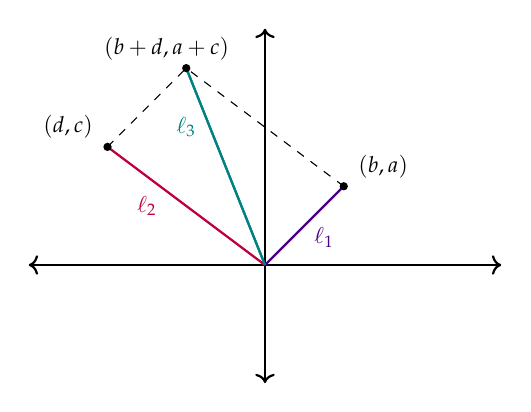
\begin{tikzpicture}
    \draw[<->,thick] (-3,0)--(3,0);
	\draw[<->,thick] (0,-1.5)--(0,3);
	\draw[-,thick,color=indigo] (0,0)--(1,1);
	\draw[-,thick,color=purple] (0,0)--(-2,1.5);
	\draw[-,thick,color=teal] (0,0)--(-1,2.5);
	\draw[-,thick,color=teal] (0,0)--(-1,2.5);
	\draw[-,dashed] (-2,1.5)--(-1,2.5);	
	\draw[-,dashed] (1,1)--(-1,2.5);	
	\fill (-2,1.5) circle (1.5pt);
    \fill (1,1) circle (1.5pt);
    \fill (-1,2.5) circle (1.5pt);
    \node[] at (1.5,1.25) {\footnotesize $(b,a)$};
    \node[] at (-2.5,1.75) {\footnotesize $(d,c)$};
    \node[] at (-1.25,2.75) {\footnotesize $(b+d,a+c)$};
    \node[color=teal] at (-1,1.75) {\footnotesize $\ell_3$};
    \node[color=purple] at (-1.5,0.75) {\footnotesize $\ell_2$};
    \node[color=indigo] at (0.75,0.35) {\footnotesize $\ell_1$};
\end{tikzpicture}\]
Then note that
\begin{align*}
\frac{a}{b} &\text{ is the slope of {\color{indigo} $\ell_1$}}\\[0.5em]
\frac{c}{d} &\text{ is the slope of {\color{purple} $\ell_2$}}\\[0.5em]
\frac{a+c}{b+d} &\text{ is the slope of {\color{teal} $\ell_3$}}
\end{align*}
Therefore, as a rational number, $\dfrac{a}{b}\vee \dfrac{c}{d} = \dfrac{a+c}{b+d}$ lies between $\dfrac{a}{b}$ and $\dfrac{c}{d}$.
\end{proof}

\vspace*{1em}

\begin{definition}
Let $a/b$ be a reduced fraction; in particular $b>0$. The \emph{Ford circle atop $a/b$} is the circle of diameter $1/b^2$ that is above and tangent to the real line at the rational number $a/b$.
\[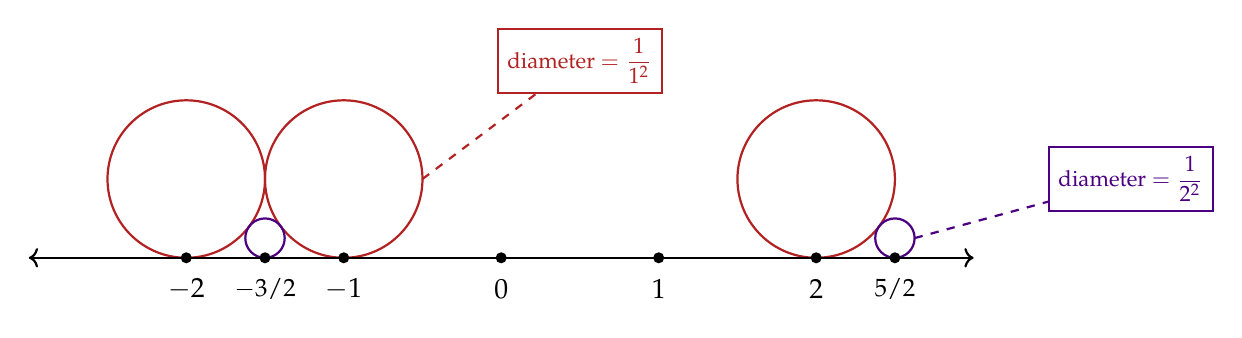
\begin{tikzpicture}[scale=2]
    \draw[thick,color=firebrick](-2,0.5) circle (0.5);
    \draw[thick,color=firebrick](-1,0.5) circle (0.5);
    \draw[thick,color=indigo](-1.5,0.125) circle (0.125);
    \draw[thick,color=firebrick](2,0.5) circle (0.5);
    \draw[thick,color=indigo](2.5,0.125) circle (0.125);
    \draw[<->,thick] (-3,0)--(3,0);
    \foreach \x in {-2,-1,0,1,2,2.5,-1.5}
    {
    \fill (\x,0) circle (1pt);
    }
    \node[] at (0,-0.2) {$0$};
    \node[] at (1,-0.2) {$1$};
    \node[] at (2,-0.2) {$2$};
    \node[] at (-1,-0.2) {$-1$};
    \node[] at (-2,-0.2) {$-2$};
    \node[] at (-1.5,-0.2) {\small $-3/2$};
    \node[] at (2.5,-0.2) {\small $5/2$};
    \node[draw,color=firebrick,thick](A) at (0.5,1.25) {\footnotesize diameter $=\dfrac{1}{1^2}$};
    \node[draw,color=indigo,thick](B) at (4,0.5) {\footnotesize diameter $=\dfrac{1}{2^2}$};
    \draw[dashed,color=firebrick,thick] (-0.5,0.5)--(A);
    \draw[dashed,color=indigo,thick] (2.625,0.125)--(B);
\end{tikzpicture}\]
Note that some Ford circles are tangent to each other.
\end{definition}

\vspace*{0.5in}

\subsection{Problems}
\vspace{0.1in}

\begin{problem}\label{Problem 6.1}\hfill
\begin{itemize}
\item[(a)] Find a nonzero rational polynomial $P(T)$ that has $\sqrt{5} + \sqrt[3]{7}$ as a root.
\item[(b)] Prove that $\sqrt{5} + \sqrt[3]{7}$ is irrational.
\item[(c)] Prove that if $p$ and $q$ are distinct prime numbers, then $\sqrt{p} + \sqrt{q}$ is irrational.
\end{itemize}
\end{problem}

\vspace*{0.1in}

\begin{problem}\label{Problem 6.2}
Consider the \emph{Fibonacci numbers}\footnote{This is an example of problematic naming in Number Theory. Fibonacci aka Leonardo Bonacci \emph{introduced} this sequence to the West in the 13th century but this sequence had been described earlier by Indian mathematicians, for example, as early as 200 BCE.}, define recursively by
\[F_0 = 0,\ F_1 = 1\ \text {and }\ F_n = F_{n-1} + F_{n-2}\ \text{ for all $n\geq 2$;}\]
so the first few terms are $0,\,1,\,1,\,2,\,3,\,5,\,8,\,13,\,\ldots$\\[0.5em]
For all $n\geq 2$, define $r_n = F_n/F_{n-1}$; so the first few terms are
\[\frac{1}{1},\,\frac{2}{1},\,\frac{3}{2},\,\frac{5}{3},\,\frac{8}{5}\,\ldots.\]
\begin{itemize}
\item[(a)] Prove that for all $n\geq 4,\ r_n = r_{n-1} \vee r_{n-2}$.
\item[(b)] Prove that the sequence $r_n$ converges (to a real number).
\item[(c)] Prove that $r_n$ converges to the \emph{golden ratio}:
\[\phi = \frac{1 + \sqrt{5}}{2}\]
\end{itemize}
For this problem, you can use any result that you may have seen in your Calculus classes.
\end{problem}

%\vspace*{0.1in}

\begin{problem}\label{Problem 6.3}
Using the Taylor expansion of $e^x$, we obtain
\[e = 1 + 1 + \frac{1}{2!} + \frac{1}{3!} + \cdots + \frac{1}{n!} + \cdots\]
In this problem, you will prove that $e$ is irrational.
\begin{itemize}
\item[(a)] Let $\displaystyle s_n \coloneqq \sum_{k=0}^n \frac{1}{k!}$, the $n^{\text{th}}$ term of the sequence of partial sums. Prove that
\[0 \leq e - s_n \leq \frac{1}{n}\cdot \frac{1}{n!}\]
\item[(b)] Assume $e$ is rational, and say $e = p/q$. Apply the previous result to $n = q$ and arrive at a contradiction.
\end{itemize}
\end{problem}

\vspace*{0.1in}

\begin{problem}\label{Problem 6.4}
Using Problem \ref{problem 4.5}, prove that for all positive integers $n$, we have
\[\sigma_1(n) \leq n \ln(n+1) + \gamma n;\]
where $\gamma$ is the Euler-Mascheroni constant.
\end{problem}
\newpage

\section{Lecture 7 (10/14)}
\vspace*{1em}

\begin{definition}
Let $a/b$ and $c/d$ be reduced fractions that are distinct as rational numbers. Then we say $a/b$ \emph{kisses} $c/d$ if $ad - bc = \pm 1$. Notationally
\[\frac{a}{b} \kiss \frac{c}{d}\qquad \text{if and only if}\quad \det\begin{pmatrix}
a & b\\ c& d
\end{pmatrix} = \pm 1\]
\end{definition}

\vspace*{1em}

\begin{proposition}\label{redkiss}
If $a/b$ kisses any fraction $c/d$ at all, then $\gcd(a,b) = 1$.
\end{proposition}
\begin{proof}
By assumption, $ax+ by = \pm 1$ has an integer solution: $(d,-c)$. Therefore $\gcd(a,b)\mid \pm 1$ and hence $\gcd(a,b) = 1$, necessarily.
\end{proof}

\vspace*{1em}

\begin{theorem}
Let $a/b$ and $c/d$ be fractions such that $b,d>0$. Then
\[\frac{a}{b}\kiss \frac{c}{d}\ \text{if and only if Ford circles atop $\dfrac{a}{b}$ and $\dfrac{c}{d}$ are tangent to each other.}\]
\end{theorem}
\begin{proof}
Let's set things up by first considering the Ford circles, say
\[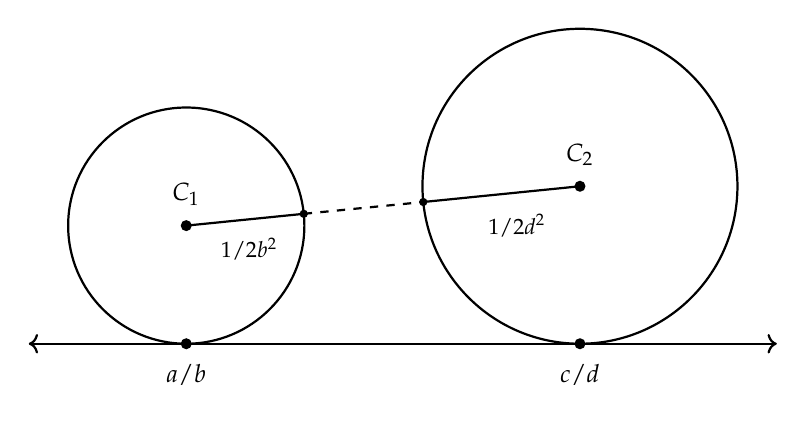
\begin{tikzpicture}[scale=2]
    \draw[thick](1,1) circle (1);
    \fill (1,1) circle (1pt);
    \fill (0.005,0.9) circle (0.75pt);
    \draw[thick](-1.5,0.75) circle (0.75);
    \fill (-1.5,0.75) circle (1pt);
    \fill (-0.7537,0.825) circle (0.75pt);
    \draw[<->,thick] (-2.5,0)--(2.25,0);
    \draw[dashed,thick] (-0.7537,0.825)--(0.005,0.9);
    \draw[thick] (0.005,0.9)--(1,1);
    \draw[thick] (-1.5,0.75)--(-0.7537,0.825);
    \foreach \x in {1,-1.5}
    {
    \fill (\x,0) circle (1pt);
    }
    \node[] at (1,-0.2) {\small $c/d$};
    \node[] at (-1.5,-0.2) {\small $a/b$};
    \node[] at (1,1.2) {\small $C_2$};
    \node[] at (-1.5,0.95) {\small $C_1$};
    \node[] at (-1.1,0.6) {\footnotesize $1/2b^2$};
    \node[] at (0.6,0.75) {\footnotesize $1/2d^2$};
\end{tikzpicture}\]
where $C_1$ and $C_2$ are the centres of the Ford circles atop $a/b$ and $c/d$ respectively.
\begin{align*}
\text{Cartesian coordinates of } C_1 &= \left(\dfrac{a}{b},\dfrac{1}{2b^2}\right)\\[0.5em]
\text{Similarly, cartesian coordinates of } C_2 &= \left(\dfrac{c}{d},\dfrac{1}{2d^2}\right)
\end{align*}
By Pythagoras' theorem (equivalently the distance formula)
\begin{align*}\label{smthng}
\overline{C_1C_2}^2 &= \left(\frac{1}{2b^2} - \frac{1}{2d^2}\right)^2 + \left(\frac{a}{b} - \frac{c}{d}\right)^2\\[0.5em]
&= \left(\frac{ad-bc}{bd}\right)^2 + \left(\frac{1}{2b^2} - \frac{1}{2d^2}\right)^2\tag{1}
\end{align*}
The Ford circles are tangent to each other if and only if
\begin{align*}
\overline{C_1C_2} &= \frac{1}{2b^2} + \frac{1}{2d^2}\\[0.5em]
\iff\overline{C_1C_2}^2 &= \left(\frac{1}{2b^2} + \frac{1}{2d^2}\right)^2\\[0.5em]
\underset{\refp{smthng}}{\iff}\left(\frac{ad-bc}{bd}\right)^2 + \left(\frac{1}{2b^2} - \frac{1}{2d^2}\right)^2 &= \left(\frac{1}{2b^2} + \frac{1}{2d^2}\right)^2\\[0.5em]
\iff\left(\frac{ad-bc}{bd}\right)^2 &= \left(\frac{1}{2b^2} + \frac{1}{2d^2}\right)^2 - \left(\frac{1}{2b^2} - \frac{1}{2d^2}\right)^2\\[0.5em]
\iff\left(\frac{ad-bc}{bd}\right)^2 &= 4\left(\frac{1}{2b^2}\right)\left(\frac{1}{2d^2}\right)\\[0.5em]
\iff(ad-bc)^2&= 1\\[0.5em]
\iff ad-bc&= \pm 1
\end{align*}
if and only if $\dfrac{a}{b}\kiss \dfrac{c}{d}$.
\end{proof}

\vspace*{1em}

\begin{proposition}\label{medsand}
Let $a/b$ be a reduced fraction. Then 
\begin{itemize}
\item[(1)] $a/b$ kisses infinitely many fractions.
\item[(2)] If $b>1$, then there are exactly two reduced fractions $c/d$ and $c'/d'$, with $d,d'<b$, that kiss $a/b$ such that $c/d \vee c'/d' = a/b$ and $c/d\kiss c'/d'$. 
\end{itemize}
\end{proposition}
\begin{proof}
\hfill
\begin{itemize}
\item[(1)] By assumption, $\gcd(a,b) = 1$. So, if $u/v$ is a reduced fraction kissing $a/b$, then by definition, $(x,y) = (v,u)$ is a solution to the equation
\[ax - by = \pm 1\]
We can take, without loss of generality, the equation $ax - by = 1$. Since $\gcd(a,b) = 1 = ax + (-b)y$, by Theorem \ref{ldea}, all solutions to this equation are of the form
\[u_n = u_0 + an,\quad v_n = v_0 + bn\qquad \text{(since $\lcm(a,-b) = -ab$)}\]
for any $n\in \zz$, where $(u_0,v_0)$ is a particular solution we obtain using the division algorithm.\\[1em]
There's at most one $n$ such that $v_n = 0$ since $b>0$. Whenever $v_n \neq 0$, $u_n/v_n$ or $-u_n/-v_n$ is a reduced fraction that kisses $a/b$.\\[1em]
Hence, there are infinitely many $u/v$'s that kiss $a/b$.\qed
\item[(2)] We have $b > 1$; let's plot the values of $\set{v_0 + bn}_{n \in \zz}$, say
\[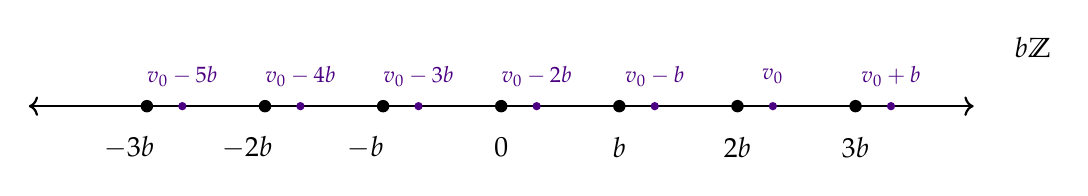
\begin{tikzpicture}[scale=1.5]
    \draw[<->,thick] (-4,0)--(4,0);
	\foreach \x in {-3,-2,-1,0,1,2,3}
    {
    \fill (\x,0) circle (1.5pt);
    }
    \foreach \y in {3.3,2.3,1.3,0.3,-0.7,-1.7,-2.7}
    {
    \fill[color=indigo] (\y,0) circle (1pt);
    }
    \node[] at (0,-0.35) {$0$};
    \node[] at (1,-0.35) {$b$};
    \node[] at (2,-0.35) {$2b$};
    \node[] at (3,-0.35) {$3b$};
    \node[] at (-1.15,-0.35) {$-b$};
    \node[] at (-2.15,-0.35) {$-2b$};
    \node[] at (-3.15,-0.35) {$-3b$};
    \node[] at (4.5,0.5) {$b\zz$};
    \node[color=indigo] at (2.3,0.25) {\footnotesize $v_0$};
    \node[color=indigo] at (3.3,0.25) {\footnotesize $v_0 + b$};
    \node[color=indigo] at (1.3,0.25) {\footnotesize $v_0-b$};
    \node[color=indigo] at (0.3,0.25) {\footnotesize $v_0-2b$};
    \node[color=indigo] at (-0.7,0.25) {\footnotesize $v_0-3b$};
    \node[color=indigo] at (-1.7,0.25) {\footnotesize $v_0-4b$};
    \node[color=indigo] at (-2.7,0.25) {\footnotesize $v_0-5b$};
\end{tikzpicture}\]
Where could $v_0$ lie? We cannot have $v_0 = nb$ for any $n \in \zz$, since the fact $av_0 - bu_0 = 1$ gives us $b = (an - u_0) = a(nb) - bu_0 = 1$, that is, $b\mid 1$. This is isn't possible as $b > 1$. Hence $v_0 \in (kb,(k+1)b)$ for some integer $k$.\\
\\
Therefore, among $\set{v_0 + bn}_{n \in \zz}$, \emph{exactly one} falls in $(0,b)$ and \emph{exactly one} falls in $(-b,0)$. Let $v_m \in \set{v_0 + bn}_{n \in \zz}$ be the one in $(0,b)$; we can then also consider $u_m$.\\
\\
Then $u_m/v_m \kiss a/b$ and $0<v_m<b$, so define $c/d \coloneqq u_m/v_m$. Furthermore, also define $c'/d' \coloneqq (a - u_m)/(b-v_m)$, then $d' < b$ and
\[\frac{c}{d} \vee \frac{c'}{d'} = \frac{c+c'}{d+d'} = \frac{a}{b}\]
by constriction. Lastly, note that
\begin{align*}
cd' - c'd &= u_m(b-v_m) - (a-u_m)v_m\\[0.5em]
&= (bu_m - av_m) + (u_mv_m - u_mv_m)\\[0.5em]
&= -1
\end{align*}
Thus, $c/d \kiss c'/d'$.\qed
\end{itemize}\renewcommand{\qedsymbol}{}
\vspace*{-\baselineskip}
\end{proof}

\vspace*{1em}

\begin{corollary}[geometric form]
Let $a/b$ be a reduced fraction. Then
\begin{itemize}
\item[(1)] The Ford circle atop $a/b$ has infinitely many Ford circles tangent to it.
\[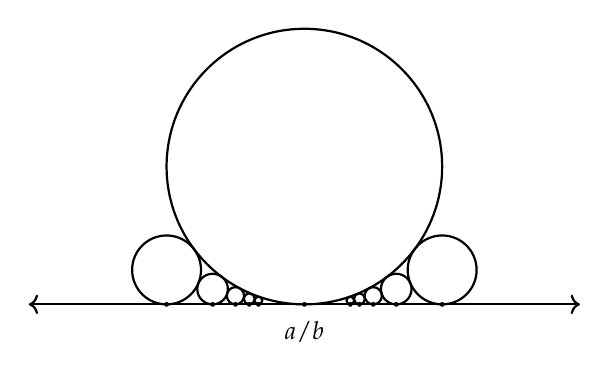
\begin{tikzpicture}[scale=3.5]
    \draw[thick](-2,0.5) circle (0.5);
    \draw[thick](-1.5,0.125) circle (0.125);
    \draw[thick](-1.66666,0.0555) circle (0.0555);
    \draw[thick](-1.75,0.03125) circle (0.03125);
    \draw[thick](-1.8,0.02) circle (0.02);
    \draw[thick](-1.8333,0.013889) circle (0.013889);
    \draw[thick](-2.5,0.125) circle (0.125);
    \draw[thick](-2.333,0.0555) circle (0.0555);
    \draw[thick](-2.25,0.03125) circle (0.03125);
    \draw[thick](-2.2,0.02) circle (0.02);
    \draw[thick](-2.1666,0.013889) circle (0.013889);
    \draw[<->,thick] (-3,0)--(-1,0);
    \foreach \x in {-2,-1.5,-1.66666,-1.75,-1.8,-1.8333,-2.5,-2.333,-2.25,-2.2,-2.1666}
    {
    \fill (\x,0) circle (0.25pt);
    }
    \node[] at (-2,-0.1) {\small $a/b$};
\end{tikzpicture}\]
\item[(2)] If $b>1$, then among the infinitely many Ford circles as above, there are exactly two whose mediant is the Ford circle atop $a/b$.
\[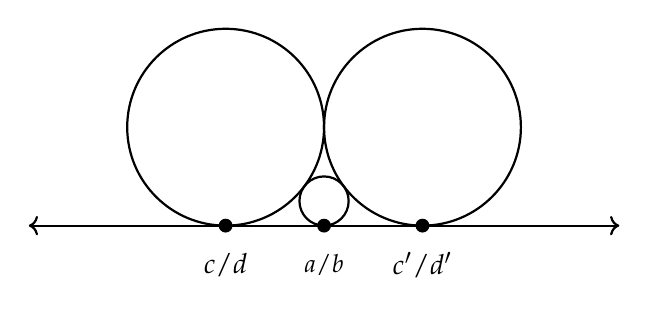
\begin{tikzpicture}[scale=2.5]
    \draw[thick](-2,0.5) circle (0.5);
    \draw[thick](-1,0.5) circle (0.5);
    \draw[thick](-1.5,0.125) circle (0.125);
    \draw[<->,thick] (-3,0)--(0,0);
    \foreach \x in {-2,-1,-1.5}
    {
    \fill (\x,0) circle (1pt);
    }
    \node[] at (-1,-0.2) {$c'/d'$};
    \node[] at (-2,-0.2) {$c/d$};
    \node[] at (-1.5,-0.2) {\small $a/b$};
\end{tikzpicture}\]
\end{itemize}
\end{corollary}

\vspace*{1em}

\begin{example}
Find the two kissing (reduced) fractions whose mediant is $83/71$.
\end{example}
\begin{proof}[Answer]
If $x/y$ was one of them, then $71x - 83y = \pm 1$. Let's employ the division algorithm
\begin{align*}
83 &= 71(1) + 12\\[0.5em]
71 &= 12(5) + 11\\[0.5em]
12 &= 11(1) + 1\\[0.5em]
11 &= 1(11) + 0
\end{align*}
Running this backwards, we get $1 = 71 (-7) + 83 (6)$ and so $-1 = 71(7) - 83(6)$.\\
\\
Take $\dfrac{c}{d} = \dfrac{7}{6}$, note $6 < 71$, and $\dfrac{c'}{d'} = \dfrac{83-7}{71-6} = \dfrac{76}{65}$.
\end{proof}

\vspace*{1em}

\begin{example}[in-class]
Find the two kissing (reduced) fractions $a/b$ and $c/d$ whose mediant is $15/32$.
\end{example}

\vspace*{1em}

\begin{theorem}
Consider the following process
\begin{itemize}
\item \emph{Step I.} Start with fractions $\dfrac{n}{1}$ as $n$ runs through the integers.
\item \emph{Step II.} Whenever you see two kissing fractions, form their mediant.
\item \emph{Step III.} Keep repeating \emph{Step II}.
\end{itemize}
Then
\begin{itemize}
\item[(1)] The fractions occurring in this sequence are reduced.
\item[(2)] Conversely, all reduced fractions occur in this sequence.
\end{itemize}
\end{theorem}
\begin{proof}
We induct on the the denominator of $a/b$, where $a/b$ is an element of the sequence.
\begin{itemize}
\item[(1)] For $b = 1$, $a/1$ is reduced.\\[0.5em]
Assume the inductive hypothesis; if $\dfrac{a}{b}\kiss \dfrac{c}{d}$, we form $\dfrac{a}{b}\vee \dfrac{c}{d} = \dfrac{a+c}{b+d}$.
\vspace*{0.2in}
\begin{subproof}
\vspace*{-0.1in}
\begin{lemma}\label{medkiss}
Suppose $\dfrac{x}{y} \kiss \dfrac{z}{w}$, then $\left(\dfrac{x}{y}\vee \dfrac{z}{w}\right)\kiss \dfrac{x}{y},\dfrac{z}{w}$.
\end{lemma}
\begin{proof}
We verify directly; since $x/y \kiss z/w$, i.e. $xy - yz = \pm 1$, note that
\begin{align*}
w(x+z) - z(y+w) &= xw + wz - yz - wz\\[0.5em]
&= xw - yz = \pm 1
\end{align*}
Therefore $\dfrac{x}{y}\vee \dfrac{z}{w} = \dfrac{x+z}{y+z} \kiss \dfrac{z}{w}$; similarly $\left(\dfrac{x}{y}\vee \dfrac{z}{w}\right) \kiss \dfrac{x}{y}$.
\end{proof}
\end{subproof}
%\vspace*{0.2in}
Now, since $\left(\dfrac{a}{b}\vee \dfrac{c}{d}\right) \kiss \dfrac{a}{b}$, the mediant is reduced by Proposition \ref{redkiss}.\qed

\item[(2)] If $b = 1$, then $\dfrac{a}{1}$ occurs in the base step.\\
\\
Assume the inductive hypothesis; now $b > 1$, therefore by Proposition \ref{medsand} there exist reduced fractions $c/d$ and $c'/d'$ with $d,d' < b$ such that 
\[\dfrac{c}{d} \vee \dfrac{c'}{d'} = \dfrac{a}{b}\]
$c/d$ and $c'/d'$ occur in the sequence by the inductive hypothesis. Therefore, so does $a/b$ as their mediant.\qed
\end{itemize}\renewcommand{\qedsymbol}{}
\vspace*{-\baselineskip}
\end{proof}

\vspace*{1em}

\begin{theorem}[Dirichlet's Approximation Theorem]
Let $x$ be an irrational real number. Then there exist infinitely many reduced fractions $a/b$ such that
\[\abs{x- \frac{a}{b}} < \frac{1}{2b^2}\]
\end{theorem}
\begin{proof}
\emph{I.} Start with $b=1$, $x$ is in the shadow of exactly Ford circle atop $\dfrac{a}{1}$
\[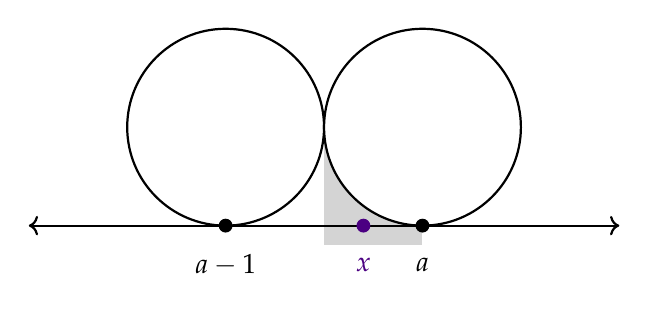
\begin{tikzpicture}[scale=2.5]
    \draw[thick](-2,0.5) circle (0.5);
    \draw [draw=none, fill=lightgrey] (-1.5,-0.1) rectangle (-1,0.5);
    \draw[thick,black,fill=white](-1,0.5) circle (0.5);
    \draw[<->,thick] (-3,0)--(0,0);
    \foreach \x in {-2,-1}
    {
    \fill (\x,0) circle (1pt);
    }
    \node[] at (-1,-0.2) {$a$};
    \node[] at (-2,-0.2) {$a-1$};
    \fill[color=indigo] (-1.3,0) circle (1pt);
    \node[color=indigo] at (-1.3,-0.2) {$x$};
\end{tikzpicture}\]
But then
\[\abs{x - \frac{a}{1}} < \frac{1}{2}\]
\vspace*{0.5em}\\
\emph{II.} Consider a Ford circle atop $a/b$ which shadows $x$.
\[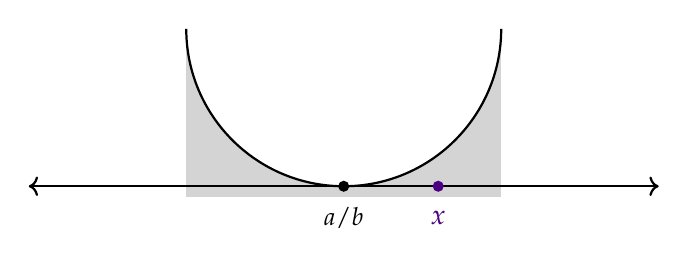
\begin{tikzpicture}[scale=4]
%    \draw[thick](-2,0.5) circle (0.5);
    \draw [draw=none, fill=lightgrey] (-1.5,-0.035) rectangle (-2.5,0.45);
    \draw[thick,black,fill=white] (-1.5,0.5) (-2.5,0.5) arc(0:180:-0.5);
    \draw[<->,thick] (-3,0)--(-1,0);
    \fill (-2,0) circle (0.5pt);
    \node[] at (-2,-0.1) {\small $a/b$};
    \fill[color=indigo] (-1.7,0) circle (0.5pt);
    \node[color=indigo] at (-1.7,-0.1) {$x$};
\end{tikzpicture}\]
Since $x$ is an irrational real number, so either $x>a/b$ or $x< a/b$. Let's treat the case $x > a/b$.\\
\begin{subproof}
{\bf Claim.} \emph{There exists a reduced fraction $\dfrac{c}{d}>\dfrac{a}{b}$ such that $d\leq b$ and $\dfrac{c}{d}\kiss \dfrac{a}{b}$}
\begin{proof}[Proof of Claim]
If $b = 1$, take $\dfrac{c}{d} = \dfrac{a+1}{1}$.\\
\\
If $b>1$, then by Proposition \ref{medsand} we can find reduced fractions $x/y$ and $x'/y'$ with $y,y'<b$ such that $a/b$ is their mediant. Let $c/d$ be one of these fractions that lies to the right of $a/b$ and by Lemma \ref{medkiss} we know that $c/d \kiss a/b$.
\end{proof}
\vspace*{0.005em}
\end{subproof}
\vspace*{0.5em}
\begin{minipage}{0.4\textwidth}
Consider the chain
\vspace*{0.3em}
\begin{align*}
\frac{a}{b} \vee \frac{c}{d} &= \frac{e}{f}\\[0.5em]
\frac{a}{b} \vee \frac{e}{f} &= \frac{g}{h}\\[0.1em]
\quad\vdots
\end{align*}
\end{minipage}
\begin{minipage}{0.6\textwidth}
\[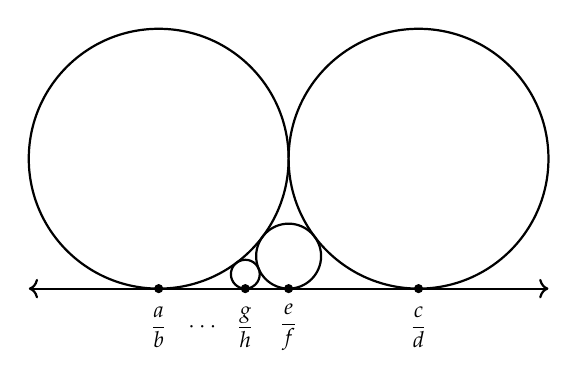
\begin{tikzpicture}[scale=3.3]
    \draw[thick](-2,0.5) circle (0.5);
    \draw[thick](-1,0.5) circle (0.5);
    \draw[thick](-1.5,0.125) circle (0.125);
    \draw[thick](-1.66666,0.0555) circle (0.0555);
%    \draw[thick](-1.75,0.03125) circle (0.03125);
%    \draw[thick](-1.8,0.02) circle (0.02);
%    \draw[thick](-1.8333,0.013889) circle (0.013889);
    \draw[<->,thick] (-2.5,0)--(-0.5,0);
%    \foreach \x in {-2,-1.5,-1.66666,-1.75,-1.8,-1.8333}
    \foreach \x in {-2,-1.5,-1.66666,-1}
    {
    \fill (\x,0) circle (0.5pt);
    }
    \node[] at (-2,-0.15) {\footnotesize $\dfrac{a}{b}$};
    \node[] at (-1,-0.15) {\footnotesize $\dfrac{c}{d}$};
    \node[] at (-1.5,-0.15) {\footnotesize $\dfrac{e}{f}$};
    \node[] at (-1.66666,-0.15) {\footnotesize $\dfrac{g}{h}$};
    \node[] at (-1.825,-0.15) {\footnotesize $\cdots$};
\end{tikzpicture}\]
\end{minipage}
\vspace*{0.5em}\\
The shadows of all these Ford circles cover the right shadow under $a/b$. So, at least one of the Ford circles in the chain must shadow $x$. Let's call the rational number this Ford circle is atop $a_1/b_1$, where $b_1 < b$.
\[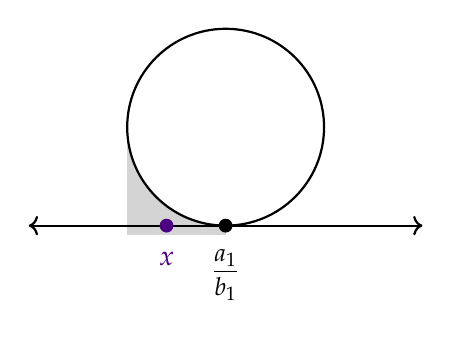
\begin{tikzpicture}[scale=2.5]
    \draw [draw=none, fill=lightgrey] (-1.5,-0.05) rectangle (-1,0.5);
    \draw[thick,black,fill=white](-1,0.5) circle (0.5);
    \draw[<->,thick] (-2,0)--(0,0);
    \foreach \x in {-1}
    {
    \fill (\x,0) circle (1pt);
    }
    \node[] at (-1,-0.25) {\small $\dfrac{a_1}{b_1}$};
    \fill[color=indigo] (-1.3,0) circle (1pt);
    \node[color=indigo] at (-1.3,-0.17) {$x$};
\end{tikzpicture}\]
The radius of the circle $=\dfrac{1}{2}(\text{diameter}) = \dfrac{1}{2b_1^2}$. So,
\[\abs{x - \frac{a_1}{b_1}}<\frac{1}{2b_1^2}\]
The case $x< a/b$ is similar (everything happens on the left). The theorem follows by starting with \emph{I.} and repeatedly applying \emph{II.}
\end{proof}

\vspace*{1em}

\begin{remark}[Warning/Clarification]
The theorem doesn't imply that this approximation works for \emph{every} integer $b$.\\[0.5em]
\emph{e.g.}\quad $\pi = 3.1415926\ldots$\\[0.5em]
For $b = 1$, we have $\abs{\pi - 3} < \dfrac{1}{2}$.\\[1em]
For $b = 2$, we cannot find an $\dfrac{a}{2}$ such that \[\abs{\pi - \dfrac{a}{2}}<\dfrac{1}{2\cdot 2^2}.\] Because the smallest fraction of this form is $\dfrac{7}{2} = 3.5$ and $\abs{\pi - 3.5} \approx 0.36$ while $\dfrac{1}{2\cdot 2^2} = 0.125$.\\[1em]
But $b = 7$ works, take $\dfrac{a}{b} = \dfrac{22}{7}$.
\end{remark}

%\vspace*{0.5in}

\subsection{Problems}
\vspace{0.1in}

\begin{problem}\label{Problem 7.1}
Write a formula which describes all fractions that kiss $7/11$.
\end{problem}
\newpage

\section{Lecture 8 (10/19)}
\vspace*{1em}

{\bf Pythagorean Triples.}
\begin{definition}
Let $a,b,c$ be positive integers. Say $(a,b,c)$ is a Pythagorean triple if $a^2 + b^2 = c^2$.
\[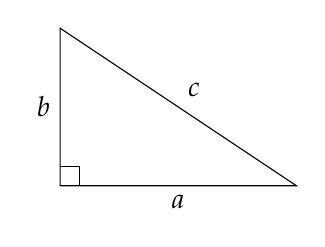
\begin{tikzpicture}
        \draw[]  (0, 0) coordinate (A) 
        -- node[left] {$b$} (0,2) coordinate (C) 
        -- node[above right] {$c$} (3,0) coordinate (B) 
        -- node[below] {$a$}  (-0.007,0);
       \draw (0,7pt) -- ++(7pt,0) -- ++(0,-7pt);
      \end{tikzpicture}\]
\emph{e.g.}\quad $(3,4,5),\ (5,12,13)$
\end{definition}

\vspace*{1.5em}

{\bf Goal.} Find \emph{all} Pythagorean triples.

\vspace*{2em}

{\bf Geometric Strategy.} Start with equation
\[a^2 + b^2  = c^2\]
Dividing both sides by $c^2$, and letting $x \coloneqq a/c$ and $y \coloneqq b/c$. Then
\[x^2 + y^2 = 1\]
Since $a,b,c$ are positive integers, $x,y$ are rational and $(x,y)$ lies on the unit circle! In other words, any Pythagorean triple gives rise to a rational point (points with rational coordinates) on the unit circle.\\
\\
For such a point $(x,y)$, consider the line passing through $(x,y)$ and $(-1,0)$. What can you say about the slope of this line?
\[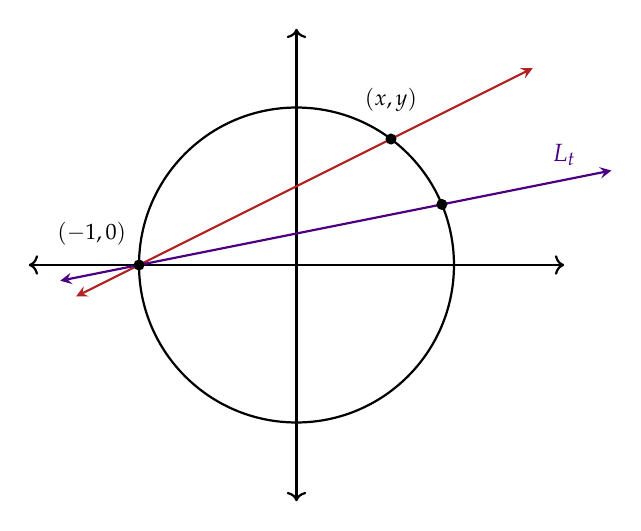
\begin{tikzpicture}[scale=2]
    \draw[<->,thick] (-1.7,0)--(1.7,0);
    \draw[<->,thick] (0,-1.5)--(0,1.5);
    \draw[thick](0,0) circle (1);
	\draw[<->,thick,>=stealth, color=firebrick] (-1.4,-0.2)--(1.5,1.25);   
	\draw[<->,thick,>=stealth, color=indigo] (-1.5,-0.1)--(2,0.6);   
    \fill (-1,0) circle (1pt);
    \fill (0.6,0.8) circle (1pt);
    \fill (0.923076923,0.384615385) circle (1pt);
    \node[] at (-1.3,0.2) {\footnotesize$(-1,0)$};
    \node[] at (0.6,1.05) {\footnotesize$(x,y)$};
    \node[] at (1.7,0.7) {\color{indigo} \small $L_t$};
\end{tikzpicture}\]
Suppose we draw a line $L_t$ through $(-1,0)$ with rational slop $t$, what we can say about the point at which it intersects the unit circle $C$?

\vspace*{1em}

\begin{proposition}
There's a bijection, where $P_0 = (-1,0)$
\[\begin{tikzcd}
\set{P = (x,y) \in \qq^2\ \Bigg\vert \begin{minipage}{0.13\textwidth}
\begin{center}
$P \neq P_0$\\[0.2em] $x^2 + y^2 = 1$
\end{center}
\end{minipage}}
 \arrow[r,shift left=2,"{\color{firebrick}f}"] &[1em]  \arrow[l,shift left=2,"{\color{indigo}g}"] \set{\begin{minipage}{0.2\textwidth}
\begin{center}
lines through $P_0$ with rational slope $t$.
\end{center}
\end{minipage}}
\end{tikzcd}\]
\end{proposition}
\begin{proof}
Define
\[{\color{firebrick}f}:P \mapsto \text{the line $L$ passing through $P_0$ and $P = (x,y)$}\]
Note that $L$ has rational slope: $\dfrac{y - 0}{x - (-1)} = \dfrac{y}{x+1}$ is rational since $x,y$ are rational numbers.\\
\\
We now describe ${\color{indigo}g}$: let $L_t$ be the line through $P_0$ with rational slop $t$. Then $L_t$ is defined by the equation \[y = t(x-(-1)) = t(x+1).\]
Let $(u,v) \in L_t \cap C$ then $v = t(u+1)$ and
\begin{align*}
u^2 + (t(u+1))^2 &= 1\\[0.5em]
u^2 + t^2(u^2 + 2u + 1) &= 1\\[0.5em]
(1+t^2)u^2 + 2ut^2 + (t^2 - 1) &= 0\\[0.5em]
u^2 + \left(\frac{2t^2}{1+t^2}\right)u + \left(\frac{t^2-1}{1+t^2}\right) &= 0
\end{align*}
As a quadratic equation in $u$, the equation above necessarily has two roots, say $\alpha$ and $\beta$. Crucial point is that $\alpha = -1$ is a root since $(-1,0) \in L_t\cap C$. Since we know that
\[\alpha\beta = \frac{t^2-1}{1+t^2},\quad \text{therefore }\ \beta = \frac{1-t^2}{1+t^2}\]
is the other root, i.e. $u = \dfrac{1-t^2}{1+t^2}$ is the $x$-coordinate of the other point in $L_t \cap C$. Then
\begin{align*}
v = t(u+1) &= t\left(\frac{1-t^2}{1+t^2} + 1\right)\\[0.5em]
&= \frac{2t}{1+t^2}
\end{align*}
Define ${\color{indigo}g}(L_t) = \left(\dfrac{1-t^2}{1+t^2},\dfrac{2t}{1+t^2}\right) \in \qq^2$.\\
\\[0.5em]
One readily checks $f$ and $g$ are inverses of each other.
\end{proof}

\emph{e.g.}\quad $t = 1/5$ corresponds to the Pythagorean triple $(12,5,13)$.
\begin{align*}
g(L_{1/5}) &= \left(\frac{1-(1/5)^2}{1+(1/5)^2},\frac{2(1/5)}{1+(1/5)^2}\right)\\[0.5em]
&= \left(\frac{24}{26},\frac{10}{26}\right) = \left(\frac{12}{13},\frac{5}{13}\right)
\end{align*}

%\vspace*{2.5em}

\begin{center}
{\Large Modular Arithmetic}
\end{center}

Sometimes, the remainder left after division can tell us a lot!
\begin{proof}[e.g.]\renewcommand{\qedsymbol}{}
\begin{itemize}
\item[(1)] Is $317 \times 694 = 219996$? \emph{No, since the last digit should be $8$. $317 \times 694 = 219998$.}
\end{itemize}
\begin{itemize}[leftmargin=4.4em]
\item[(2)] Is $9217$ a square of an integer? Equivalently, does $x^2 = 9217$ have an integer solution? \emph{No, because the last digit of a square can only be $0,1,4,5,6$ or $9$.}
\item[(3)] Does the equation 
\begin{align*}\label{intsol}
x^2 + y^2 &= 1234567 \tag{$\dagger$}
\end{align*}
have an integer solution?
\end{itemize}
\end{proof}

\begin{definition}
Let $m$ be a positive integer (called a \emph{modulus}). Say that two integers $a$ and $b$ are \emph{congruent modulo $m$}, written as
\[a\equiv b\modar{m},\]
if $m\mid (a-b)$, or equivalently $m\mid (b-a)$.\\
\\
Congruence modulo $m$ is an equivalence relation.
\end{definition}
\emph{e.g.} $317 \equiv 17\modar{10} \equiv 7\modar{10} \equiv -3\modar{10}$

\vspace*{1.5em}

\begin{proposition}\label{modps}
Let $m$ be a modulus, and $a,b,c,d$ are integers such that
\[a\equiv b\modar{m} \quad \text{and} \quad c\equiv d\modar{m}.\]
Then $a+c \equiv b+d\modar{m}$ and $ac \equiv bd\modar{m}$.
\end{proposition}
\begin{proof}
(product) By assumption, 
\begin{align*}
a-b &= mr,\quad \text{for some $r\in \zz$}; & c-d &= ms,\quad \text{for some $s\in \zz$}
\end{align*}
Then 
\begin{align*}
ac &= (b+mr)(d+ms)\\[0.5em]
&= bd + m^2rs + m(dr + bs)\\[0.5em]
ac - bd &= m(mrs + dr + bs)
\end{align*}
Therefore $m\mid (ac-bd)$, and hence $ac\equiv bd \modar{m}$.
\end{proof}

\vspace*{1em}

\begin{definition}
Let $x$ be an integer and $m$ a modulus, the \emph{natural representative of $x$ modulo $m$} is the remainder $r$ left under the division algorithm
\[x = qm + r,\quad 0 \leq r < m.\]
Therefore $x \equiv r\modar{m}$.
\end{definition}
\begin{proof}[e.g.]\renewcommand{\qedsymbol}{}
\begin{itemize}
\item[(1)] Compute the natural representative modulo $10$ of $1234567 \cdot 314159265$.\\[0.5em]
\hspace*{1.9em}\emph{Hard way:} Multiply this number and find out.\\[0.5em]
\hspace*{1.9em}\emph{Easy way:} Using Proposition \ref{modps},
\begin{align*}
1234567 \cdot 314159265 &\equiv 7\cdot 5\modar{10}\\[0.5em]
&\equiv 35\modar{10}\\[0.5em]
&\equiv 5\modar{10}
\end{align*}
\end{itemize}
\begin{itemize}[leftmargin=4.4em]
\item[(2)] Compute the natural representative modulo $13$ of $24^5$.\\[0.5em]
First, $24 = 13 + 11 \equiv 11\modar{13} \equiv -2\modar{13}$. Now, by Proposition \ref{modps},
\begin{align*}
28^5 \equiv (-2)^5\modar{13} &\equiv -32\modar{13}\\[0.5em]
&\equiv 39 - 32\modar{13}\\[0.5em]
&\equiv 7\modar{13}
\end{align*}
\item[(3)] Compute the natural representative modulo $7$ of $2^{10}$.\\
\\
(Attempt) $10 = 7 + 3\modar{7}$, and so
\[2^{10} \equiv 2^3\modar{7} \equiv 8\modar{7} \equiv 1\modar{7}\]
Incorrect! $2^{10} \not\equiv 2^3\modar{7}$.\\
\\
(Actual) $2\equiv 2\modar{7},\ 2^2\equiv 4\modar{7},\ 2^3\equiv 8\modar{7}\equiv 1\modar{7}$. So, 
\[2^{10} = 2^3\cdot 2^3\cdot 2^3\cdot 2\equiv 1\cdot 1\cdot 1\cdot 2 2\modar{7}\equiv 2\modar{7}\]
\emph{Caution.} In general, $b \equiv c\modar{m}$ does \emph{not} imply $a^b\equiv a^c\modar{m}$.
\end{itemize}
\end{proof}

%\vspace*{1em}

\begin{proposition}
Let $N$ be a positive integer, and $S$ be the sum of its digits. Then $N \equiv S\modar{9}$, and hence also $N \equiv S\modar{3}$.
\end{proposition}
\begin{proof}
Let $N = d_0 + d_1\cdot 10 + \cdots + d_k\cdot 10^k$, e.g. $247 = 7 + 4\cdot 10 + 7\cdot 100$. Then
\begin{align*}
N &= d_0 + d_1\cdot 10 + \cdots + d_k\cdot 10^k\\[0.5em]
&\equiv d_0 + d_1\cdot 1 + \cdots + d_k\cdot 1^k\modar{9},\quad\text{by Proposition \ref{modps}}\\[0.5em]
&\equiv d_0 + d_1 + \cdots + d_k\modar{9}\\[0.5em]
&\equiv S\modar{9}\\[-3em]
\end{align*}
\end{proof}
\emph{e.g.}\quad Note $247 \equiv 2 + 4 + 7 \modar{9} \equiv 13\modar{9} \equiv 1 + 3\modar{9} \equiv 4\modar{9}$.

\vspace*{3em}

Back to example \refp{intsol}. Does the equation $x^2 + y^2 = 1234567$ have an integer solution?
\begin{proof}[Answer]
Strategy is to look at the equation modulo $4$.
\begin{itemize}[leftmargin=*]
\item[] If $z$ is an even integer, then $z = 2n$ for some integer $n$, and so 
\[z^2 = (2n)^2 = 4n^2 \equiv 0\modar{4}\]
\item[] If $z$ is an odd integer, then $z = 2m+1$ for some integer $m$, and so 
\[z^2 = (2m+1)^2 = 4m^2 + 4m + 1 \equiv 1\modar{4}\]
\end{itemize}
Therefore, if a solution $(x,y)$ existed then $x,y \equiv 0,1\modar{4}$ and so $x^2 + y^2 \equiv 0,1,2\modar{4}$.\\
\\
But 
\begin{align*}
1234567 &= 12345\cdot 100 + 67\\[0.5em]
&\equiv 67\modar{4}\\[0.5em]
&\equiv 64 + 3\modar{4}\\[0.5em]
&\equiv 3\modar{4}
\end{align*}
Thus, no solution exists.
\end{proof}

\vspace*{2em}

{\bf Solving Quadratic Equations, so far.}
\begin{itemize}[itemsep = 2em]\label{quadeqex}
\item[(1)] $x^2 + y^2 = 1234567$ has no integer solutions.
\item[(2)] $x^2 + y^2 = z^2$ has infinitely many integer solutions, since we found all the rational solutions to the equation $X^2 + Y^2 = 1$.
\[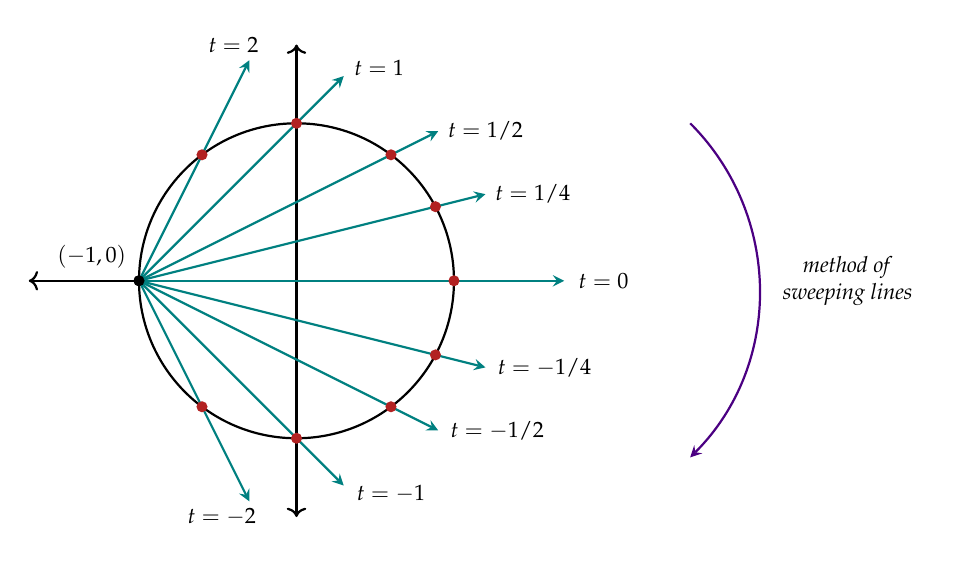
\begin{tikzpicture}[scale=2]
    \draw[<-,thick] (-1.7,0)--(-1,0);
    \draw[<->,thick] (0,-1.5)--(0,1.5);
    \draw[thick](0,0) circle (1);
    \fill (-1,0) circle (1pt);
	\draw[->,thick,>=stealth, color=teal] (-1,0)--(-0.3,1.4); %t = 2
    \fill[color=firebrick] (-0.6,0.8) circle (1pt); %t = 2
    \draw[->,thick,>=stealth, color=teal] (-1,0)--(0.3,1.3); %t = 1
    \fill[color=firebrick] (0,1) circle (1pt); %t = 1
    \draw[->,thick,>=stealth, color=teal] (-1,0)--(0.9,0.95); %t = 1/2
    \fill[color=firebrick] (0.6,0.8) circle (1pt); %t = 1/2
    \draw[->,thick,>=stealth, color=teal] (-1,0)--(1.2,0.55); %t = 1/4
    \fill[color=firebrick] (0.882352941,0.470588235) circle (1pt); %t = 1/4
    \draw[->,thick,>=stealth, color=teal] (-1,0)--(1.7,0); %t = 0
    \fill[color=firebrick] (1,0) circle (1pt); %t = 0
	\draw[->,thick,>=stealth, color=teal] (-1,0)--(-0.3,-1.4); %t = -2
    \fill[color=firebrick] (-0.6,-0.8) circle (1pt); %t = -2
    \draw[->,thick,>=stealth, color=teal] (-1,0)--(0.3,-1.3); %t = -1
    \fill[color=firebrick] (0,-1) circle (1pt); %t = -1
    \draw[->,thick,>=stealth, color=teal] (-1,0)--(0.9,-0.95); %t = -1/2
    \fill[color=firebrick] (0.6,-0.8) circle (1pt); %t = -1/2
    \draw[->,thick,>=stealth, color=teal] (-1,0)--(1.2,-0.55); %t = -1/4
    \fill[color=firebrick] (0.882352941,-0.470588235) circle (1pt); %t = -1/4
    \fill (-1,0) circle (1pt);
	\node[] at (-1.3,0.15) {\footnotesize$(-1,0)$};
    \node[] at (-0.4,1.5) {\footnotesize $t=2$};
    \node[] at (-0.475,-1.5) {\footnotesize $t=-2$};
    \node[] at (0.525,1.35) {\footnotesize $t=1$};
    \node[] at (0.6,-1.35) {\footnotesize $t=-1$};
    \node[] at (1.2,0.95) {\footnotesize $t=1/2$};
    \node[] at (1.275,-0.95) {\footnotesize $t=-1/2$};
    \node[] at (1.5,0.55) {\footnotesize $t=1/4$};
    \node[] at (1.575,-0.55) {\footnotesize $t=-1/4$};
    \node[] at (1.95,0) {\footnotesize $t=0$};
	\draw[->,>=stealth,thick,color=indigo] (1.5,1) (2.5,1) arc(225:135:-1.5);
    \node[] at (3.5,0) {\footnotesize\begin{tabular}{c}\emph{method of}\\ \emph{sweeping lines}\end{tabular}};
\end{tikzpicture}\]
\item[(3)] Find all rational solutions to $x^2 + y^2 = 3$.
\begin{itemize}
\item[(i)] No obvious ``pivot" with rational coordinates.
\[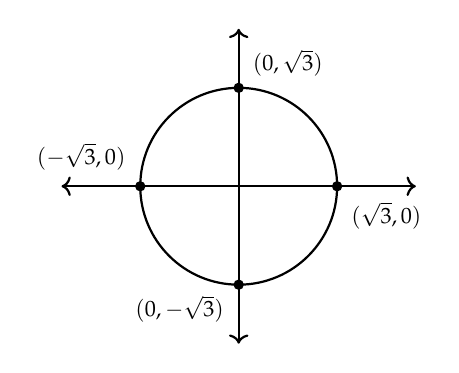
\begin{tikzpicture}[scale=1.25]
    \draw[<->,thick] (1.8,0)--(-1.8,0);
    \draw[<->,thick] (0,-1.6)--(0,1.6);
    \draw[thick](0,0) circle (1);
    \fill (-1,0) circle (1.5pt);
    \fill (1,0) circle (1.5pt);
    \fill (0,-1) circle (1.5pt);
    \fill (0,1) circle (1.5pt);
	\node[] at (-1.6,0.3) {\footnotesize$(-\sqrt{3},0)$};
	\node[] at (1.5,-0.3) {\footnotesize$(\sqrt{3},0)$};
	\node[] at (0.5,1.25) {\footnotesize$(0,\sqrt{3})$};
	\node[] at (-0.6,-1.25) {\footnotesize$(0,-\sqrt{3})$};
\end{tikzpicture}\]
\item[(ii)] Look at integer solutions.\\[0.5em]
Since $x^2,y^2 \geq 0$ and $x^2 + y^2 = 3$, necessarily $0 \leq x^2,y^2 \leq 3$. So, if $x,y \in \zz$, then $x,y = 0,\pm 1$. But none of these solve $x^2 + y^2 = 3$, and therefore there are no integer solutions\\[0.5em]
Alternatively, you can reduce mod $4$ and proceed as in (1).\\
\item[(iii)] How about rational solutions?\\[0.5em]
Assume towards a contradiction that $(u,v) \in \qq^2$ is a solution of $x^2 + y^2 = 3$, i.e.
\begin{align*}\label{eq81}
u^2 + v^2 = 3 \tag{$\star$}
\end{align*}
Let $c$ be the $\lcm$ of the denominators of $x$ and $y$ in their reduced form, and write
\begin{align*}\label{eq82}
u = \frac{a}{c},\quad v = \frac{b}{c} \tag{$\star\star$}
\end{align*}
{\small (\emph{e.g.} if $u = 3/10$ and $v = 4/15$, then $c = \lcm(10,15) = 30$; rewrite as $u = 9/30$ and $v = 8/30$.)}\\[0.5em]
Then $\gcd(a,b,c) = 1$ (see Problem \ref{Problem 8.1}) and $c\geq 1$.\\
\\
Rewriting \refp{eq81} using \refp{eq82}, we get
\begin{align*}\label{eq83}
\frac{a^2}{b^2} + \frac{b^2}{c^2} = 3 \iff a^2 + b^2 = 3c^2 \tag{$\star\star\star$}
\end{align*}
We want to now employ modular arithmetic, so for that a good modulus to choose will be $3$. Since $a,b,c \in \zz$, we get
\[a^2 + b^2 = 3c^2 \equiv 0 \modar{3}\]
Now, note that since $a \equiv 0,1,2\modar{3}$, therefore $a^2 \equiv 0,1\modar{3}$; similarly for $b^2\modar{3}$. Hence, the only way we have $a^2 + b^2 \equiv 0\modar{3}$ is if $a^2 \equiv b^2 \equiv 0\modar{3}$. Thus, $3\mid a^2$ and $3\mid b^2$, and so necessarily $3\mid a$ and $3\mid b$.\\
\\
Let $a = 3a_0$ and $b = 3b_0$, substituting this in \refp{eq83} gives us
\begin{align*}
3c^2 &= (3a_0)^2 + (3b_0)^2\\[0.5em]
c^2 &= 3(a_0^2 + b_0^2),\ \text{necessarily}
\end{align*}
Therefore $3\mid c^2$, and so necessarily $3\mid c$.\\
\\
Altogether we have $3\mid a,\,3\mid b$ and $3\mid c$; but we had $\gcd(a,b,c) = 1$. Hence we have arrived at a contradiction and thus $x^2 + y^2 = 3$ has no rational solutions.
\end{itemize}
\end{itemize}

\vspace*{0.5in}

\subsection{Problems}
\vspace{0.1in}

\begin{problem}\label{Problem 8.1}
Consider a pair of reduced fractions, $N_u/D_u$ and $N_v/D_v$ distinct as rational numbers. Let $c\coloneqq \lcm(D_u,D_v)$ and then suppose $c = D_um_u = D_vm_v$ for some integers $m_u,m_v$. Define $a = N_um_u$ and $b = n_vm_v$; prove that $\gcd(a,b,c) = 1$.
\end{problem}

\vspace{0.1in}

\begin{problem}\label{Problem 8.2}
Prove that there are infinitely many positive integer triples $(x,y,z)$ such that \[x^2 + 2y^2 = 3z^2.\]
{\footnotesize Hint: find an appropriate rational point that will act as a ``pivot", much like in the case of classifying Pythagorean triples that we saw in this lecture.}
\end{problem}

\vspace{0.1in}

\begin{problem}\label{Problem 8.3}
Let $N$ be a positive integer, and $A$ be the alternating sum of its digits. That is, if $N$ has a decimal expansion with units digit $u$, tens digit $t$, hundreds digit $h$ in units place, thousands digit $s$, then $A = u - t + h - s + \cdots$. Then $N \equiv S\modar{11}$.
\end{problem}

\vspace{0.1in}

\begin{problem}\label{Problem 8.4}\hfill
\begin{itemize}
\item[(a)] Let $n$ be any integer. Prove that $n^2$ is congruent to $0,\, 1$ or $4$ modulo $8$.
\item[(b)] Prove that there exists no integer solution $(x, y, z)$ to the equation
\[x^2 + y^2 + z^2 = 314159265358979323846264338327.\]
\item[(c)] Demonstrate that there are infinitely many positive integers that \emph{cannot} be written as a sum of three squares.
\end{itemize}
\end{problem}

\vspace{0.1in}

\begin{problem}\label{Problem 8.5}
Let $p$ be any prime number and let $a$ and $b$ be any two integers.
\begin{itemize}
\item[(a)] Prove that if $a \equiv b \modar{p}$, then $a^p \equiv b^p \modar{p^2}$.
\item[(b)] Prove that if $a \equiv b \modar{p}$, then $a^{p^2} \equiv b^{p^2} \modar{p^3}$.
\item[(b)] (challenge) Can you generalise?
\end{itemize}
\end{problem}

\vspace{0.1in}

\begin{problem}\label{Problem 8.6}
Compute (the natural representative of) $3^{10^{10^{10}}}\modar{7}$.
\end{problem}

\vspace{0.1in}

\begin{problem}\label{Problem 8.7}
Prove that a modulus $m$ is even if and only if there exists an integer $x$ such that $x \not\equiv 0\modar{m}$ and $x + x\equiv 0\modar{m}$.
\end{problem}

\vspace{0.1in}

\begin{problem}\label{Problem 8.8}
Recall the Fibonacci numbers from Problem \ref{Problem 6.2}. Prove that for all $n\geq 1$,
\[F_n \equiv 4^{n-1}(2^n - 1)\modar{11}\]
\end{problem}
\newpage

\section{Lecture 9 (10/21)}
\vspace*{1em}

{\bf Notation.} Let $m$ be a modulus. By $\zz/m$ or $\zz/m\zz$ we mean the set of equivalence classes of integers with respect to the following (equivalence) relation
\[a \sim b \iff a \equiv b \modar{m}\]
For any $a \in \zz$, its equivalence class will be denoted as $\overline{a}$ or $[a]$.\\
\\
Essentially, $\overline{a}$ is the set that collects all integers that leave behind the same remainder as $a$ when divided by $m$, i.e. have the same natural representative modulo $m$ as $a$. Note that $\overline{a} = \overline{r}$, where $r$ is the natural representative of $a$ modulo $m$.\\
\\
\emph{e.g.}\quad $m = 2,\ a = 1$, \[\overline{1} = \set{\ldots,-3,-1,1,3,5,\ldots} = \setp{1 + 2n}{n \in \zz}\]
$m = 5,\, a = 7$, 
\[\overline{7} = \set{\ldots,-8,-3,2,7,12,17,\ldots} = \overline{2} = \setp{2 + 5n}{n \in \zz}\]
\\
Proposition \ref{modps} can be recast as saying \emph{addition and multiplication are well-defined operations on $\zz/m\zz$} (i.e., $\zz/m\zz$ is a ring).

\vspace*{2.5em}

{\bf Division of integers modulo $m$.}
\begin{itemize}
\item[(1)] With $\qq,\, \rr$ or $\cc$, we can divide by any non-zero number to solve linear equations. Consider, for example, $(2 + 3i)z = 5$; then
\begin{align*}
z= \frac{5}{2+3i}&= \frac{5}{2+3i}\cdot\frac{2 - 3i}{2 - 3i}\\[0.5em]
&= \frac{5(2 - 3i)}{(2+3i)(2 - 3i)}\\[0.5em]
&= \frac{10 - 15i}{2^2 + 3^2} = \frac{10}{13} - \frac{15}{13}i
\end{align*}
\item[(2)] With $\zz$, division can be tricky: $3x = 5$ has no integer solutions, but $3x = 6$ has $x = 2$ as a solution.
\item[(3)] When can we divide in $\zz/m\zz$?
\end{itemize}

\vspace*{2em}

\begin{definition}
Let $m$ be a modulus and $a$ an integer. Say that $b \in \zz$ is a \emph{multiplicative inverse of $a$ modulo $m$} if
\[ab \equiv 1\modar{m}\]
\emph{e.g.}\quad $m = 11$ and $a = 4$. Then $b = 2$ is \emph{not} a multiplicative inverse of $a$, since \[ab = 8 \not\equiv 1 \modar{11}.\]
But $b = 3$ is, because $ab = 12 \equiv 1 \modar{11}$.\\
\\
In fact, any other integer $c$ such that $ac \equiv 1\modar{11}$ will be of the form $3 + 11n$. 
%Since, 
%\[c \equiv 12c \equiv 3(ac) \equiv 3\modar{11}\]
\end{definition}

\vspace*{1em}

When $a$ has a multiplicative inverse $b$ modulo $m$, we can solve linear equations of the form
\[ax \equiv c \modar{m}\]
easily.\\
\\
Multiply by $b$, and you get $(ba)x \equiv bc\modar{m}$. Since $ba \equiv 1 \modar{m}$, we obtain $x \equiv (ba)x \equiv bc \modar{m}$.\\
\\
\emph{e.g.} Let's solve $4x \equiv 7\modar{11}$. We found $b = 3$ is a multiplicative inverse of $4$ modulo $11$, therefore
\[x \equiv (3\cdot 4)x \equiv 3\cdot (4x) \equiv 3\cdot 7\equiv 21 \equiv 10\modar{11}\]
So, when does a given integer have a multiplicative inverse with respect to a given modulus?

\vspace*{1.5em}

\begin{theorem}\label{modinv}
Let $m$ be a modulus and $a$ an integer. Then
\begin{itemize}
\item[(1)] $a$ has a multiplicative inverse modulo $m$ if and only if $\gcd(a,m) = 1$.
\item[(2)] When $a$ has a multiplicative inverse modulo $m$, then any two multiplicative inverses are necessarily congruent modulo $m$. That is, they define the same equivalence class in $\zz/m\zz$.
\end{itemize}
\end{theorem}
\begin{proof}\hfill
\begin{itemize}
\item[(1)] ($\Rightarrow$) Say $b$ is the multiplicative inverse of $a$ modulo $m$, that is $ab \equiv 1 \modar{m}$. So, $m\mid (ab - 1)$ and therefore $ab - 1 = mx$ for some $x\in \zz$. Hence $ab + m(-x) = 1$, and thus $\gcd(a,m)\mid 1$; so $\gcd(a,m) = 1$, necessarily.\\
\\
($\Leftarrow$) Suppose $\gcd(a,m) = 1$, then by B\'ezout's Identity there exist $x,y \in \zz$ such that $ax + my = 1$. Therefore $ax \equiv 1 \modar{m}$, and hence $x$ is a multiplicative inverse of $a$ modulo $m$.
\item[(2)] Say $b$ and $b'$ are two multiplicative inverses of $a$ modulo $m$, then
\[b = b\cdot 1\equiv b(ab')\equiv (ba)b' \equiv 1\cdot b' \equiv b'\modar{m}\]\\[-5em]
\end{itemize}
\end{proof}

\vspace*{0.5em}

\begin{example}[in-class]\hfill
\begin{itemize}
\item[(1)] Find the multiplicative inverse of $15$ modulo $37$.
\item[(2)] Using (1), solve the linear equation/congruence $15x \equiv 4\modar{37}$.
\end{itemize}
\end{example}

\vspace*{1em}

\begin{corollary}
$\overline{a}$ has a \emph{unique} multiplicative inverse $\overline{b}$ in $\zz/m\zz$ if and only if $\gcd(a,m) = 1$.
\end{corollary}

\vspace*{1em}

\begin{corollary}\label{cancel}
If $\gcd(a,m) = 1$, then for any $x,y \in \zz$,
\[ax\equiv ay\modar{m} \implies x\equiv y \modar{m}\]
\end{corollary}

\vspace*{1em}

\begin{corollary}\label{primeinv}
Let $p$ be a prime number and $a \in \zz$. Then $a$ has a multiplicative inverse modulo $p$ if and only if $p\nmid a$ if and only if $\overline{a} \neq \overline{0}$ in $\zz/p\zz$. $\zz/p\zz$ is a field!
\end{corollary}

\vspace*{2.5em}

\begin{center}
{\Large Modular Dynamics}
\end{center}

Dynamics in the simplest mathematical form (discrete time): Let $X$ be a set and $f:X \to X$ a function, what happens in this sequence $x_0,\,f(x_0),\,f(f(x_0)),\,f(f(f(x_0))),\ldots, f^n(x_0),\ldots$?\\
\\
\emph{e.g.}\quad Consider $X = \nn = \zz_+ = \set{1,2,\ldots}$, let $f:\nn \to \nn$ be defined as
\[f(n) = \begin{cases}n/2 & \text{$n$ is even}\\[0.5em] 3n+1 & \text{$n$ is odd} \end{cases}\]\\
Say $x_0 = 17$, then the sequence reads: $17,\ 52,\ 26,\ 13,\ 40,\ 20,\ 10,\ 5,\ 16,\ 8,\ 4,\ 2,\ 1,\ 4,\ 2,\ 1,\ldots$
\[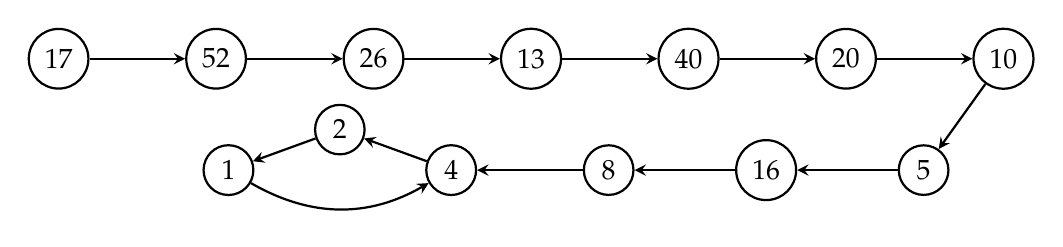
\begin{tikzpicture}[->,>=stealth,auto,node distance=2cm,
  thick,main node/.style={circle,draw}]

  \node[main node] (1) {$17$};
  \node[main node] (2) [right of=1] {$52$};
  \node[main node] (3) [right of=2] {$26$};
  \node[main node] (4) [right of=3] {$13$};
  \node[main node] (5) [right of=4] {$40$};
  \node[main node] (6) [right of=5] {$20$};
  \node[main node] (7) [right of=6] {$10$};
  \node[main node] (8) [below left of=7,xshift=0.4cm] {$5$};
  \node[main node] (9) [left of=8] {$16$};
  \node[main node] (10) [left of=9] {$8$};
  \node[main node] (11) [left of=10] {$4$};
  \node[main node] (12) [above left of=11,yshift=-0.9cm] {$2$};
  \node[main node] (13) [below left of=12,yshift=0.9cm] {$1$};
%  \node (7) [right of=6] {$\cdots$};

  \path[every node/.style={font=\sffamily\small}]
    (1) edge[] node[] {} (2)
    (2) edge[] node[] {} (3)
    (3) edge[] node[] {} (4)
    (4) edge[] node[] {} (5)
    (5) edge[] node[] {} (6)
    (6) edge[] node[] {} (7)
    (7) edge[] node[] {} (8)
    (8) edge[] node[] {} (9)
    (9) edge[] node[] {} (10)
    (10) edge[] node[] {} (11)
    (11) edge[] node[] {} (12)
    (12) edge[] node[] {} (13)
    (13) edge[bend right] node[] {} (11);
\end{tikzpicture}\]

%\vspace*{1em}

\begin{conjecture}[Collatz, $3n+1$]
For any $x_0 \in \nn$, there exists a $n>0$ such that $f^n(x_0) = 1$.
\end{conjecture}

\vspace*{2em}

{\bf Modular Dynamics.} $X = \zz/m\zz$ or some subset of $\zz/m\zz$.\\
\\
{\bf Additive Modular Dynamics.}\\[0.2em]
For a modulus $m$ and an integer $a$, we consider the dynamics of the function
\[\fbox{$+a\modar{m}$}:\zz/m\zz \to \zz/m\zz,\quad \overline{x} \mapsto \overline{x + a}\]\\
\emph{e.g.} Let $X = \zz/21\zz,\ a = 6$. We consider the dynamics of \fbox{$+6\modar{21}$} with $x_0 = 2$,
\[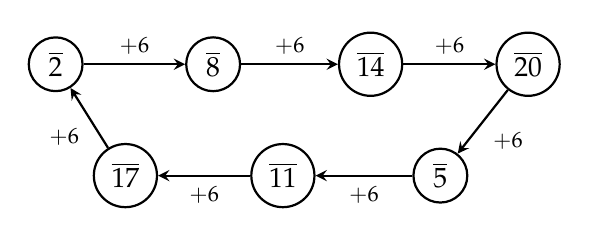
\begin{tikzpicture}[->,>=stealth,auto,node distance=2cm,
  thick,main node/.style={circle,draw}]

  \node[main node] (1) {$\overline{2}$};
  \node[main node] (2) [right of=1] {$\overline{8}$};
  \node[main node] (3) [right of=2] {$\overline{14}$};
  \node[main node] (4) [right of=3] {$\overline{20}$};
  \node[main node] (5) [below left of=4,xshift=0.3cm] {$\overline{5}$};
  \node[main node] (6) [left of=5] {$\overline{11}$};
  \node[main node] (7) [left of=6] {$\overline{17}$};

%  \path[every node/.style={font=\sffamily\small}]
%    (1) edge[bend left] node[above] {} (2)
%    (2) edge[bend left] node[above] {} (3)
%    (3) edge[bend left] node[above right] {} (4)
%    (4) edge[bend left] node[below right] {} (5)
%    (5) edge[bend left] node[below] {} (6)
%    (6) edge[bend left] node[below] {} (7)
%    (7) edge[bend left] node[left] {} (1);
\path[every node/.style={font=\sffamily\small}]
	(1) edge[] node[] {\footnotesize $+6$} (2)
	(2) edge[] node[] {\footnotesize $+6$} (3)
	(3) edge[] node[] {\footnotesize $+6$} (4)
    (4) edge[] node[] {\footnotesize $+6$} (5)
    (5) edge[] node[] {\footnotesize $+6$} (6)
    (6) edge[] node[] {\footnotesize $+6$} (7)
    (7) edge[] node[] {\footnotesize $+6$} (1);
\end{tikzpicture}\]
this is a \emph{cycle} of \emph{length} $7$.

\vspace*{1em}

\begin{proposition}
Let $m$ be a modulus and let $a$ be an integer. Then the dynamics of \fbox{$+a\modar{m}$} consists of $\gcd(a,m)$-many cycles of length $\ell = m/\gcd(a,m)$.
\end{proposition}
\begin{proof}
Suppose we start with $\overline{b} \in \zz/m\zz$
\[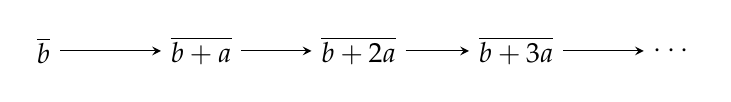
\begin{tikzpicture}[->,>=stealth,auto,node distance=2cm,main node/.style={rectangle,draw}]

  \node[] (1) {$\overline{b}$};
  \node[] (2) [right of=1] {$\overline{b+a}$};
  \node[] (3) [right of=2] {$\overline{b+2a}$};
  \node[] (4) [right of=3] {$\overline{b+3a}$};
  \node[] (5) [right of=4] {$\cdots$};

  \path[every node/.style={font=\sffamily\small}]
    (1) edge[] node[] {} (2)
    (2) edge[] node[] {} (3)
    (3) edge[] node[] {} (4)
    (4) edge[] node[] {} (5);
\end{tikzpicture}\label{cycle1}\tag{$\ast$}\]
In step $k$, we get $\overline{b + ka}$.\\
\\
Because $X = \zz/m\zz$ is a finite set, we return to $\overline{b}$ eventually (e.g. when $k = m$). Let $\ell$ be the smallest positive integer such that
\[\overline{b} = \overline{b + \ell a}\label{cycle2}\tag{$\ast\ast$}\]
and $\ell$ is necessarily the length of the cycle \refp{cycle1}.\\
\\
Rewriting \refp{cycle2}, we get $b \equiv b + \ell a\modar{m}$; equivalently, $\ell a \equiv 0 \modar{m}$. That is, $m\mid \ell a$ and $\ell$ is the smallest positive integer with this property. Therefore $\ell a = \lcm(a,m)$, and hence
\[\ell = \frac{\lcm(a,m)}{a} = \frac{m}{\gcd(a,m)}\]
So, the number of cycles $= m/\ell = \gcd(a,m)$.
\end{proof}

\vspace*{1.5em}

\begin{corollary}
If $\gcd(a,m) = 1$, then \fbox{$+a\modar{m}$} on $\zz/m\zz$ has just \emph{one} cycle of length $m$.
\end{corollary}

\vspace*{0.5in}

\subsection{Problems}
\vspace{0.1in}

\begin{problem}\label{Problem 9.1}\hfill
\begin{itemize}
\item[(1)] Find the multiplicative inverse of $15$ modulo $49$.
\item[(2)] Using (1), solve the linear equation/congruence $15x \equiv 8\modar{49}$.
\end{itemize}
\end{problem}

\vspace*{0.1in}

\begin{problem}\label{Problem 9.2}
Solve the congruences $5x \equiv 11\modar{37}$ and $11y \equiv 5\modar{37}$. If solutions exist, simplify $xy\modar{37}$.
\end{problem}

\vspace{0.1in}

\begin{problem}\label{Problem 9.3}
Consider the following modular dynamical system, which is neither additive nor multiplicative.
\begin{itemize}
\item[(a)] Let $X = \zz/13\zz$ and let $f : X \to X$ be given by
\[x \mapsto f(x) \coloneqq x^2 + 3 \modar{13}.\]
Draw the complete diagram for the dynamics of $f$.
\item[(b)] Let $A_0 = 0$ and let $A_{n+1} = f(A_n) \modar{13}$ for all integers $n \geq 0$. What is $A_{2021} \modar{13}$?
\end{itemize}
\end{problem}
\newpage

\section{Lecture 10 (10/26)}
\vspace*{1em}

{\bf Multiplicative Modular Dynamics.}\\[0.2em]
\emph{First complication:} unlike additive modular dynamics, \fbox{$\times a\modar{m}$} is not reversible.\\[0.3em]
\emph{e.g.} \[\fbox{$\times 12 \modar{20}$}:\zz/20\zz \to \zz/20\zz,\quad \overline{n} \mapsto \overline{12n}\] is \emph{not} reversible (bijective). Since, $12x\equiv 1 \modar{20}$ doesn't have a solution as $\gcd(12,20) = 4 \neq 1$.

\vspace*{1em}

\begin{definition}
Let $m$ be a modulus. We define the following set
\[\Phi(m) = \setp{i \in \zz}{0\leq i < m \text{ and }\gcd(i,m) = 1};\]
it's the set of natural representatives of integers that are multiplicatively invertible modulo $m$.\\
\\
We define the Euler's totient function $\varphi:\zz \to \cc$ as $\varphi(m) \coloneqq \card\Phi(m)$.
\end{definition}

\vspace*{0.2em}

\emph{e.g.} $\Phi(20) = \set{1,3,7,9,11,13,17,19}$, so $\varphi(20) = 8$.\\[1em]

We restate the existence of multiplicative inverse modulo $m$
\begin{proposition}
Let $a$ be an integer between $0$ and $m-1$ (if not, consider that integer's natural representative modulo $m$; which, by definition, is an integer between $0$ and $m-1$).\\[0.5em]
Then $a \in \Phi(m)$ if and only if $a$ has a multiplicative inverse modulo $m$ if and only if\ $\fbox{$\times a\modar{m}$}:\zz/m\zz \to \zz/m\zz$ is reversible (bijective).
\end{proposition}

\vspace*{1em}

\begin{proposition}
A modulus $m$ is prime if and only if $\varphi(m) = m-1$.
\end{proposition}
\begin{proof}
($\Rightarrow$) Suppose $m = p$ is prime, then $\Phi(p) = \set{1,\ldots,p-1}$ since any positive integer less than $p$ is necessarily coprime to it. Hence $\varphi(p) = \card\Phi(p) = p-1$.\\
\\
($\Leftarrow$) Suppose $\varphi(m) = m-1$. Note that $m \neq 1$, since if $m = 1$, then $m - 1 = 0$ but $\varphi(m) = \varphi(1) = \card\Phi(1) = \card\set{0} = 1$. Hence $0 \notin \Phi(m)$, as the only number coprime to $0$ is $1$ (see Problem \ref{gcd a} (i)). Now, we clearly have $\Phi(m) \subseteq \set{1,\ldots,m-1}$; furthermore, we've been given that $\card\Phi(m) = m - 1 = \card\set{1,\ldots,m-1}$. Therefore, necessarily, $\Phi(m) = \set{1,\ldots,m-1}$. Suppose $m$ wasn't prime, then there exists an integer $a$ such that $1< a < m$ and $a \mid m$. Hence $a \in \set{1,\ldots,m-1} = \Phi(m)$ but $\gcd(a,m) = a$, by Problem \ref{gcd a} (ii), contradicting the fact that $a \in \Phi(m)$. Thus, $m$ is necessarily prime. 
\end{proof}

\vspace*{1em}

\begin{proposition}
If $a,b \in \Phi(m)$, then there exists a unique $c \in \Phi(m)$ such that $ab \equiv c\modar{m}$. That is, $\Phi(m)$ is closed under multiplication modulo $m$).
\end{proposition}
\begin{proof}
Take $c$ to be the natural representative of $ab$ modulo $m$, that is, the remainder left when we divide $ab$ by $m$
\[ab = mq + c,\quad 0 \leq c < m\]
In particular, $ab \equiv c\modar{m}$. We need to now show that $\gcd(c,m) = 1$, we show this by producing a multiplicative inverse of $c$ modulo $m$; see Theorem \ref{modinv}.\\[1em]
Since $\gcd(a,m) = \gcd(b,m) = 1$, by Theorem \ref{modinv}, there exist multiplicative inverses of $a$ and $b$ modulo $m$, say $a'$ and $b'$ respectively. That is,
\[aa'\equiv 1 \modar{m}\quad \text{and} \quad bb'\equiv 1 \modar{m}.\]
Note that, 
\begin{align*}
c(a'b') &\equiv (ab)(a'b')\modar{m}\\[0.5em]
&\equiv (aa')(bb')\modar{m}\\[0.5em]
&\equiv 1\modar{m}
\end{align*}
Therefore $a'b'$ is a multiplicative inverse of $c$ modulo $m$, and hence $c\in \Phi(m)$. Its uniqueness follows from the uniqueness of the remainder in the division algorithm.
\end{proof}

\vspace*{1em}

{\bf Dynamics of \fbox{$\mathbold{\times a \modar{m}}$}, when $\mathbold{a\in \Phi(m)}$.}\\[1em] 
We focus on $X = \Phi(m)$. That is, we consider, for $a \in \Phi(m)$
\[\fbox{$\times a \modar{m}$}:\Phi(m) \to \Phi(m)\]

Let's start with an example, let's consider
\[\fbox{$\times 7 \modar{20}$}:\Phi(20) \to \Phi(20).\]
Note that $\Phi(20) = \set{1,3,7,9,11,13,17,19}$ and that $3$ is the multiplicative inverse of $7$ modulo $3$.\\[1em]
We see that we get
\[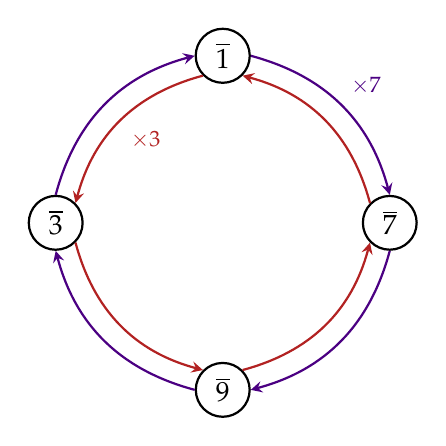
\begin{tikzpicture}[->,>=stealth,auto,node distance=3cm,
  thick,main node/.style={circle,draw}]

  \node[main node] (1) {$\overline{1}$};
  \node[main node] (2) [below right of=1] {$\overline{7}$};
  \node[main node] (3) [below left of=2] {$\overline{9}$};
  \node[main node] (4) [above left of=3] {$\overline{3}$};
\path[every node/.style={font=\sffamily\small}]
	(1.0) edge[indigo,bend left] node[] {\footnotesize$\times 7$} (2.90)
	(2.135) edge[firebrick,bend right] node[] {} (1.315)
	(2.270) edge[indigo,bend left] node[] {} (3.0)
	(3.45) edge[firebrick,bend right] node[] {} (2.225)
	(3.180) edge[indigo,bend left] node[] {} (4.270)
	(4.315) edge[firebrick,bend right] node[] {} (3.135)
  (4.90) edge[indigo,bend left] node[] {} (1.180)
  (1.225) edge[firebrick,bend right] node[] {\footnotesize$\times 3$} (4.45);
\end{tikzpicture}
\qquad\qquad
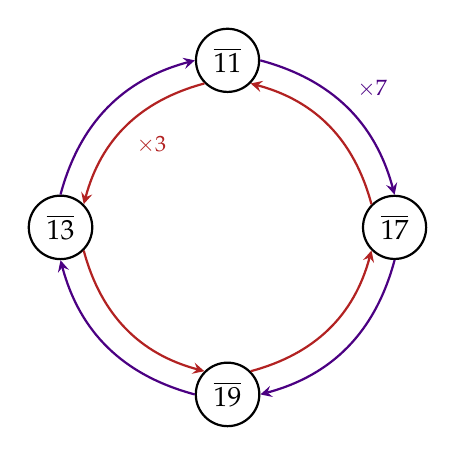
\begin{tikzpicture}[->,>=stealth,auto,node distance=3cm,
  thick,main node/.style={circle,draw}]

  \node[main node] (1) {$\overline{11}$};
  \node[main node] (2) [below right of=1] {$\overline{17}$};
  \node[main node] (3) [below left of=2] {$\overline{19}$};
  \node[main node] (4) [above left of=3] {$\overline{13}$};
\path[every node/.style={font=\sffamily\small}]
	(1.0) edge[indigo,bend left] node[] {\footnotesize$\times 7$} (2.90)
	(2.135) edge[firebrick,bend right] node[] {} (1.315)
	(2.270) edge[indigo,bend left] node[] {} (3.0)
	(3.45) edge[firebrick,bend right] node[] {} (2.225)
	(3.180) edge[indigo,bend left] node[] {} (4.270)
	(4.315) edge[firebrick,bend right] node[] {} (3.135)
  (4.90) edge[indigo,bend left] node[] {} (1.180)
  (1.225) edge[firebrick,bend right] node[] {\footnotesize$\times 3$} (4.45);
\end{tikzpicture}\]
Therefore, the dynamics of \fbox{$\times 7 \modar{20}$} in the set $\Phi(20)$ has $2$ cycles, each of length $4$.

\vspace*{2em}

\begin{lemma}\label{multcycle}
Let $m$ be a modulus and $a \in \Phi(m)$. Then the dynamics of
\[\fbox{$\times a \modar{m}$}:\Phi(m) \to \Phi(m)\]
consists of cycles, all of the same length.
\end{lemma}
\begin{proof}
Initialising the dynamics at $1$, we obtain a sequence of powers of $a$ modulo $m$
\[1,\ a,\ a^2,\ a^3,\,\ldots,\ a^n,\,\ldots\label{apow1}\tag{$\star$}\]
Since $\Phi(m)$ is a finite set, there must be repetition.\\[0.5em]
Say, $0\leq e<f$ are integers such that $a^f \equiv a^e \modar{m}$. Since $\gcd(a,m) = 1$, we necessarily have $\gcd(a^e,m) = 1$; rewriting the previous expression  as $a^e\cdot a^{f-e}\equiv a^e\modar{m}$, by Corollary \ref{cancel}, we obtain $a^{f-e}\equiv 1\modar{m}$.\\[0.5em]
Therefore, there's an integer $\ell = f-e>0$ such that $a^\ell \equiv 1\modar{m}$. Let $\ell_0$ be the smallest such positive integer.\\[0.5em]
\begin{subproof}
{\bf Claim.} \emph{If $e,f$ are integers such that $0\leq e < f < \ell_0$, then $a^e\not\equiv a^f\modar{m}$.}
\begin{proof}[Proof of Claim]
Suppose not, that is $e,f$ are integers as given but $a^e \equiv a^f\modar{m}$. Then similarly as before, by invoking Corollary \ref{cancel}, we obtain $a^{f-e} \equiv 1\modar{m}$. This contradicts the minimality of $\ell_0$, since $f-e < \ell_0 - e < \ell_0$, therefore $a^e\not\equiv a^f\modar{m}$.
\end{proof}
\vspace*{0.05em}
\end{subproof}
\vspace*{1em}
Thus, with this claim, we conclude that \refp{apow1} is a cycle of length $\ell_0$.\\
\\
Now, let $b \in \Phi(m)$ be arbitrary, and consider the sequence
\[b,\ ba,\ ba^2,\ ba^3,\,\ldots,\ ba^n,\,\ldots\label{apow2}\tag{$\star_b$}\]
Since $a^{\ell_0} \equiv 1\modar{m}$, necessarily $ba^{\ell_0} \equiv b\modar{m}$. Therefore, \refp{apow2} is a cycle of length less than or equal to $\ell_0$. Suppose the length of \refp{apow2} was $k < \ell_0$, that is, $ba^k \equiv b\modar{m}$. Then, since $\gcd(b,m) = 1$, by Corollary \ref{cancel} we obtain $a^k\equiv \modar{m}$. This contradicts the minimality of $\ell_0$, and hence \refp{apow2} must also have length $\ell_0$.
\end{proof}

\vspace*{0.5in}

\subsection{Problems}
\vspace{0.1in}

\begin{problem}\label{Problem 10.1}\hfill
\begin{itemize}
\item[(a)] Compute the length of the cycles in the dynamics of \fbox{$\times a \modar{8}$} for every $a \in \Phi(8)$. Compare the length with $\varphi(8)$.
\item[(b)] Compute the length of the cycles in the dynamics of \fbox{$\times 3 \modar{14}$}. Compare the length with $\varphi(14)$.
\end{itemize}
\end{problem}
\newpage

\section{Lecture 11 (10/28)}
\vspace*{1em}

\begin{theorem}[Euler-Fermat]\label{euler-fermat}
Let $m$ be a modulus and $a \in \Phi(m)$. Then
\[a^{\varphi(m)} \equiv 1\modar{m}\]
\end{theorem}
\begin{proof}
Consider the dynamics of \fbox{$\times a\modar{m}$} in $\Phi(m)$. We have seen in Lemma \ref{multcycle} that all cycles have the same length, say $\ell_0$. In particular, initialising at $1$ we obtain
\[a^{\ell_0} \equiv 1\modar{m}.\label{ef1}\tag{1}\]
One the other hand, let $c$ be the number of cycles in the dynamical system. Then, since $\card\Phi(m) = \varphi(m)$, necessarily
\[\varphi(m) = c\ell_0.\label{ef2}\tag{2}\]
Therefore, 
\[a^{\varphi(m)} \underset{\refp{ef2}}{=} (a^{\ell_0})^c \underset{\refp{ef1}}{\equiv} 1^c \equiv 1\modar{m}\]\\[-2em]
\end{proof}

\vspace*{1em}

\begin{corollary}[Fermat's little theorem]\label{fermatlittle}
Given a prime $p$, let $a\in \Phi(p)$, then
\[a^{p-1} \equiv 1\modar{p};\]
since $\varphi(p) = p-1$. If we rewrite the above expression as $a^p \equiv a\modar{p}$, this holds true even for $a = 0$.
\end{corollary}

\vspace*{1em}

\begin{example}
Simplify $2^{2021}\modar{9}$
\end{example}
\begin{proof}[Answer]
Note $\Phi(9) = \set{1,2,4,5,7,8}$; so $\varphi(9) = 6$ and therefore $2^6 \equiv 1\modar{9}$ since $\gcd(2,9) = 1$. Now, $2021 = 336\cdot 6 + 5$; so
\begin{align*}
2^{2021} &= (2^6)^{336}\cdot 2^5\\[0.5em]
&\equiv 2^5\modar{9}\\[0.5em]
&\equiv 5\modar{9}
\end{align*}
%\[2^{2021} = (2^6)^{336}\cdot 2^5 \equiv 2^5 \equiv 5\modar{9}\]
On the other hand, $3^6 = 9^3 \equiv 0\modar{9} \not\equiv 1\modar{9}$, since $\gcd(3,9) \neq 1$.
\end{proof}

\vspace*{1em}

\begin{corollary}
Let $m$ be a modulus and $a \in \Phi(m)$. Then, for any integer $b,c$ such that $b \equiv c \modar{\varphi(m)}$, we have
\[a^b \equiv a^c\modar{m}\]
\end{corollary}

\vspace*{2em}

{\bf Application: Primality Testing.} Given a number $N$, determine whether $N$ is a prime.\\
\\
One way is to find the prime factorisation of $N$, this is usually hard. A zero-knowledge approach is to see if there's an integer $0 < x < N$ such that $x\mid N$.

\vspace*{0.5em}

\begin{proposition}
Let $N\geq 3$, and suppose no integer $1 < x \leq \sqrt{N}$ divides $N$. Then $N$ must be prime.
\end{proposition}
\begin{proof}
We prove the contrapositive; suppose $N$ is composite. Then $N = ab$, where $1<a,b<N$. Without loss of generality, let $a\leq b$, then
\[a^2 \leq ab = N\]
Therefore, $1 < a \leq \sqrt{N}$. Hence, we have found an $a$ such that $1< a\leq \sqrt{N}$ and $a\mid N$.
\end{proof}

\vspace*{0.5em}

\emph{e.g.} If $N \sim 2^{2000}$, we only need to check for divisors upto $\sqrt{N} \sim 2^{1000}$.\\
\\[0.5em]
One consequence of Corollary \ref{fermatlittle} is that if, for some $1 < a < N$, we have $a^{N-1} \equiv 1\modar{N}$, then $N$ cannot be prime.\\[0.5em]
\emph{Caution: the converse is not true, there exist composite numbers $M$ such that $x^{M-1} \equiv 1\modar{M}$ for any integer $x$ coprime to $M$; for instance, $M = 561$. Such numbers are called \emph{Carmichael numbers} or (absolute) Fermat pseudoprimes.}

\vspace*{1.5em}

\begin{theorem}\label{totientform}
Let $n$ be a positive integer with prime factorisation $n = p_1^{e_1}p_2^{e_2}\cdots p_t^{e_t}$. Then 
\[\varphi(n) = n\left(1 - \frac{1}{p_1}\right)\left(1 - \frac{1}{p_2}\right)\cdots\left(1 - \frac{1}{p_t}\right)\]
\end{theorem}
\begin{proof}
Recall that $\varphi(n) = \card\Phi(n)$, where 
\[\Phi(n) = \setp{i \in \zz}{0 \leq i < n,\ \gcd(i,n) = 1}.\]
Consider the sets
\begin{align*}
A &= \set{0,1,\ldots,n-1}\\[0.5em]
B_1 &= \setp{a \in A}{p_1 \mid a}\\[0.5em]
B_2 &= \setp{a \in A}{p_2 \mid a}\\
&\qquad\quad \vdots\\
B_t &= \setp{a \in A}{p_t \mid a}
\end{align*}
Note that 
\begin{align*}
\Phi(n) &= \setp{a \in A}{p_i \nmid a,\ \text{for all $i = 1,\ldots,t$}}\\[0.5em]
&= \setp{a \in A}{a \notin B_i,\ \text{for all $i = 1,\ldots,t$}} = A\setminus \cup_{i = 1}^t B_i,
\end{align*}
so we need to compute \[\card\!\left(A\setminus \cup_{i = 1}^t B_i\right) = \card A - \card\!\left(\cup_{i = 1}^t B_i\right) = n - \card\!\left(\cup_{i = 1}^t B_i\right),\]
in particular $\card\left(\cup_{i = 1}^t B_i\right)$; which, by the inclusion – exclusion principle, is
\[\card\!\left(\bigcup_{i = 1}^t B_i\right) = \left(\sum_{k = 1}^t (-1)^{k+1}{\sum_{1\leq i_1 < \cdots < i_k \leq t}}\!\!\! \card\left(B_{i_1} \cap B_{i_2} \cap \cdots \cap B_{i_k}\right)\right)\]
For that, take any choice of indices $1 \leq i_1 < \cdots < i_k \leq t$ and we claim
\[\card\!\left(B_{i_1} \cap \cdots \cap B_{i_k}\right) = \frac{n}{p_{i_1}\cdots p_{i_k}}\]
Since the primes $p_1,\ldots,p_t$ are distinct, we have
\begin{align*}
B_{i_1} \cap \cdots \cap B_{i_k} &= \setp{a \in A}{p_{i_1}\mid a,\ldots, p_{i_k}\mid a}\\[0.5em]
&= \setp{a \in A}{p_{i_1}\cdots p_{i_k}\mid a}\\[0.5em]
&= \setp{p_{i_1}\cdots p_{i_k} b}{0 \leq b <  n/(p_{i_1}\cdots p_{i_k})}
\end{align*}
We explicitly prove the last equality; clearly the latter set is a subset of the former. Consider an element of the former, i.e., an $c \in A$ such that $p_{i_1}\cdots p_{i_k}\mid c$, then $c = p_{i_1}\cdots p_{i_k} d$, for some $d \in \zz$. Since $c \in A$, we have $0 \leq c = p_{i_1}\cdots p_{i_k} d < n$, which shows that $0 \leq d < n/(p_{i_1}\cdots p_{i_k})$. Therefore $c = p_{i_1}\cdots p_{i_k} d$ is an element of the latter set, and hence our equality of sets in the last step is justified.\\
\\
Hence $\card\!\left(B_{i_1} \cap \cdots \cap B_{i_k}\right) = \dfrac{n}{p_{i_1}\cdots p_{i_k}}$, as claimed.\\
\\
We return to our calculations,
\begin{align*}
\varphi(n) &= \card\Phi(n)\\[0.5em]
&= n - \left(\sum_{k = 1}^t (-1)^{k+1}{\sum_{1\leq i_1 < \cdots < i_k \leq t}}\!\!\! \card\!\left(B_{i_1} \cap B_{i_2} \cap \cdots \cap B_{i_k}\right)\right)\\[1em]
&= n - \left(\sum_{k = 1}^t (-1)^{k+1}{\sum_{1\leq i_1 < \cdots < i_k \leq t}}\ \frac{n}{p_{i_1}\cdots  p_{i_k}}\right)\\[1em]
&= n\left(1 - \left(\frac{1}{p_1} + \cdots + \frac{1}{p_2} \right) + \left(\sum_{1 \leq i_1 < i_2 \leq t}\frac{1}{p_{i_1}p_{i_2}}\right) + \cdots + (-1)^t\,\frac{1}{p_1\cdots p_t} \right)\\[1em]
&= n\left(1 - \frac{1}{p_1}\right)\left(1 - \frac{1}{p_2}\right)\cdots\left(1 - \frac{1}{p_t}\right)\\[0.1em]
\end{align*}
Hence $\varphi(n) = n\left(1 - \dfrac{1}{p_1}\right)\left(1 - \dfrac{1}{p_2}\right)\cdots\left(1 - \dfrac{1}{p_t}\right)$.
\end{proof}

\vspace*{1.5em}

\begin{corollary}
Let $p$ be a prime, then $\varphi(p^e) = p^{e-1}(p-1)$ for any integer $e \geq 1$.
\end{corollary}

\vspace*{1em}

\begin{corollary}
$\varphi$ is multiplicative. That is, for positive integers $a,b$ such that $\gcd(a,b) = 1$, we have
\[\varphi(ab) = \varphi(a)\varphi(b)\]
\end{corollary}

%\vspace*{1em}

\begin{example}[in-class]
Compute $\varphi(72)$, and then compute (the natural representative of) $5^{2403}\modar{72}$.
\end{example}

\vspace*{0.5in}

\subsection{Problems}
\vspace{0.1in}

\begin{problem}\label{Problem 11.1}
Compute (the natural representative of) $3^{10^{10^{10}}}\modar{7}$.
\end{problem}

\vspace{0.1in}

\begin{problem}\label{Problem 11.2}
A \emph{Sophie Germain prime} is a prime number $p$ such that $2p + 1$ is also a prime. For example, $p = 2, 3, 5$ are Sophie Germain primes, but $p = 7$ is not (since $15 = 2\cdot 7 + 1$ is not a prime).\\
\\
Prove that if $p$ is a Sophie Germain prime, then $2p + 1$ is a divisor either of $2^p - 1$ or of $2^p + 1$, but not of both.
\end{problem}

\vspace{0.1in}

\begin{problem}\label{Problem 11.3}
Suppose that $p$ is a prime and $p \equiv 2\modar{3}$. Prove that every integer is a cube modulo $p$. That is, prove that for every integer $x$ there exists an integer $a$ such that $x \equiv a^3\modar{p}$.
\end{problem}

\vspace{0.1in}

\begin{problem}\label{Problem 11.4}
Consider the recursive sequence given by
\[a_0 = 3,\quad a_n = 3^{a_{n-1}},\ \text{for $n\geq 1$}\]
That is, $a_0 = 3,\ a_1 = 3^3,\ a_2 = 3^{3^3},\,\ldots$. What is the last digit of $a_{1000}$?
\end{problem}
\newpage

\section{Lecture 12 (11/2)}
\vspace*{1em}

Recall from Problem \ref{problem 4.8} that given two multiplicative functions $f,g:\zz_+ \to \cc$, the function, that we called \emph{convolution}, $(f*g):\zz_+ \to \cc$, defined as
\[(f*g)(n) \coloneqq \sum_{d \in \mathscr{D}(n)}f(d)g\left(\frac{n}{d}\right),\]
is also multiplicative.\\
\\
Take $f = \mu$, the M{\"o}bius function (see Problem \ref{problem 4.7}) and $g = \id$, i.e., $g(n) = n$ for all positive integers $n$. Then, 
\begin{align*}
(\mu * \id)(p^e) &= \sum_{d \in \mathscr{D}(p^e)}\mu(d)\id\left(\frac{n}{d}\right)\\[0.5em]
&= \sum_{k =0}^e \mu(p^k)\left(\frac{p^e}{p^k}\right)\\[0.5em]
&= \mu(1)p^e + \mu(p)p^{e-1} + \sum_{k =2}^e \mu(p^k)\left(\frac{p^e}{p^k}\right)\\[0.5em]
&= p^e - p^{e-1},\quad\text{since $\mu(p^k) = 0$, for $k\geq 2$}\\[0.5em]
&= p^{e-1}(p - 1)\\[0.5em]
&= \varphi(p^e)
\end{align*}
Hence, by multiplicativity of $\mu * \id$ and $\varphi$, we conclude that $\mu*\id = \varphi$

\vspace*{1em}

\begin{lemma}\label{totientsum}
Let $n$ be a positive integer, then we have
\[\sum_{d\in \mathscr{D}(n)}\varphi(d) = n\]
\end{lemma}
\begin{proof}
We have $\varphi = \mu * \id = \id * \mu$, by computations above and Problem \ref{Problem 12.1}. From Problem \ref{problem 4.7} we know that
\begin{align*}\label{mobiussum}
\sum_{d\in \mathscr{D}(n)}\mu(d) = \begin{cases} 1 & n=1\\[0.2em] 0 & n>1\end{cases}\tag{$\bigstar$}
\end{align*}
Let $\one:\zz_+ \to \cc$ be the constant function that's identically $1$, i.e., $\one(n) = 1$ for every $n$. Then \refp{mobiussum} can be rewritten as follows
\[(\mu*\one)(n) = \sum_{d\in \mathscr{D}(n)}\mu(d)\,\one\!\left(\frac{n}{d}\right) = \sum_{d\in \mathscr{D}(n)}\mu(d)\cdot 1 = \sum_{d\in \mathscr{D}(n)}\mu(d) = \begin{cases} 1 & n=1\\[0.2em] 0 & n>1\end{cases}\]
%\begin{align*}
%(\mu*\one)(n) &= \sum_{d\in \mathscr{D}(n)}\mu(d)\,\one\!\left(\frac{n}{d}\right)\\[0.5em]
%&= \sum_{d\in \mathscr{D}(n)}\mu(d)\cdot 1\\[0.5em]
%&= \sum_{d\in \mathscr{D}(n)}\mu(d)\\[0.5em]
%&= \begin{cases} 1 & n=1\\[0.2em] 0 & n>1\end{cases}
%\end{align*}
Note that this tells us that $\mu * \id = \epsilon$, where $\epsilon$ is as defined in Problem \ref{Problem 12.1}. Similarly, 
\[\sum_{d\in \mathscr{D}(n)}\varphi(d) = (\varphi*\one)(n)\]
Now, again by Problem \ref{Problem 12.1}, we get 
\begin{align*}
\varphi*\one &= (\id * \mu) * \one\\[0.5em]
&= \id * (\mu * \one)\\[0.5em]
&= \id *\ \epsilon\\[0.5em]
&= \id
\end{align*}
Therefore, $\displaystyle\sum_{d\in \mathscr{D}(n)}\varphi(d) = (\varphi*\one)(n) = \id(n) = n$.
\end{proof}

\vspace*{2em}

{\bf Primitive Roots and Polynomials.} Let $p$ be prime and $a \in \Phi(p)$ (equivalently, $p\nmid a$). We define $\ell(a)$ as the length of the cycles in the dynamics of \fbox{$\times a \modar{p}$} within $\Phi(p)$.\\
\\
We have seen, while proving Theorem \ref{euler-fermat} (Euler-Fermat), that $\ell(a) \mid \varphi(p) = p-1$.

\vspace*{1em}

\begin{definition}
Say $a$ is a primitive root modulo $p$ if $\ell(a) = p-1$. Equivalently, if there's only one cycle in the dynamics of \fbox{$\times a \modar{p}$} within $\Phi(p)$.
\end{definition}

%\vspace*{1em}

\emph{e.g.}\quad $p = 7$

\vspace*{1em}

\begin{minipage}{0.15\textwidth}
\qquad $a = 1$ 
\end{minipage}
\quad
\begin{minipage}{0.25\textwidth}
\[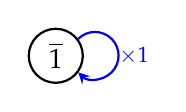
\begin{tikzpicture}[->,>=stealth,auto,node distance=3cm,
  thick,main node/.style={circle,draw}]

  \node[main node] (1) {$\overline{1}$};
\draw[blue]	(1.37) arc (135:-135:3mm) node[pos=0.3,below right] {\footnotesize$\times 1$} (1);
\end{tikzpicture}\]
\end{minipage}
\quad\!
\begin{minipage}{0.53\textwidth}
$\ell(1) = 1 \neq 7 - 1$, so $1$ is \emph{not} primitive. 
\end{minipage}

\vspace*{2em}

\begin{minipage}{0.15\textwidth}
\qquad $a = 2$ 
\end{minipage}
\begin{minipage}{0.25\textwidth}
\[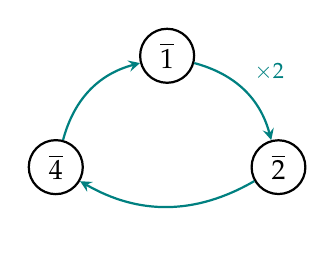
\begin{tikzpicture}[->,>=stealth,auto,node distance=2cm,
  thick,main node/.style={circle,draw}]

  \node[main node] (1) {$\overline{1}$};
  \node[main node] (2) [below right of= 1] {$\overline{2}$};
  \node[main node] (3) [below left of=1] {$\overline{4}$};
\path[every node/.style={font=\sffamily\small}]
	(1) edge[teal,bend left] node[] {\footnotesize$\times 2$} (2)
	(2) edge[teal,bend left] node[] {} (3)
	(3) edge[teal,bend left] node[] {} (1);
\end{tikzpicture}\]
\end{minipage}
\qquad
\begin{minipage}{0.53\textwidth}
$\ell(2) = 3 \neq 7 - 1$, so $2$ is \emph{not} primitive. 
\end{minipage}

\vspace*{2em}

\begin{minipage}{0.15\textwidth}
\qquad $a = 3$ 
\end{minipage}
\begin{minipage}{0.25\textwidth}
\[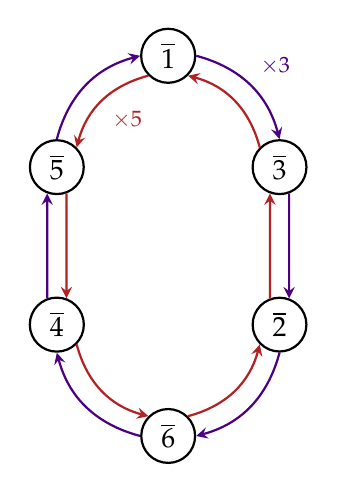
\begin{tikzpicture}[->,>=stealth,auto,node distance=2cm,
  thick,main node/.style={circle,draw}]

  \node[main node] (1) {$\overline{1}$};
  \node[main node] (2) [below right of=1] {$\overline{3}$};
  \node[main node] (3) [below of=2] {$\overline{2}$};
  \node[main node] (4) [below left of=3] {$\overline{6}$};
  \node[main node] (5) [above left of=4] {$\overline{4}$};
  \node[main node] (6) [above of=5] {$\overline{5}$};
\path[every node/.style={font=\sffamily\small}]
	(1.0) edge[indigo,bend left] node[] {\footnotesize$\times 3$} (2.90)
	(2.135) edge[firebrick,bend right] node[] {} (1.315)
	(2.290) edge[indigo] node[] {} (3.70)
	(3.110) edge[firebrick] node[] {} (2.250)
	(3.270) edge[indigo,bend left] node[] {} (4.0)
	(4.45) edge[firebrick,bend right] node[] {} (3.225)
    (4.180) edge[indigo,bend left] node[] {} (5.270)
    (5.315) edge[firebrick,bend right] node[] {} (4.135)
    (5.110) edge[indigo] node[] {} (6.250)
    (6.290) edge[firebrick] node[] {} (5.70)
    (6.90) edge[indigo,bend left] node[] {} (1.180)
    (1.225) edge[firebrick,bend right] node[] {\footnotesize$\times 5$} (6.45);
\end{tikzpicture}\]
\end{minipage}
\qquad
\begin{minipage}{0.53\textwidth}
$\ell(3) = 6 = 7 - 1$, so $3$ \emph{is primitive}.\\[0.5em]
So is $5$, as the multiplicative inverse of $3$ modulo $7$ in $\Phi(7)$. 
\end{minipage}

\newpage

Our goal is to prove
\begin{theorem*}[Gauss]
Let $p$ be a prime number, then there exist primitive roots in $\Phi(p)$, and there are precisely $\varphi(p-1)$-many of them.
\end{theorem*}
\emph{e.g.} For $p = 7,\ \varphi(7-1) = \varphi(6) = \varphi(2)\varphi(3) = 1\cdot 2 = 2$. The theorem tells us that there are $2$ primitive roots modulo $7$, they're necessarily $3$ and $5$, as seen in the example above.

\vspace*{2em}

{\bf Notation.} For $p$ a prime, we let $\ff_p \coloneqq \zz/p\zz = \set{\overline{0},\,\overline{1},\,\ldots,\,\overline{p-1}}$.\\[0.5em]
Furthermore, $\ff_p^\times \coloneqq (\zz/p\zz)\setminus\set{\overline{0}} = \set{\overline{1},\,\ldots,\,\overline{p-1}}$; note that that the set of representatives of this set is exactly $\Phi(p)$.

\vspace*{2em}

\begin{definition}
Let $p$ be a prime number, a polynomial modulo $p$ is an expression
\[f(T) = a_dT^d + \cdots + a_1T + a_0\]
where the coefficients $a_0,\ldots,a_d \in \ff_p$. The set of all polynomials modulo $p$ is denoted $\ff_p[T]$.\\
\\
The \emph{degree} of $f(T)$, denoted $\deg f$, is the largest $d$ such that $a_d \neq \overline{0}$ in $\ff_p$.\\
\\
\textsl{Convention:} $\deg 0 \coloneqq -1$, where $0$ is the zero polynomial.
\end{definition}

\vspace*{1em}

We can add, subtract and multiply polynomials modulo $p$; that is, $\ff_p[T]$ is a ring.\\[0.5em]
\emph{e.g.} $p = 5$
\begin{align*}
f(T) &= \overline{4}T + \overline{2} & g(T) &= \overline{3}T^2 + \overline{2}T\\[0.5em]
\deg f &= 1 & \deg g &= 2
\end{align*}
\begin{align*}
f(T)g(T) &= (\overline{4}T + \overline{2})(\overline{3}T^2 + \overline{2}T)\\[0.5em]
&= \overline{12}T^3 + \overline{6}T^2 + \overline{8}T^2 + \overline{4}T\\[0.5em]
&= \overline{12}T^3 + \overline{14}T^2 + \overline{4}T\\[0.5em]
&= \overline{2}T^3 + \overline{4}T^2 + \overline{4}T = \overline{2}T^3 - T^2 - T,\quad \text{reducing$\modar{5}$}
\end{align*}

\vspace*{1em}

\begin{theorem}\label{degsumprod}
Let $p$ be a prime and $f(T),\,g(T) \in \ff_p[T]$ are non-zero. Then
\[\deg (fg) = \deg f + \deg g\]
\end{theorem}
\begin{proof}
Let $d = \deg f$ and $e = \deg g$, then
\begin{align*}
f(T) &= a_dT^d + (\text{terms}),\quad a_d \neq \overline{0}\\[0.5em]
g(T) &= b_eT^e + (\text{terms}),\quad b_e \neq \overline{0}
\end{align*}
Then $f(T)g(T) = a_db_e T^{d+e} + (\text{terms})$. Since $a_d,b_e \neq \overline{0}$ in $\ff_p$, where $p$ is prime, necessarily $a_db_e \neq \overline{0}$. Therefore $\deg(fg) = d + e = \deg f + \deg g$. 
\end{proof}

%\vspace*{1em}

\begin{remark}
If $m$ was composite, then we can similarly consider polynomials modulo $m$ and we can add, subtract and multiply such polynomials. But the previous theorem does not hold.\\[0.5em]
For example, let $m = 6$, and consider the following polynomials modulo $6$
\[f(T) = \overline{3}T + \overline{2},\qquad g(T) = \overline{2}T^3\]
So, \[f(T)g(T) = \overline{4}T^3 + \overline{6}T^4 = \overline{4}T^3 + \overline{0}T^4 = \overline{4}T^3.\] Then $\deg (fg) = 3 \neq 4 = \deg f + \deg g$.
\end{remark}

\vspace*{0.5in}

\subsection{Problems}
\vspace{0.1in}

\begin{problem}\label{Problem 12.1}
Let $f(n)$ and $g(n)$ be two complex-valued functions of positive integers $n > 0$. Recall the definition of convolution
\[(f * g)(n) = \sum_{d\in \mathscr{D}(n)}f(d)g\left(\frac{n}{d}\right) = \sum_{\substack{ab = n\\ a,b>0}}f(a)g(b).\]
\begin{itemize}
\item[(a)] Prove that the two functions $f * g$ and $g * f$ are one and the same.\\
{\footnotesize (In other words: the convolution product is commutative.)}
\item[(b)] Let $\epsilon(n)$ be the function defined by the rule
\[\epsilon(n) = \begin{cases} 1 & \text{if $n = 1$}\\[0.5em] 0 & \text{if $n > 1$} \end{cases}.\]
Prove that $f = \epsilon * f$. Combined with (a), this tell us $f*\epsilon = f = \epsilon * f$.\\
{\footnotesize (In other words: $\epsilon$ acts as the neutral element for the convolution.)}
\item[(c)] Let $h:\zz_+ \to \cc$ be a third function. Prove that
\[(f * g) * h = f * (g * h).\]
{\footnotesize (In other words, the convolution product is associative.)}
\item[(d)] Suppose that $f(1) \neq 0$. Define the function $i_f(n)$ by induction on the divisibility of $n$ as follows. First define
\begin{equation}\label{12eq1}
i_f (1) \coloneqq \frac{1}{f(1)}. \tag{12.1.d.1}
\end{equation}
Given an integer $n > 1$, assume we have defined $i_f(d)$ for all the proper positive divisors $d$ of $n$, this is the set $\mathscr{D}_{\text{pr}}(n) \coloneqq \mathscr{D}(n)\setminus\set{n}$. Then proceed to define
\begin{equation}\label{12eq2}
i_f (n) \coloneqq -\frac{1}{f(1)} \sum_{d\in \mathscr{D}_{\text{pr}}(n)}i_f(d)f\left(\frac{n}{d}\right). \tag{12.1.d.2}
\end{equation}
Compute $i_f(n)$ for $n = 2,\, 3,\, 4,\, 5,\, 6$ in the particular case where $f$ is the identity function: $f(n) = n$.
\item[(e)] Return to the general case where $f(n)$ is any function such that $f(1) \neq 0$, and $i_f$ is defined by the formulae \eqref{12eq1} and \eqref{12eq2}.\\[0.5em]
Prove that $i_f * f = \epsilon$.\\[0.5em]
Prove that if $j(n)$ is any other complex valued function such that $j * f = \epsilon$, then we necessarily have $j = i_f$.\\[0.2em]
{\footnotesize Hint: look back to our proof of ``uniqueness" of multiplicative inverses modulo $m$.}
\end{itemize}
\end{problem}

\vspace*{0.1in}

\begin{problem}[M{\"o}bius Inversion]\label{Problem 12.2} Let $f$ and $g$ be two arithmetic functions, that is $f,g: \zz_+ \to \cc$. Prove that
\[g(n) = \sum_{d\in \mathscr{D}(n)}f(d)\quad \text{if and only if}\quad f(n) = \sum_{d\in \mathscr{D}(n)}\mu(d)g\left(\frac{n}{d}\right)\]
In the language of convolution, the question is asking you to prove that
\[g = f * \one \quad \text{if and only if}\quad f = g * \mu\]
This is sometimes called the M{\"o}bius Inversion formula. You can now probably see that Lemma \ref{totientsum} was just an application of this.\\
\\
Consider the arithmetic function defined as $p_k(n) = n^k$; in particular, $p_0 = \one$ and $p_1 = \id$. Using M{\"o}bius Inversion, prove that
\[p_k = \sigma_k * \mu.\]
\end{problem}

\vspace*{0.1in}

\begin{problem}\label{Problem 12.3}\hfill
\begin{itemize}
\item[(a)] Compute $\ell(a)$ in the $3 \times 4$ cases: $a = 2, 3, 6$ and $p = 7, 11, 13, 17$.
\item[(b)] For the primes $p = 7, 11, 13, 17$, list all the primitive roots modulo $p$.
\end{itemize}
\end{problem}
\newpage

\section{Lecture 13 (11/4)}
\vspace*{1em}

\begin{definition}
An element $a$ of $\ff_p$ is a \emph{root} of $f(T) \in \ff_p[T]$, if $f(a) = \overline{0}$.\\[0.5em]
Say an integer $x$ is a root of a polynomial modulo $p$ if $\overline{x}$ is.
\end{definition}
\vspace*{0.5em}
\emph{e.g.} Consider $p = 5,\ g(T) = \overline{3}T^2 + \overline{2}T$
\begin{itemize}
\item $a = \overline{0}$ is a root of $g(T)$, since $g(\overline{0}) = \overline{0}$.
\item $a = \overline{1}$ is a root of $g(T)$, since $g(\overline{1}) = \overline{3}\cdot \overline{1}^2 + \overline{2}\cdot\overline{1} = \overline{5} = \overline{0}$.
\item $a = \overline{2}$ is \emph{not} a root of $g(T)$, since $g(\overline{2}) = \overline{3}\cdot \overline{2}^2 + \overline{2}\cdot\overline{2} = \overline{16} = \overline{1} \neq \overline{0}$.
\end{itemize}

\vspace*{1em}

\begin{proposition}\label{primlin}
Consider a linear polynomial $f(T) = aT + b \in \ff_p[T]$, in particular $a \neq \overline{0}$ in $\ff_p$. Then $f(T)$ has a unique root in $\ff_p$.
\end{proposition}
\begin{proof}
Since $a \neq \overline{0}$, there exists a unique $c \in \ff_p$ such that $ac = 1$, by Corollary \ref{primeinv}. Now, let $x \in \zz$, then $x$ is a root of $f(T)$ if and only if $f(\overline{x}) = a\overline{x} + b = 0$ if and only if $a\overline{x} = -b$ if and only if $\overline{x} = -cb$. 
\end{proof}

\vspace*{2em}

The set of polynomials modulo $p,\ \ff_p[T]$, behaves a lot like $\zz$.
\begin{theorem}[Division algorithm in polynomials modulo $p$]\label{divalgfact}
Let $p$ be a prime, and $f(T),\,g(T) \in \ff_p[T]$. Assume that $g(T)$ is not the zero polynomial ($\deg g\geq 0$). Then there exist polynomials modulo $p,\ q(T)$ and $r(T)$, such that
\[f(T) = g(T)q(T) + r(T),\quad \deg r < \deg g\]
\end{theorem}

\vspace*{1em}

\emph{e.g.} Consider $p = 5$ and polynomials $f(T) = T^3 + \overline{4}T + \overline{2},\ g(T) = T^2 + T + \overline{2}$
\[
\arraycolsep=1pt
\renewcommand\arraystretch{1.2}
\begin{array}{*1r @{\hskip\arraycolsep}c@{\hskip\arraycolsep} *{11}r}
        &          & T & - & \overline{1}{\color{white}T^1} &  &  &  &\\
\cline{2-9}
T^2 + T + \overline{2} & \longdiv & T^3 & + & \overline{0}T^2 & + & \overline{4}T & + & \overline{2}\\
        &         & T^3 & + & T^2 & + & \overline{2}T&&&&&\quad & \text{(subtract)}\\
\cline{3-7}
        &          &   & - & T^2 & + & \overline{2}T & + & \overline{2} \\
        &          &   & - & T^2 & - & T & - & \overline{2} &&&\quad & \text{(subtract)}\\
\cline{4-9}
        &          &   &   &   &   & \overline{3}T & + &  \overline{4}
\end{array}
\]
Therefore 
\[f(T) = \underbrace{(T-\overline{1})}_{q(T)}g(T) + \underbrace{(\overline{3}T + \overline{4})}_{r(T)}\]

\vspace*{0.5em}

\begin{definition}
Let $p$ be a prime number, and polynomial below means polynomial modulo $p$
\begin{itemize}
\item A \emph{unit polynomial} is a non-zero constant polynomial, that is a polynomial of degree $0$.
\item A polynomial $f(T)$ is an \emph{irreducible polynomial} if
\begin{itemize}
\item[(IR1)] $\deg f \geq 1$ (non-constant, equivalently non-unit); and\label{IR1}
\item[(IR2)] If $g(T)$ and $h(T)$ are polynomials such that \label{IR2}
\[f(T) = g(T)h(T)\]
then either $g(T)$ is a unit polynomial, or $h(T)$ is.
\end{itemize}
\end{itemize}
\end{definition}

\vspace*{2em}

Here, we have an analogy with $\zz$
\begin{align*}
\text{unit polynomials} &\longleftrightarrow \pm 1 \text{ in } \zz\\[0.5em]
\text{irreducible polynomials} &\longleftrightarrow \text{prime numbers in } \zz\\[0.5em]
\end{align*}

%\vspace*{1em}

\begin{example}
For any $a \in \ff_p$, the linear polynomial $f(T) = T - a \in \ff_p[T]$ is irreducible.
\end{example}
\begin{proof}[Answer]
Clearly (IR1) of Definition \ref{IR1} is met. Let's prove (IR2); suppose
\[T - a = g(T)h(T),\]
then $1 = \deg (T - a) = \deg g + \deg h$. Therefore, $\deg g = 0$ and $\deg h = 1$, or vice versa (since $f \neq 0$). Hence $g(T)$ is a unit, or $h(T)$ is. Thus, $f(T)$ is irreducible.
\end{proof}

\vspace*{1em}

In fact, there are infinitely many polynomials modulo $p$. One proves this similarly as one proves the infinitude of primes once one has Theorem \ref{polyfact}.

\vspace*{2em}

\begin{definition}
Let $p$ be a prime and $f(T) \in \ff_p[T]$. Let $d = \deg f$, and write
\[f(T) = a_d T^d + \cdots + a_1 T + a_0\]
Then $a_d$ is called the \emph{leading coefficient of $f(T)$}. If $a_d = \overline{1}$, call $f(T)$ a \emph{monic polynomial}.\\
\\
Any non-zero polynomial $f(T)$ with leading coefficient $a_d$ can be uniquely written as 
\[f(T) = a_d\cdot (\text{monic polynomial})\]
\end{definition}

\vspace*{1em}

\begin{theorem}[Unique factorisation in polynomials modulo $p$]\label{polyfact}
Let $f(T)$ be a non-zero polynomials modulo $p$, where $p$ is prime. Then $f(T)$ can be uniquely written as
\[f(T) = c\cdot p_1(T)^{e_1}p_2(T)^{e_2}\cdots p_r(T)^{e_r}\]
where
\begin{itemize}
\item $c$ is the leading coefficient of $f(T)$;
\item $p_1(T),\,p_2(T),\ldots,\,p_r(T)$ are monic irreducible polynomials modulo $p$; and 
\item $e_1,\ldots,e_r>0$ are integers.
\end{itemize}
\end{theorem}
\begin{proof}
The proof is similar to the proof of uniqueness of prime factorisation in $\zz$, Theorem \ref{fundarith}. One applies (strong) induction on $\deg f$.
\end{proof}

\vspace*{1.5em}

\begin{lemma}\label{factthm}
Let $p$ be prime, and $f(T) \in \ff_p[T]$ with $x \in \zz$. Then $x$ is a root of $f(T)$ if and only if $T - \overline{x}$ divides $f(T)$.
\end{lemma}
\begin{proof}
We apply the division algorithm to $f(T)$ and $T - \overline{x}$,
\[f(T) = (T-\overline{x})q(T) + r(T),\]
where $q(T),r(T) \in \ff_p[T]$ and $\deg r < \deg (T - \overline{x}) = 1$. Therefore $\deg r = 0$ or $-1$, i.e., $r(T)$ is a unit (a constant polynomial) or the zero polynomial. Say, $r = r(T) \in \ff_p$; so we have
\[f(T) = (T-\overline{x})q(T) + r\]
Evaluating the above equation at $\overline{x}$ gives us 
\[f(\overline{x}) = (\overline{x}-\overline{x})q(\overline{x}) + r = r.\]
Hence, $f(T)$ has $x$ as a root if and only if $f(\overline{x}) = 0$ if and only if $r = 0$. Thus, $f(T)$ has $\overline{x}$ as a root if and only if $f(T) = (T-\overline{x})q(T)$ if and only if $T - \overline{x}$ divides $f(T)$.
\end{proof}

\vspace*{1.5em}

\begin{theorem}
Let $p$ be a prime number and $f(T) \in \ff_p[T]$. Assume that $f(T)$ is non-zero, then \[\card\set{\text{distinct roots of $f(T)$}} \leq \deg f.\]
\end{theorem}
\begin{proof}
We will induct on $\deg f$. If $\deg f = 1$, then $f(T) = aT + b$ with $a \neq \overline{0}$. Then, by Proposition \ref{primlin}, $f$ has a unique root in $\ff_p$. Hence, the base case holds.\\[0.5em]
Assume the induction hypothesis. Suppose $f(T)$ has no roots in $\ff_p$, then nothing to prove and the result holds (since $0 \leq \deg f$).\\[0.5em]
Therefore, assume $f$ has a root, say $a \in \ff_p$. Then, by Lemma \ref{factthm}, we have $f(T) = (T - a)g(T)$, for some polynomial $g(T) \in \ff_p[T]$. So, $\deg g = \deg f - 1$, by Theorem \ref{degsumprod}.\\[0.5em]
Therefore, by the induction hypothesis, $g(T)$ has at most $(\deg g)$-many distinct roots. Note that 
\begin{align*}
\set{\text{roots of $f(T)$}} &= \set{a} \cup \set{\text{roots of $g(T)$}}
\end{align*}
Hence,\\[-2em]
\begin{align*}
\card\set{\text{roots of $f(T)$}} &\leq \card\set{a} + \card\set{\text{roots of $g(T)$}}\\[0.5em]
&\leq 1 + \deg g\\[0.5em]
&= 1 + (\deg f - 1)\\[0.5em]
&= \deg f
\end{align*}
%\[\]
%Hence, 
%\begin{align*}
%\card\set{\text{roots of $f(T)$}} &\leq \card\set{a} + \card\set{\text{roots of $g(T)$}}\\[0.5em]
%&\leq 1 + \deg g = 1 + (\deg f - 1) = \deg f
%\end{align*}
Thus, the result holds, by the principle of mathematical induction.
\end{proof}

%\vspace*{1em}

\begin{remark}
As in a similar case before, the assumption that $p$ is prime is important. If $m$ was composite, then we can similarly consider polynomials modulo $m$ and define the notion of degree and roots of such polynomials. But unlike in the case of primes, the number of roots of these polynomials are then not bounded by degree.\\[0.5em]
For example, let $m = 8$, and consider polynomial $f(T) = T^2 - \overline{1}$ modulo $8$. Note that
\begin{align*}
f(\overline{1}) &= \overline{1}^2 - \overline{1} = \overline{0}\\[0.5em]
f(\overline{3}) &= \overline{3}^2 - \overline{1} = \overline{8} = \overline{0}\\[0.5em]
f(\overline{5}) &= \overline{5}^2 - \overline{1} = \overline{24} = \overline{0}\\[0.5em]
f(\overline{7}) &= \overline{7}^2 - \overline{1} = \overline{48} = \overline{0}
\end{align*}
Clearly $\overline{1},\,\overline{3},\,\overline{5}$ and $\overline{7}$ are distinct elements in $\zz/8\zz$. Therefore, we have found at least $4$ roots of a degree $2$ polynomial. 
\end{remark}

\vspace*{0.5in}

\subsection{Problems}
\vspace{0.1in}

\begin{problem}\label{Problem 13.1}\hfill
\begin{itemize}
\item[(a)] Let $f(T)$ be an irreducible polynomial modulo $p$, and consider any $a \in \ff_p$ such that $a \neq \overline{0}$. Prove that $g(T) \coloneqq af(T)$ is also irreducible.
\item[(b)] Let $f(T)$ be a polynomial modulo $p$, a prime, of degree $2$ or $3$. Prove that $f(T)$ is irreducible if and only if $f(T)$ has no roots modulo $p$.\\[0.2em]
{\footnotesize Hint: prove the contrapositive, look at the degrees of the factors of $f(T)$ and invoke a theorem from class.}
\\[0.5em]
Give an example illustrating why this reasoning does not help us determine if a given polynomial (modulo $p$) of degree $\geq 4$ is irreducible.
\end{itemize}
\end{problem}

\vspace*{0.1in}

\begin{problem}\label{Problem 13.2}
Let $p = 5$ and consider two polynomials mod $p$:
\begin{align*}
f(T) &= T^3 + \overline{3}T^2 + \overline{2}T + 1\\[0.5em]
g(T) &= \overline{2}T^4 + \overline{4}T^3 + T^2 + \overline{3}T + \overline{4}.
\end{align*}
\begin{itemize}
\item[(a)] Find the two polynomials mod $p$: $q(T)$ and $r(T)$, such that $\deg r < 3$ and
\[g(T) = f(T)q(T) + r(T).\]
\item[(b)] Apply the Division Algorithm to find the greatest common divisor of $f(T)$ and $g(T)$. Show your work. As in the case with integers, the $\gcd$ is the last non-zero remainder.
\item[(c)] Prove or disprove: The $\gcd$ that you have found in (b) is irreducible.\\[0.1em]
{\footnotesize Hint: use Problem \ref{Problem 13.1}.}
\item[(d)] Find the unique decompositions of $f(T)$ and $g(T)$ into irreducible polynomials mod $p$.
\end{itemize}
\end{problem}
\newpage

\section{Lecture 14 (11/9)}
\vspace*{1em}

\begin{example}
Consider the polynomial $f(T) = T^3 + \overline{2} \in \ff_5[T]$, let's find the unique factorisation into irreducibles of $f$.
\end{example}
\begin{proof}[Answer]
First, we check if $f(T)$ has a root modulo $5$; note
\begin{center}
{\renewcommand{\arraystretch}{1.5}%
\begin{tabular}{|c|c|c|c|c|c|}
  \hline
  $a$ & $\overline{0}$ & $\overline{1}$ & $\overline{2}$ & $\overline{3}$ & $\overline{4}$ \\
  \hline
  $f(a)$ & $\overline{2}$ & $\overline{1} + \overline{2} = \overline{3}$ & 
  $\overline{8} + \overline{2} = \overline{0}$ & $\overline{27} + \overline{2} = \overline{4}$ & $\overline{64} + \overline{2} = \overline{1}$ \\
  \hline
\end{tabular}}\\
\end{center}
Therefore $\overline{2}$ is a root of $f(T)$, hence by Corollary \ref{factthm} we have that $T - \overline{2}$ divides $f(T)$. Thus, 
\[f(T) = (T-\overline{2}) g(T),\]
for some polynomial $g(T) \in \ff_5[T]$ and $\deg g = 2$. We employ long division to compute $g(T)$
\[
\arraycolsep=1pt
\renewcommand\arraystretch{1.2}
\begin{array}{*1r @{\hskip\arraycolsep}c@{\hskip\arraycolsep} *{11}r}
        &          & T^2 & + & \overline{2}T & + & \overline{4} &  &\\
\cline{2-9}
T - \overline{2} & \longdiv & T^3 & + & \overline{0}T^2 & + & \overline{0}T & + & \overline{2}\\
        &         & T^3 & - & \overline{2}T^2 &  & &&&&&& \text{(subtract)}\\
\cline{3-5}
        &          &   &  & \overline{2}T^2 & + & \overline{0}T & + & \overline{2} \\
        &          &   &  & \overline{2}T^2 & - & \overline{4}T &  &  &&&& \text{(subtract)}\\
\cline{5-7}
        &          &   &   &   &   & \overline{4}T & + & \overline{2} \\
        &          &   &  & & & \overline{4}T & - & \overline{8} &&&& \text{(subtract)}\\
\cline{7-9}
        &          &   &   &   &   & &  & \overline{10} &= \overline{0}&&
\end{array}
\]
Therefore $g(T) = T^2 + \overline{2}T + \overline{4}$, hence
\[f(T) = (T-\overline{2})(T^2 + \overline{2}T + \overline{4}) = (T+\overline{3}) (T^2 + \overline{2}T + \overline{4})\]
Note,
\begin{center}
{\renewcommand{\arraystretch}{1.5}%
\begin{tabular}{|c|c|c|c|c|c|}
  \hline
  $a$ & $\overline{0}$ & $\overline{1}$ & $\overline{2}$ & $\overline{3}$ & $\overline{4}$ \\
  \hline
  $g(a)$ & $\overline{4}$ & $\overline{7} = \overline{2}$ & $\overline{12} = \overline{2}$ & $\overline{19} = \overline{4}$ & $\overline{28} = \overline{3}$ \\
  \hline
\end{tabular}}\\
\end{center}
Thus, by Problem \ref{Problem 13.1}, $g(T)$ is irreducible since it has no roots modulo $5$. Therefore the factorisation that we obtained for $f(T)$ is its factorisation into irreducibles.
\end{proof}

\vspace*{1.5em}

\begin{definition}[Recall]
Let $p$ be a prime number and $a \in \Phi(p)$, then
\begin{itemize}[leftmargin=*]
\item[] $\begin{aligned}\bullet\quad \ell(a) &= \text{the common length of the cycles in the dynamics of \fbox{$\times a \modar{p}$} in $\Phi(p)$}\\[0.5em]  &= \text{the smallest positive integer $\ell$ such that $a^\ell \equiv 1 \modar{p}$} \end{aligned}$
\item[] $\begin{aligned}\bullet\quad c(a) &= \text{the number of cycles  in the dynamics of \fbox{$\times a \modar{p}$} in $\Phi(p)$}\end{aligned}$
\end{itemize}
In the course of proving Theorem \ref{euler-fermat}, we noted that $c(a)\cdot\ell(a) = \card\Phi(p) = \varphi(p) = p-1$.
\end{definition}

%\vspace*{1.5em}

\begin{lemma}
Let $p$ be a prime and $\lambda > 0$ be an integer; define
\[\Phi_\lambda(p) \coloneqq \setp{a \in \Phi(p)}{\ell(a) = \lambda}\]
Then, the set $\Phi_\lambda(p)$ has either $0$ (that is, the set is empty) or $\varphi(\lambda)$-many elements.
\end{lemma}
\begin{proof}
Suppose $\Phi_\lambda(p)$ is non-empty, we must prove that $\card\Phi_\lambda(p) = \varphi(\lambda)$. So, let $a \in \Phi_\lambda(p)$, in particular $\ell(a) = \lambda$.\\[0.5em]
Then, for $e = 0,\,1,\,\ldots,\,\lambda - 1$, we have
\[(a^e)^{\lambda} = (a^\lambda)^e \equiv 1^e \equiv 1 \modar{p}\]
Therefore, the polynomial $f(T) = T^\lambda - \overline{1} \in \ff_p[T]$ has $a^0,\,a^1,\,\ldots,\, a^{\lambda - 1}$ as roots. Moreover, since $\ell(a) = \lambda$, these are necessarily distinct modulo $p$.\\[0.5em]
Since $\deg f = \lambda$ and we found $\lambda$-many distinct roots of $f$, the set $R_a = \setp{a^e}{0 \leq e < \lambda}$ necessarily consists of all roots of $f$, and thus
\[T^\lambda - \overline{1} = (T - \overline{a}^0)(T - \overline{a}^1)\cdots(T - \overline{a}^{\lambda - 1})\]
Now, if $b \in \Phi_\lambda(p)$ was arbitrary, then by assumption $\ell(b) = \lambda$ and so $b^\lambda \equiv 1 \modar{p}$. Hence, $b$ is a root of $T^\lambda - \overline{1}$, and therefore, necessarily, $\overline{b} = \overline{a}^e$, for some $e = 0,\,1,\,\ldots,\,\lambda - 1$.\\
\\
Thus, to count $\Phi_\lambda(p)$, it suffices to focus on $a^e$. So, the question we want to ask is: what is $\ell(a^e)$? As this answer will tell us for what $e$ is $a^e \in \Phi_\lambda(p)$.\\
\\
If $k>0$ is an integer such that $(a^e)^k \equiv 1 \modar{p}$, then 
\[a^{ek} \equiv 1 \modar{p} \iff \ell(a) \mid ek \iff \lambda \mid ek \iff \frac{\lambda}{\gcd(e,\lambda)}\mid k\]
The only unjustified statement is the final statement, so let's prove that.\\
\begin{subproof}
Let $d = \gcd(e,\lambda)$.\\[1em]
($\Rightarrow$) By B\'ezout's Identity $d = ex + \lambda y$ for some integers $x,y$. Therefore $dk = ekx + \lambda ky$. Since $\lambda \mid ek$ and clearly $\lambda \mid \lambda k$, hence $\lambda \mid (ekx + \lambda ky) = dk$ and thus $(\lambda/d)\mid k$.\\[1em]
($\Leftarrow$) Since $d\mid e$, therefore $dk \mid ek$. By assumption $(\lambda/d) \mid k$, hence $\lambda \mid dk$. By transitivity of divisibility, we obtain $\lambda \mid ek$.
\end{subproof}
\vspace*{1em}
Therefore, since $\ell(a^e)$ is the minimum such $k$, necessarily $\ell(a^e) = \lambda/\gcd(e,\lambda)$.\\
\\
Hence, $\ell(a^e) = \lambda$ if and only if $\gcd(e,\lambda) = 1$. Thus,
\begin{align*}
\card\Phi_\lambda(p) &= \card\setp{a^e}{0 \leq e < \lambda\text{ and }\gcd(e,\lambda) = 1}\\[0.5em]
&= \card\setp{e}{0 \leq e < \lambda\text{ and }\gcd(e,\lambda) = 1}\\[0.5em]
&= \card\Phi(\lambda)\\[0.5em]
&= \varphi(\lambda)\\[-3em]
\end{align*}
\end{proof}

%\vspace*{1em}

\begin{theorem}[Gauss]\label{gaussprim}
Let $p$ be prime. Then there are exactly $\varphi(p-1)$-many primitive roots in $\Phi(p)$. Recall that primitive roots are those $a \in \Phi(p)$ such that $\ell(a) = p-1$.
\end{theorem}
\begin{proof}
Since $\ell(a)\cdot c(a) = p-1$, for any $a \in \Phi(p)$, we have $\ell(a) \mid (p-1)$. Furthermore, note that $\ell(a) > 0$; hence $\ell(a) \in \mathscr{D}(p-1)$ for any $a$.\\
\\
Now, for each $\lambda \in \mathscr{D}(p-1)$, the previous Lemma tells us that
\[\Phi_\lambda(p) = \setp{a \in \Phi(p)}{\ell(a) = \lambda}\]
has either $0$ or $\varphi(\lambda)$-many elements. Our aim is to prove that for any such $\lambda$, we always have $\Phi_\lambda(p) \neq \emptyset$, and then the result will follow by looking at $\lambda = p-1$, since $\Phi_{p-1}(p)$ is exactly the set of primitive roots.\\
\\
Note for $\lambda_1 \neq \lambda_2$, necessarily $\Phi_{\lambda_1}(p) \cap \Phi_{\lambda_2}(p) = \emptyset$. Therefore, $\displaystyle\Phi(p) = \coprod_{\lambda \in \mathscr{D}(p-1)}\Phi_{\lambda}(p)$. Hence,
\[p - 1 = \card\Phi(p) = \sum_{\lambda \in \mathscr{D}(p-1)}\card\Phi_\lambda(p) = \sum_{\lambda \in \mathscr{D}(p-1)}\begin{cases}0\quad\text{(or)}\\ \varphi(\lambda)\end{cases}\]
Now, by Lemma \ref{totientsum}, we also have that
\[\sum_{\lambda \in \mathscr{D}(p-1)}\varphi(\lambda) = p-1\]
Suppose, there existed a $\lambda_0 \in \mathscr{D}(p-1)$ such that $\Phi_{\lambda_0}(p) = \emptyset$, i.e. $\card\Phi_{\lambda_0}(p) = 0$. Then
\[\sum_{\lambda \in \mathscr{D}(p-1)}\varphi(\lambda) = p-1 = \card\Phi(p) = \sum_{\lambda \in \mathscr{D}(p-1)}\card\Phi_\lambda(p) = \sum_{\lambda \in \mathscr{D}(p-1) \setminus\set{\lambda_0}}\card\Phi_\lambda(p) < \sum_{\lambda \in \mathscr{D}(p-1)}\varphi(\lambda);\]
giving us a contradiction.\\
\\
Thus, $\Phi_\lambda(p) \neq \emptyset$, for all $\lambda \in \mathscr{D}(p-1)$. In particular, $\Phi_{p-1}(p) \neq \emptyset$, and therefore \[\card\Phi_{p-1}(p) = \varphi(p-1).\]
We have concluded more, not only did we prove that there exist primitive roots and there are $\varphi(p-1)$ of them, but also that there are numbers in $\Phi(p)$ that achieve every possible length $\lambda$ (necessarily a positive divisor of $p-1$) and that there are $\varphi(\lambda)$-many of them.
\end{proof}

\vspace*{2em}

{\bf An Application of Gauss' Theorem on Primitive Roots (Theorem \ref{gaussprim}).}\\[0.5em] Cryptography, \emph{public} key system. Diffie-Helman key exchange.
\[\begin{tikzcd}
	& {\text{Eve}} \\
	{\text{Alice}} & {} & {\text{Bob}}
	\arrow[squiggly, from=2-1, to=2-3]
	\arrow[bend left,dashed, from=1-2, to=2-2]
\end{tikzcd}\]
Alice wants to encrypt a message so that \emph{only} Bob can decrypt it, not Eve. 
\begin{itemize}
\item[(1)] Alice chooses a prime $p\ (\sim 2^{2000})$ such that $\varphi(p-1)$ also has a large prime factor, and finds a primitive root $g$ modulo $p$. Publishes $(p,g)$, the \emph{public key}.
\item[(2)] Alice chooses $a\modar{p-1}$ (\emph{private key}) and computes $A \coloneqq g^a \modar{p}$ and send it to Bob.\\[0.5em]
Bob chooses $b\modar{p-1}$ (\emph{private key}) and computes $B \coloneqq g^b \modar{p}$ and sends it to Alice.
\[\begin{tikzcd}
	{\text{Alice}} & {} & {\text{Bob}}
	\arrow[bend left,squiggly, from=1-1, to=1-3,"A"]
	\arrow[bend left,squiggly, from=1-3, to=1-1,"B"]
\end{tikzcd}\]
\item[(3)] Alice computes $B^a\modar{p}$ and Bob computes $A^b \modar{p}$, both are $\equiv g^{ab} \modar{p}$. This is their secret $S$.
\item[(4)] Eve knows $(g,p,A,B)$. Can Eve find out what $S$ is?\\[0.5em]
This is very hard (that is, takes a lot of time and computation power). If Eve knows $a$ or $b$, then the security has been broken. But finding $a$ from $A \equiv g^a \modar{p}$ is difficult. This is the \emph{discrete logarithm problem}.
\end{itemize}

\vspace*{0.5in}

\subsection{Problems}
\vspace{0.1in}

\begin{problem}\label{Problem 14.1}
Let $a \in \Phi(m)$ for a modulus $m$, and define $\ell(a)$ to be the smallest positive integer such that 
\[a^{\ell(a)} \equiv 1 \modar{m};\]
that is, $\ell(a)$ is the length of the cycles in the multiplicative modular dynamics given by \[\fbox{$\times a \modar{m}$}:\Phi(m) \to \Phi(m).\]
We have already seen that $\ell(a) \mid \varphi(m)$.
\begin{itemize}
\item[(a)] Prove that if $e$ is any integer such that $a^e \equiv 1 \modar{m}$, then $\ell(a) \mid e$.\\
{\footnotesize Hint: use the division algorithm with respect to $e$ and $\ell(a)$ arriving at a contradiction to the minimality of $\ell(a)$.}
\item[(b)] Suppose $p$ is an odd prime and $q$ is a prime factor of $2^p - 1$. Prove that $q \equiv 1 \modar{2p}$.
\end{itemize}
\end{problem}

\vspace*{0.1in}

\begin{problem}\label{Problem 14.2}
Find the smallest positive integer $a$ such that $2^a \equiv 11 \modar{p}$, for the two primes: $p = 23$ and $p = 37$.
\end{problem}

\vspace*{0.1in}

\begin{problem}\label{Problem 14.3}
Find Alice and Bob's secret number $S$, if $g = 3,\ p = 17,\ A = 8$ and $B = 7$.
\end{problem}
\newpage

\section{Lecture 15 (11/16)}
\vspace*{1em}

\begin{center}
{\Large Assembling the Modular World}
\end{center}

Back to the motivation of modular arithmetic
\begin{proof}[e.g.]\renewcommand{\qedsymbol}{}
\begin{itemize}
\item[(1)] $x^2 + y^2 = 83$; we saw that it has no integer solutions by looking$\modar{4}$.
\end{itemize}
\begin{itemize}[leftmargin=4.4em]
\item[(2)] $x^2 + y^2 = 3z^2$; we saw that it has only one rational solution $(0,0,0)$ by looking$\modar{3}$.
\end{itemize}
Each modulus only gives us partial information. In order to get a fuller picture, we want to assemble this information into one. In the horizontal direction we list all the primes, and in the vertical direction we list the prime powers.
\end{proof}
\vspace*{-1em}
\[\begin{tikzcd}
\vdots \arrow[d, no head]                  &[-2.5em] \color{teal}\modar{72} \arrow[ld, no head] \arrow[rdd, no head] &[-2.5em] \vdots \arrow[d, no head]                  & \vdots \arrow[d, no head]      &                                &        \\
\color{teal}\modar{2^3} \arrow[d, no head] &                                   & \modar{3^3} \arrow[d, no head]             & \modar{5^3} \arrow[d, no head] & \vdots \arrow[d, no head]      &        \\[0.5em]
\modar{2^2} \arrow[d, no head]             &                                   & \color{teal}\modar{3^2} \arrow[d, no head] & \modar{5^2} \arrow[d, no head] & \modar{7^2} \arrow[d, no head] &        \\[0.5em]
\modar{2} \arrow[rr, no head]              &                                   & \modar{3} \arrow[r, no head]               & \modar{5} \arrow[r, no head]   & \modar{7} \arrow[r, no head]   & \cdots
\end{tikzcd}\]
We understand, for example, a given expression$\modar{72}$ by understanding the expression $\!{\color{teal}\modar{2^3}}$ and $\!{\color{teal}\modar{3^2}}$.

\vspace*{1.5em}

\begin{proof}[Question (Ancient Puzzle)]\renewcommand{\qedsymbol}{}
There are an unknown number of oranges, fewer than $100$. 
\begin{align*}
\text{If I group them in $3$s,} & \text{ then $2$ oranges are left.}\\[0.2em]
\text{If I group them in $5$s,} & \text{ then $3$ oranges are left.}\\[0.2em]
\text{If I group them in $7$s,} & \text{ then $2$ oranges are left.}
\end{align*}
How many oranges are there in total?
\end{proof}

\begin{proof}[Translation of the Question]\renewcommand{\qedsymbol}{}
Suppose $N$ is an integer such that $0< N \leq 100$, and
\[N \equiv 2\modar{3},\quad N \equiv 3 \modar{5},\quad N \equiv 2 \modar{7}\]
What is $N$?
\end{proof}

\vspace*{1.5em}

{\bf Notation} (non-standard). Let $d,e$ be moduli and $a,b$ are integers. For any integer $x$, we write
\[x \equiv [a,b]\modar{[d,e]},\quad \text{if }\ x \equiv a \modar{d}\ \text{ and }\ x \equiv b \modar{e}\]\\[0.2em]
\emph{e.g.} Let $d = 3,\,e = 5$, then $67 \equiv [1,2]\modar{[3,5]}$

%\vspace*{1em}

\begin{theorem}[Chinese Remainder Theorem, CRT]\label{crt}
Let $d$ and $e$ be moduli. Assume that $d$ and $e$ are coprime, that is $\gcd(d,e) = 1$. Then there's a one-to-one correspondence
\[\begin{tikzcd}
\set{(a,b) \in \zz^2\ \Bigg\vert \begin{minipage}{0.16\textwidth}
\begin{center}
$0 \leq a \leq d-1$\\[0.2em] $0 \leq b \leq e-1$
\end{center}
\end{minipage}\!\!}
 \arrow[r,leftrightarrow] &[1em] \setp{N \in \zz}{0\leq N \leq de-1}
\end{tikzcd}\]
in which solutions to $x \equiv [a,b]\modar{[d,e]}$ correspond to $y \equiv N\modar{de}$.
\end{theorem}

\vspace*{0.5em}

\emph{e.g.} We want to assemble the congruences
\[N \equiv [6,2]\modar{[7,5]}\]
\begin{itemize}[leftmargin=2em]
\item[(1)] Write each of the two congruences into integer equations
\begin{align*}
N \equiv 6\modar{7},\quad &\text{ if and only if}\quad N = 6 + 7x \text{,\ for some integer $x$}\\[0.5em]
N \equiv 2\modar{5},\quad &\text{ if and only if}\quad N = 2 + 5y \text{,\ for some integer $y$}
\end{align*}
\item[(2)] Combine the two equations into one.
\[6 + 7x = N = 2 + 5y\]
\[7x - 5y = -4\]
\item[(3)] Find \emph{one} particular solution using the division algorithm
\begin{align*}
7 &= 5\cdot 1 + 2 & 1 &= 5 - 2\cdot 2\\[0.5em]
5 &= 2\cdot 2 + 1 & &= 5 - 2(7-5)\\[0.5em]
2 &= 1\cdot 2 + 0 & &= 7(-2) + 5(3)
\end{align*}
So, we have
\[-4 = -4\cdot 1 = -4(7(-2) + 5(3)) = 7(8) - 5(12).\]
Therefore $(x,y) = (8,12)$.
\item[(4)] Return to $N$. Our computations give us
\[N = 7(8) + 6 = 62\]
is a solution to $N \equiv [6,2]\modar{[7,5]}$.
\end{itemize}
The Chinese Remainder Theorem tells us that $N = 62$ is unique upto$\modar{7\cdot 5}$. That is, if $M$ is another solution to $N \equiv [6,2]\modar{[7,5]}$, then $M \equiv 62\modar{35} \equiv 27\modar{35}$.

\vspace*{1.5em}

\begin{proof}[Proof of Theorem \ref{crt} (CRT)] 
Let's start by defining the sets under consideration
\begin{align*}
C_d &= \setp{a\in\zz}{0\leq a \leq d-1}\\[0.5em]
R_e &= \setp{b\in \zz}{0\leq b \leq e-1}\\[0.5em]
P_{de} &= \setp{N\in \zz}{0\leq N \leq de-1}
\end{align*}
and consider the function defined as
\[f:P_{de} \to C_d \times R_e,\ \ N \mapsto (a_N,b_N),\]
where
\begin{align*}
a_N &\coloneqq \text{natural representative of $N$ modulo $d$, i.e., the remainder in division of $N$ by $d$;}\\[0.2em]
b_N &\coloneqq  \text{natural representative of $N$ modulo $e$, i.e., the remainder in division of $N$ by $e$.}
\end{align*}
In particular, $a_N \equiv N \modar{d}$ and $b_N \equiv N \modar{e}$.\\
\\
\emph{Injectivity of $f$.} Say $M, N$ are such that they get mapped to the same element under $f$, say $(a,b)$. Then
\begin{align*}
M &\equiv [a,b]\modar{[d,e]}\\[0.2em]
N &\equiv [a,b]\modar{[d,e]}\\[0.2em]
\text{So, }\ M-N&\equiv [0,0]\modar{[d,e]}
\end{align*}
That is, $d\mid (M-N)$ and $e\mid (M-N)$. Since $d$ and $e$ are coprime, we have
\[de \mid (M-N)\]
Hence, $M - N = 0$ or $|M-N| \geq de$. Now, since $M,N \in P_{de}$, we have $0 \leq M,N \leq de-1$ since $M,N \in P_{de}$, this gives us
\[-(de - 1) \leq M-N \leq (de - 1).\]
That is, $|M - N| \leq de - 1 < de$. Thus, necessarily, $M - N = 0$. Therefore $f$ is injective.\\
\\
\emph{Bijectivity of $f$.} Note that $|P_{de}| = de$ and $|C_d \times R_e| = |C_d|\cdot |R_e| = de$. That is, $f$ is an injective map between two sets of the same size. Therefore, $f$ is a bijection. 
\end{proof}

\vspace*{1.5em}

\begin{remark}\label{crtprac}
The interpretation that we will use in practice is the following:\\[0.5em]
Given moduli $d$ and $e$ such that $\gcd(d,e) = 1$, then
\[x \equiv N \modar{de}\quad \text{if and only if}\quad x \equiv [N,N]\modar{[d,e]}\]
\end{remark}

\vspace*{1em}

\begin{remark}
One can use Theorem \ref{crt} to give another proof of the formula of the Euler totient function. One can, first, directly show that $\varphi(p^e) = p^{e-1}(p-1)$. Then, one shows that the one-to-one correspondence $f$ in Theorem \ref{crt} restricts to a one-to-one correspondence
\[\Phi(de) \to \Phi(d) \times \Phi(e)\]
Taking cardinalities, we obtain $\varphi(de) = \varphi(d)\varphi(e)$, whenever $\gcd(d,e)=1$. This shows that $\varphi$ is multiplicative.\\[1em]
Combining these two facts gives us the formula seen in Theorem \ref{totientform}.\\
\\
The real reason for all of this works is because the bijection $f$ in Theorem \ref{crt}, when $\gcd(d,e)=1$, was in fact a \emph{ring isomorphism} given as
\begin{align*}
f: \zz/de\zz &\to \zz/d\zz \times \zz/e\zz;\\[0.2em]
N\modar{de}&\mapsto (N\modar{d},N\modar{e})
\end{align*}
%Ring isomorphisms restrict to isomorphisms of the unit groups, i.e., $f$ restricts to the isomorphism
%\[(\zz/de\zz)^\times \to (\zz/d\zz)^\times \times (\zz/e\zz)^\times\]
\end{remark}

%\vspace*{2em}

{\bf Applications of the Chinese Remainder Theorem.}
\begin{itemize}[leftmargin=2em, itemsep=1.5em]
\item[I.] \emph{More then two congruences.} Recall the ancient riddle: find the positive integer $N \leq 100$ such that
\begin{align}
N &\equiv 2\modar{3}\label{arc1}\\
N &\equiv 2 \modar{7}\label{arc2}\\
N &\equiv 3 \modar{5}\label{arc3}
\end{align}
\textsl{Solution.} From \refp{arc1} and \refp{arc2}, we get that $N-2$ is divisible by $3$ and $7$. Since $3$ and $7$ are coprime, it follows that $N-2$ is divisible by $7\cdot 3 = 21$. Hence, \refp{arc1} and \refp{arc2} give us
\begin{align}
N &\equiv 2 \modar{21}\label{arc4}
\end{align}
We solve the simultaneous congruence given by \refp{arc3} and \refp{arc4}. We rewrite them as
\[N = 3 + 5x,\quad N = 2 + 21y\]
for some integers $x,y$. Therefore $3 + 5x = N = 2 + 21y$, giving us
\[5x - 21y = -1\]
An immediate solution is given by $(x,y) = (4,1)$ (alternatively, use the division algorithm). This gives us
\[N = 2 + 21(1) = 3 + 5(4) = 23\]
Now, the Chinese Remainder Theorem tells us that $N \equiv 23\modar{5\cdot 21}\equiv 23\modar{105}$ is the only solution modulo $105$. That is, the set of all positive solutions is $\setp{23 + 105k}{k \in \zz,\,k \geq 0}$. Since we were looking for $N\leq 100$, the answer is $N = 23$.

\item[II.] \emph{Quadratic Congruences.}
\begin{itemize}[leftmargin=*,itemsep=1.5em]
\item[IIa.] Find all integers $0 \leq x \leq 34$ such that
\[x^2 \equiv 29\modar{35}\]
One method: compute $0^2,\,1^2,\,2^2,\ldots,\,34^2\modar{35}$ and see if any one of them is $\equiv 29\modar{35}$.\\
\\
A better method: break $x^2 \equiv 29\modar{35}$ into two congruences;
\begin{align*}[left=\empheqlbrace]
x^2 \equiv 29\modar{5} &\equiv 4\modar{5}\label{qc1}\tag{$\underline{5}$}\\[0.1em]
x^2 \equiv 29\modar{7} &\equiv 1\modar{7}\label{qc2}\tag{$\underline{7}$}
\end{align*}
Since $5$ and $7$ are primes, we can use polynomial methods, i.e.
\begin{align*}
\refp{qc1} \iff x^2 - \overline{4} = 0 &\iff (x-\overline{2})(x+\overline{2}) = \overline{0}\\[0.5em]
&\iff x = \overline{2}\ \text{ or }\ x = -\overline{2} = \overline{3}\\[0.5em]
&\iff x \equiv 2\modar{5}\ \text{ or }\ x \equiv -2\modar{5}\\[1em]
\refp{qc2} \iff x^2 - \overline{1} = 0 &\iff (x-\overline{1})(x+\overline{1}) = \overline{0}\\[0.5em]
&\iff x = \overline{1}\ \text{ or }\ x = -\overline{1} = \overline{6}\\[0.5em]
&\iff x \equiv 1\modar{7}\ \text{ or }\ x \equiv -1\modar{7}
\end{align*}
Therefore, we have four possibilities
\begin{center}
\begin{tabular}{|c|c|c|}
\hline
&$x\equiv 1\modar{7}$&$x\equiv 6\modar{7}$\\
\hline
$x\equiv 2\modar{5}$ & $\bullet_1$& $\bullet_2$\\
\hline
$x\equiv 3\modar{5}$ & $\bullet_3$ & $\bullet_4$\\
\hline
\end{tabular}
\end{center}
\vspace*{0.2em}
\emph{e.g.} Let's consider $\bullet_1$, that is $x\equiv 1\modar{7}$ and $x\equiv 2\modar{5}$. Rewrite as
\[x = 1 + 7a \quad \text{and} \quad x = 2 + 5b\]
for some integer $a,b$. Then
\[7a - 5b = 1\]
An immediate solution is $(a,b) = (3,4)$ (alternatively, use the division algorithm). This tells us, $x = 1 + 7(3) = 22$. Hence the solution is $x \equiv 22\modar{35}$.\\
\\
Similar computations help us populate the table above, and we get our answer
\begin{center}
\begin{tabular}{|c|c|c|}
\hline
&$x\equiv 1\modar{7}$&$x\equiv 6\modar{7}$\\
\hline
$x\equiv 2\modar{5}$ & $x \equiv 22\modar{35}$& $x \equiv 27\modar{35}$\\
\hline
$x\equiv 3\modar{5}$ & $x \equiv 8\modar{35}$ & $x \equiv 13\modar{35}$\\
\hline
\end{tabular}
\end{center}
\vspace*{0.2em}
That is, $x = 8,\,13,\,22,\,27$ are the positive integers less than $35$ whose square is $\equiv 29\modar{35}$.
\item[IIb.] Find all integers $0 \leq x \leq 34$ such that
\[x^2 \equiv 6\modar{35}\]
Yes, we have a solution
\begin{align*}
\underset{\text{CRT}}{\iff}& \begin{cases} x^2 \equiv 6\modar{5}\\[0.2em] x^2\equiv 6\modar{7}\end{cases}\\[1.5em]
\iff& \begin{cases} x^2 \equiv 1\modar{5}\\[0.2em] x^2\equiv 6\modar{7}\end{cases}\\[1.5em]
\iff& \begin{cases} x \equiv 1\modar{5}\ \text{ or }\ x \equiv -1\modar{5}\\[0.2em] \text{\emph{never happens}}\end{cases}
\end{align*}
Since, note that
\begin{center}
\begin{tabular}{|c|c|}
\hline
$x\modar{7}$&$x^2\modar{7}$\\
\hline
$0$ & $0$\\
\hline
$1$ & $1$\\
\hline
$2$ & $4$\\
\hline
$3$ & $2$\\
\hline
$4$ & $2$\\
\hline
$5$ & $4$\\
\hline
$6$ & $1$\\
\hline
\end{tabular}
\end{center}
Conclusion: for no positive integer $x$ do we have have $x^2 \equiv 6\modar{35}$.
\end{itemize}
\end{itemize}

%\vspace*{2em}

\begin{center}
{\Large Quadratic Residues}
\end{center}

\begin{definition}
Let $p$ be a prime and let $n$ be an integer.
\begin{itemize}
\item Say $n$ (or $\overline{n}$) is a \emph{quadratic residue} (QR) modulo $p$ if $n\equiv x^2\modar{p}$ for some integer $x$.
%That is, there's a root modulo $p$ of the polynomial $T^2 - \overline{n} \in \ff_p[T]$.
\item Otherwise $n$ (or $\overline{n}$) is called a \emph{quadratic non-residue} (QNR).
\end{itemize}
We can rephrase this in terms of polynomials: $n$ is a QR if and only if $T^2 - \overline{n} \in \ff_p[T]$ is reducible. Therefore, one can interpret this as a method to test for irreducibilities of quadratic polynomials modulo $p$.
\end{definition}
\emph{e.g.} Let $p = 11$,
%\begin{center}
%{\renewcommand{\arraystretch}{1.5}%
%\begin{tabular}{|c|c|}
%\hline
%$x\modar{11}$&$x^2\modar{11}$\\
%\hline
%$\overline{0}$ & $\overline{0}$\\
%\hline
%$\overline{1}$ & $\overline{1}$\\
%\hline
%$\overline{2}$ & $\overline{4}$\\
%\hline
%$\overline{3}$ & $\overline{9}$\\
%\hline
%$\overline{4}$ & $\overline{16} = \overline{5}$\\
%\hline
%$\overline{5}$ & $\overline{25} = \overline{3}$\\
%\hline
%$\overline{6}$ & $\overline{36} = \overline{3}$\\
%\hline
%$\overline{7}$ & $\overline{49} = \overline{5}$\\
%\hline
%$\overline{8}$ & $\overline{64} = \overline{9}$\\
%\hline
%$\overline{9}$ & $\overline{81} = \overline{4}$\\
%\hline
%$\overline{10}$ & $\overline{100} = \overline{1}$\\
%\hline
%\end{tabular}}
%\end{center}
\begin{center}
{\renewcommand{\arraystretch}{1.5}%
\begin{tabular}{|c|c|c|c|c|c|c|c|c|c|c|c|}
\hline
$x\modar{11}$ & $\overline{0}$ & $\overline{1}$ & $\overline{2}$ & $\overline{3}$ & $\overline{4}$ & $\overline{5}$ & $\overline{6}$ & $\overline{7}$ & $\overline{8}$ & $\overline{9}$ & $\overline{10}$\\
\hline
$x^2\modar{11}$ & $\overline{0}$ & $\overline{1}$ & $\overline{4}$ & $\overline{9}$ & $\overline{16} = \overline{5}$ & $\overline{25} = \overline{3}$ & $\overline{36} = \overline{3}$ & $\overline{49} = \overline{5}$ & $\overline{64} = \overline{9}$ & $\overline{81} = \overline{4}$ & $\overline{100} = \overline{1}$\\
\hline
\end{tabular}}
\end{center}
Therefore, among $\ff_{11} = \set{\overline{0},\,\overline{1},\,\overline{2},\,\ldots,\,\overline{10}}$, the quadratic residues are
\[\overline{0},\,\overline{1},\,\overline{4},\,\overline{9},\,\overline{5},\,\overline{3}\]
and the quadratic non-residues are
\[\overline{2},\,\overline{6},\,\overline{7},\,\overline{8},\,\overline{10}.\]
Hence, in $\Phi(11) = \set{1,2,\ldots,10}$, we have \emph{five} quadratic residues and \emph{five} quadratic non-residues.

\vspace*{2em}

\emph{Our Question.} Given a prime $p$ and an integer $n$, can we determine whether $n$ is a QR modulo $p$? Better yet, can we find an \emph{effective algorithm} for this?

\vspace*{0.4in}

\subsection{Problems}
\vspace{0.1in}

\begin{problem}\label{Problem 15.1}
Prove that if $p$ is any prime and $a$ and $b$ are any nonzero integers such that $a \equiv b \modar{p^2 - p}$, then $a^a \equiv b^b \modar{p}$.
\end{problem}

\vspace*{0.1in}

\begin{problem}[Lifting multiplicative inverses]\label{Problem 15.2}
Let $p$ be a prime and $e>0$ be an integer. Suppose $x,y$ are integer such that $xy \equiv 1 \modar{p^e}$. Then $xy = 1 + p^er$, for some integer $r$. Define
\[z = y - yrp^e\]
Verify that $z$ is a multiplicative inverse of $x$ modulo $p^{2e}$.\\[0.5em] Find the multiplicative inverse of $3$ modulo $5^8$ in $\Phi(5^8)$.
\end{problem}

\vspace*{0.1in}

\begin{problem}\label{Problem 15.3}
Fix a prime number $p$ in what follows. Let $x$ be an integer, and one can write $x = p^em$, where $p\nmid m$.  The \emph{$p$-adic norm} of an integer $x$, denoted $\abs{x}_p$, is defined to be $p^{-e}$. For example,
\[\abs{20}_2 = \frac{1}{4},\quad \abs{20}_{3} = 1,\quad \abs{20}_{5} = \frac{1}{5}\]
We define $|0|_p \coloneqq 0$. The \emph{$p$-adic distance} between two integers $x$ and $y$ is defined to be $\abs{x-y}_p$.
\begin{itemize}
\item[(a)] Prove that $\abs{-x}_p = \abs{x}_p$, and $\abs{xy}_p = \abs{x}_p\abs{y}_p$.
\item[(b)] Prove that $\abs{x}_p \leq 1$ for all integers $x$, and $\abs{x}_p = 1$ if and only if $x = \pm 1$.
\item[(c)] Prove the ultrametric triangle inequality
\[\abs{x+y}_p \leq \max\{\abs{x}_p,\abs{y}_p\}\]
\item[(d)] Prove that (c) implies the regular triangle inequality: $\abs{x+y}_p \leq \abs{x}_p + \abs{y}_p$.
\item[(e)] Let $a$ be an integer. Describe the set
\[B(a,p^{-e}) \coloneqq \{x \in \zz\ :\ \abs{x-a}_p < p^{-e}\}\]
using the language of congruences, where $e\geq 0$ is also an integer.
\end{itemize}
\end{problem}

\vspace*{0.3in}

\begin{problem}\label{Problem 15.4}
We extend Problem \ref{Problem 15.3} to $\qq$. Fix a prime $p$, and let $x$ be a rational number, then one can write
\[x = p^e\frac{a}{b}\]
where $p\nmid a,b$ (convince yourself) and $e \in \zz$. Then, similarly as the above problem, the \emph{$p$-adic norm} of an integer $x$, denoted $\abs{x}_p$, is defined to be $p^{-e}$. For example,
\[\abs{\frac{42}{40}}_2 = 4,\quad \abs{\frac{42}{40}}_{3} = \frac{1}{3},\quad \abs{\frac{42}{40}}_{5} = 5,\quad \abs{\frac{42}{40}}_{7} = \frac{1}{7}\]
We define $|0|_p \coloneqq 0$ as above, and the \emph{$p$-adic distance} is similarly defined.
\begin{itemize}
\item[(a)] As in the previous problem, prove that $\abs{-x}_p = \abs{x}_p,\ \abs{xy}_p = \abs{x}_p\abs{y}_p$, and the ultrametric triangle inequality $\abs{x+y}_p \leq \max\{\abs{x}_p,\abs{y}_p\}$. As before, this inequality implies the regular triangle inequality.
\item[(b)] Prove that the set $S = \{x \in \qq\ :\ \abs{x}_p \leq 1\}$ is closed under addition and multiplication. That is, for any $x,y \in S$, we get $xy$ and $x + y \in S$.\\[0.5em]
(Since, clearly $0,1 \in S$, we have actually proven that $S$ is a ring.)
\item[(c)] We can explicitly describe $S$. Prove that
\[S = \setp{\frac{a}{b}\in \qq}{a,b \in \zz,\ p\nmid b},\quad \frac{a}{b} \text{ is understood to be reduced}\]
\end{itemize}
\end{problem}

\vspace*{0.2in}

\begin{problem}\label{Problem 15.5}
Solve the congruence equation $x^2 \equiv 17 \modar{208}$ by following the three steps:
\begin{itemize}
\item[(a)] Solve the congruence equation $x^2 \equiv 17 \modar{13}$; more precisely, find $0 \leq x < 13$ that solves the given congruence.
\item[(b)] Solve the congruence equation $x^2 \equiv 17 \modar{16}$; more precisely, find $0 \leq x < 16$ that solves the given congruence.
\item[(c)] By combining (a) and (b) and then applying the Chinese Remainder Theorem, solve the congruence $x^2 \equiv 17\modar{208}$; more precisely, find $0 \leq x < 208$ that solves the given congruence.\\[0.2em]
{\footnotesize Note that $208 = 13\cdot 16$ and $\gcd(13,16) = 1$.}\\[-2em]
\end{itemize}
\end{problem}
\newpage

\section{Lecture 16 (11/18)}
\vspace*{1em}

{\bf Ideas of Partnership.}
\begin{example}[additive]
Compute $1 + 2+ 3 + \cdots + 49$.
\[\begin{tikzcd}[column sep=0.01pt]
\fbox{$1$} \arrow[rrrrrrrrdddddddd, "{\textnormal{sum}\, =\, 50}" description, bend right,no head] & + & \fbox{$2$} \arrow[rrrrrrdddddd, "{\textnormal{sum}\, =\, 50}" description, bend right,no head] & + & \cdots & + & \fbox{$24$} \arrow[rrdd, "{\textnormal{sum}\, =\, 50}" description, bend right,no head] & + & \fbox{$25$} \\[-0.2in]
                                                                                         &   &                                                                                        &   &        &   &                                                                                 &   & +           \\[-0.2in]
                                                                                         &   &                                                                                        &   &        &   &                                                                                 &   & \fbox{$26$} \\[-0.2in]
                                                                                         &   &                                                                                        &   &        &   &                                                                                 &   & +           \\[-0.2in]
                                                                                         &   &                                                                                        &   &        &   &                                                                                 &   & \vdots      \\[-0.2in]
                                                                                         &   &                                                                                        &   &        &   &                                                                                 &   & +           \\[-0.2in]
                                                                                         &   &                                                                                        &   &        &   &                                                                                 &   & \fbox{$48$} \\[-0.2in]
                                                                                         &   &                                                                                        &   &        &   &                                                                                 &   & +           \\[-0.2in]
                                                                                         &   &                                                                                        &   &        &   &                                                                                 &   & \fbox{$49$}
\end{tikzcd}\]
Therefore, 
\[\textnormal{Sum}= 50\cdot(\card\,\text{pairs}) + 25 = 50\cdot 24 + 25 = 1200 + 25 = 1225\]
\end{example}

\vspace*{1.5em}

\begin{theorem}[Wilson]\label{wilsonthm}
Let $p$ be a prime number. Then we have
\[(p-1)! \equiv -1\modar{p}\]
\end{theorem}
\begin{proof}
Consider $\Phi(p) = \set{1,\,2,\,\ldots,\,p-1}$,
\begin{itemize}[leftmargin=*]
\item[] \emph{Partner} $x \in \Phi(p)$ with $y \in \Phi(p)$ if and only if $xy \equiv 1\modar{p}$. That is, partner $x$ with its multiplicative inverse $y$ modulo $p$.
\item[] \emph{Know:} any $x \in \Phi(p)$ has a unique multiplicative modulo $p$ in $\Phi(p)$.
\item[] \emph{Question.} When is $x \in \Phi(p)$ its own partner?
\item[] \emph{Answer.} It is
\begin{align*}
\iff x\cdot x \equiv 1 \modar{p} \iff& x^2 - 1 \equiv 0 \modar{p}\\[0.5em]
\iff& x^2 - \overline{1} = \overline{0},\text{ in }\ff_p\\[0.5em]
\iff& (x - \overline{1})(x + \overline{1}) = \overline{0}, \text{ in }\ff_p\\[0.5em]
\iff& x = - \overline{1}\ \text{ or }\ x = \overline{1}, \text{ in }\ff_p\\[0.5em]
\iff& x \equiv -1 \equiv p-1\modar{p}\ \text{ or }\ x \equiv 1 \modar{p}
\end{align*}
\end{itemize}
\begin{itemize}[leftmargin=4.5em]
\item[$(p = 2)$] A special case 
\[(p-1)! = (2-1)! = 1! = 1 \equiv -1\modar{2}\]
\item[$(p\geq 3)$] $\Phi(p)$ contains two distinct elements, namely $1$ and $p-1$, that don't get partnered with different elements. All the other elements $x$ get partnered with some $y \neq x$. Therefore
\begin{align*}
(p-1)! &= \text{the product of all elements in $\Phi(p)$.}\\[0.5em]
&= 1\cdot(p-1)\cdot(\text{partnered products})\\[0.5em]
&\equiv (p-1)\cdot 1\modar{p}\\[0.5em]
&\equiv -1\modar{p}\\[-3em]
\end{align*}
\end{itemize}
\end{proof}

\vspace*{1em}

\emph{e.g.} Let $p = 11$, the partnership specified in the proof above is
\[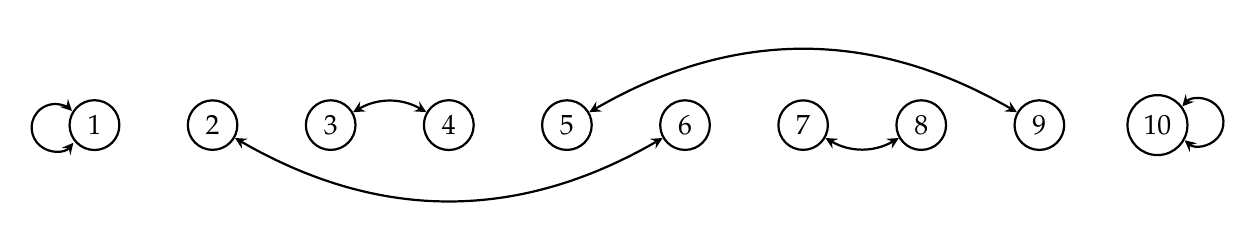
\begin{tikzpicture}[<->,>=stealth,auto,node distance=1.5cm,
  thick,main node/.style={circle,draw}]

  \node[main node] (1) {$1$};
  \draw[]	([shift=(40:-0.35cm)]1) arc (140:-135:-3mm) node[] {} (1);

  \node[main node] (2) [right of=1] {$2$};
  \node[main node] (3) [right of=2] {$3$};
  \node[main node] (4) [right of=3] {$4$};
  \node[main node] (5) [right of=4] {$5$};
  \node[main node] (6) [right of=5] {$6$};
  \node[main node] (7) [right of=6] {$7$};
  \node[main node] (8) [right of=7] {$8$};
  \node[main node] (9) [right of=8] {$9$};
  \node[main node] (10) [right of=9] {$10$};
\draw[]	(10.37) arc (138:-130:3mm) node[] {} (10);
  \path[every node/.style={font=\sffamily\small}]
    (2) edge[bend right] node[] {} (6)
    (5) edge[bend left] node[] {} (9)
    (3) edge[bend left] node[] {} (4)
    (7) edge[bend right] node[] {} (8);
\end{tikzpicture}\]

\vspace*{1.5em}

\begin{proposition}
Let $p$ be an odd prime, so $\card\Phi(p) = p-1$ is even. Then, exactly half $(=(p-1)/2)$ of $\Phi(p)$ are quadratic residues, the other half quadratic non-residues.
\end{proposition}
\begin{proof}
If $x \in \Phi(p)$, then $p\nmid x^2$, so we have a function
\[\Phi(p) \overset{f}{\longrightarrow} \Phi(p),\ x \mapsto x^2\modar{p}\]
Note that $x^2\modar{p}$ here refers to the natural representative of $x^2$ modulo $p$ in $\Phi(p)$.\\
\\
Let $R$ be the image of $f$. By definition, $R$ is the set of quadratic residues in $\Phi(p)$.\\
\begin{subproof}
\vspace*{-0.1in}
{\bf Claim.} The function $\Phi(p) \overset{f}{\longrightarrow} R$ is a two-to-one function. That is, for any $a \in R$, there exist exactly two $x_1,x_2 \in \Phi(p)$ such that $f(x_1) = a = f(x_2)$. Equivalently, $\card{f^{-1}(a)} = 2$.
\begin{proof}[Proof of Claim]
Consider the polynomial $r(T) = T^2 - \overline{a}$, for any $a \in R$, and let $y \in f^{-1}(a)$. Then $a = f(y)$, i.e. $y^2 \equiv a\modar{p}$, or equivalently $r(\overline{y}) = 0$. Therefore, $f^{-1}(a)$ consists of roots of $r(T)$.\\[0.5em]
By definition of $R$, there's atleast one $x_1 \in \Phi(p)$ such that $a = f(x_1)$, i.e. $x_1^2 \equiv a \modar{p}$, or equivalently $r(\overline{x}_1) = 0$. Now, $x_2 = p-x_1 \in \Phi(p)$ also has this property,
\begin{align*}
x_2^2 &= (p-x_1)^2\\[0.5em]
&\equiv (-x_1)^2 \modar{p}\\[0.5em]
&\equiv x_1^2\modar{p}\\[0.5em]
&\equiv a\modar{p}
\end{align*}
Since $\deg r = 2$, these two are necessarily its only roots. Furthermore, note that $x_1 \neq x_2$ as one is odd and the other even, since $x_1 + x_2 = p$, an odd prime. Hence, $\card{f^{-1}(a)} = 2$, as needed. 
\end{proof}
\vspace*{0.05ex}
\end{subproof}
\vspace*{1em}
Since $\card\Phi(p) = p-1$ and $f$ is two-to-one onto $R$. We have, $\card{R} = \dfrac{\card{\Phi(p)}}{2} = \dfrac{p-1}{2}$.
\end{proof}

\vspace*{1.5em}

\begin{definition}
Let $p$ be a prime number and $a,\,x,\,y \in \Phi(p)$. Say that $x$ and $y$ are $a$-partners if
\[xy \equiv a \modar{p}\]
\end{definition}
\emph{e.g.} Let $p = 11$,
\begin{itemize}[leftmargin=*,itemsep=2em]
\item[] $a=1$, this $1$-partnership is what we used in the proof of Theorem \ref{wilsonthm}.
\item[] $a = 2$,
\[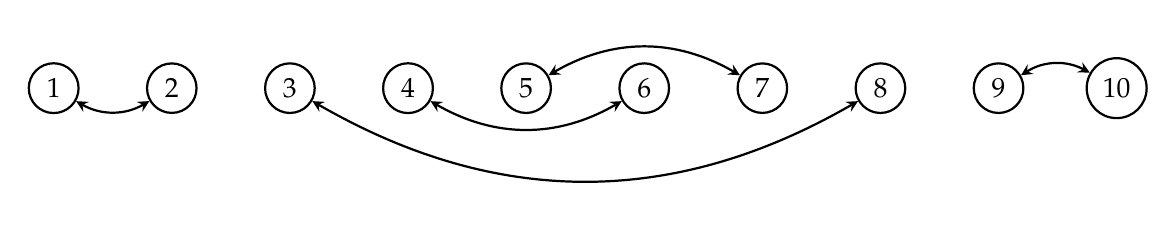
\begin{tikzpicture}[<->,>=stealth,auto,node distance=1.5cm,
  thick,main node/.style={circle,draw}]

  \node[main node] (1) {$1$};
  \node[main node] (2) [right of=1] {$2$};
  \node[main node] (3) [right of=2] {$3$};
  \node[main node] (4) [right of=3] {$4$};
  \node[main node] (5) [right of=4] {$5$};
  \node[main node] (6) [right of=5] {$6$};
  \node[main node] (7) [right of=6] {$7$};
  \node[main node] (8) [right of=7] {$8$};
  \node[main node] (9) [right of=8] {$9$};
  \node[main node] (10) [right of=9] {$10$};
  \path[every node/.style={font=\sffamily\small}]
    (1) edge[bend right] node[] {} (2)
    (3) edge[bend right] node[] {} (8)
    (5) edge[bend left] node[] {} (7)
    (9) edge[bend left] node[] {} (10)
    (4) edge[bend right] node[] {} (6);
\end{tikzpicture}\]
\item[] $a = 3$,
\[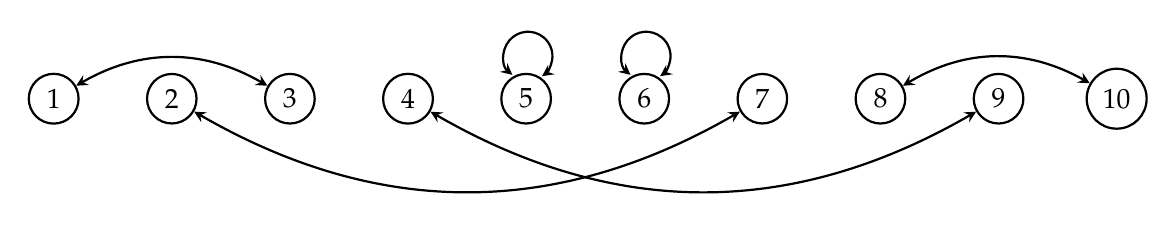
\begin{tikzpicture}[<->,>=stealth,auto,node distance=1.5cm,
  thick,main node/.style={circle,draw}]

  \node[main node] (1) {$1$};
  \node[main node] (2) [right of=1] {$2$};
  \node[main node] (3) [right of=2] {$3$};
  \node[main node] (4) [right of=3] {$4$};
  \node[main node] (5) [right of=4] {$5$};
\draw[]	([shift=(120:0.35cm)]5) arc (230:-55:3.1mm) node[] {} (5);
  \node[main node] (6) [right of=5] {$6$};
  \node[main node] (7) [right of=6] {$7$};
  \node[main node] (8) [right of=7] {$8$};
  \node[main node] (9) [right of=8] {$9$};
  \node[main node] (10) [right of=9] {$10$};
\draw[]	([shift=(120:0.35cm)]6) arc (230:-55:3.1mm) node[] {} (6);
  \path[every node/.style={font=\sffamily\small}]
    (1) edge[bend left] node[] {} (3)
    (4) edge[bend right] node[] {} (9)
    (8) edge[bend left] node[] {} (10)
    (2) edge[bend right] node[] {} (7);
\end{tikzpicture}\]
\end{itemize}

\vspace*{0.5em}

\begin{remark}
We note that every $x \in \Phi(p)$ has an $a$-partner. This is because any such $x$ has a multiplicative inverse $z$ modulo $p$, that is $xz \equiv 1 \modar{p}$. Then taking $y \in \Phi(p)$ to be such that $y \equiv az \modar{p}$ (that is, $y$ is the natural representative of $az$ modulo $p$) we have 
\[xy \equiv a(xz) \equiv a \modar{p}\]
Hence $y$ is an $a$-partner of $x$.
\end{remark}

\vspace*{1.5em}

\begin{theorem}[Euler]\label{eulerqr}
Let $p$ be an odd prime, and let $a \in \Phi(p)$. Then
\begin{itemize}
\item[(1)] $a$ is a quadratic residue if and only if $a^{\frac{p-1}{2}} \equiv 1 \modar{p}$.
\item[(2)] $a$ is a quadratic non-residue if and only if $a^{\frac{p-1}{2}} \equiv -1 \modar{p}$.
\end{itemize}
\end{theorem}
\begin{proof}
We first note that by Theorem \ref{fermatlittle} we have
\[a^{p-1} \equiv 1\modar{p}\]
Since $p$ is an odd prime, $p-1$ is even, so we get
\[(a^{\frac{p-1}{2}}-1)(a^{\frac{p-1}{2}}+1) = a^{p-1} - 1 \equiv 0\modar{p}\]
if and only if
\[a^{\frac{p-1}{2}} \equiv 1 \modar{p}\quad \text{or}\quad a^{\frac{p-1}{2}} \equiv -1 \modar{p}.\] From this, we note that the statements in the theorem are contrapositives of each other. Thus, it suffices to prove one of them; we prove (2).\\
\\
($\Leftarrow$) If $a$ is a QNR, then there's \emph{no} $x \in \Phi(p)$ that is its own $a$-partner, because otherwise we have $x^2 = x\cdot x \equiv a \modar{p}$ making $a$ a QR. Recall that every $x \in \Phi(p)$ has an $a$-partner $y \in \Phi(p)$, necessarily with $y \neq x$. Hence, by Corollary \ref{wilsonthm}, we have
\begin{align*}
-1 &\equiv (p-1)!\modar{p}\\[0.5em]
&\equiv (\text{product of elements in $\Phi(p)$})\modar{p}\\[0.5em]
&\equiv a^{\frac{p-1}{2}}\modar{p}
\end{align*}
($\Rightarrow$) Suppose $a^{\frac{p-1}{2}} \equiv -1\modar{p}$ and for the sake of contradiction assume that $a$ is a QR, then there exists an $x \in \Phi(p)$ such that $x^2 \equiv a\modar{p}$. Then
\begin{align*}
x^{p-1} &= (x^2)^{\frac{p-1}{2}}\\[0.5em]
&\equiv a^{\frac{p-1}{2}} \modar{p}\\[0.5em]
&\equiv -1 \modar{p}
\end{align*}
contradicting Corollary \ref{fermatlittle}. Thus, necessarily, $a$ is a QNR.
\end{proof}

\vspace*{1em}

\begin{remark}
Note that if $a \in \Phi(p)$ is a primitive root modulo $p$, then it's necessarily a quadratic non-residue. Since, by definition, $p-1$ is the smallest positive integer such that $a^{p-1} \equiv 1 \modar{p}$. Therefore, necessarily, $a^{\frac{p-1}{2}} \not\equiv 1 \modar{p}$. Hence, $a$ is a QNR.
\end{remark}

\vspace*{1.5em}

\begin{example} 
Determine whether $a = 3$ is a quadratic residue modulo $p = 43$.
\end{example}
\begin{proof}[Answer]
We want to compute $3^{\frac{43-1}{2}}\modar{43} = 3^{21}\modar{43}$. Note,
\allowdisplaybreaks
\begin{align*}
3^1 &\equiv 3 \modar{43}\\[0.5em]
3^2 &\equiv 9 \modar{43}\\[0.5em]
3^4 &\equiv 81 \equiv -5 \modar{43}\\[0.5em]
3^{16} &\equiv (-5)^4 \equiv 125\cdot 5 \equiv(-4)\cdot 5 \equiv-20 \modar{43}
\end{align*}
Therefore,
\begin{align*}
3^{21} = 3^{16+4+1} &\equiv (-20)\cdot (-5)\cdot 3\modar{43}\\[0.5em]
&\equiv 100\cdot 3\modar{43}\\[0.5em]
&\equiv 14\cdot 3\modar{43}\\[0.5em]
&\equiv 42\modar{43} \equiv -1\modar{43}
\end{align*}
Hence, $3$ is a QNR modulo $43$.
\end{proof}

\vspace*{1.5em}

\begin{example}[in-class]
Determine whether $a = 2$ is a quadratic residue modulo $p = 29$.
\end{example}

\vspace*{1em}

\begin{corollary}\label{qrl1}
Let $p$ be an odd prime. Then
\[-1\text{ is a quadratic residue$\modar{p}$ if and if $p \equiv 1 \modar{4}$}\]
Equivalently, $T^2 + \overline{1} \in \ff_p[T]$ is reducible if and only if $p \equiv 1 \modar{4}$.
\end{corollary}
\begin{proof}
By Theorem \ref{eulerqr}, $-1$ is a QR$\modar{p}$ if and only if
\[(-1)^{\frac{p-1}{2}} \equiv 1\modar{p}\]
Now, 
\[(-1)^{\frac{p-1}{2}} = \begin{cases}1 & \text{if $\dfrac{p-1}{2}$ is even}\\[1.5em] -1 & \text{if $\dfrac{p-1}{2}$ is odd} \end{cases}\]\\[0.2em]
Note that $\dfrac{p-1}{2}$ is even if and only if $p-1 = 4k$, for some integer $k$, if and only if $p \equiv 1 \modar{4}$.
\end{proof}

\vspace*{0.5in}

\subsection{Problems}
\vspace{0.1in}

\begin{problem}\label{Problem 16.1}
Let $p$ be an odd prime. Recall that a primitive root modulo $p$ is an integer $g$ such that \[g^{p-1} \equiv 1 \modar{p}\] and for no $0 < e < p-1$ do we have $g^e \not\equiv 1 \modar{p}$. The results that we proved in this lecture can be proved via the existence of $g$ (Theorem \ref{gaussprim}).
\begin{itemize}
\item[(a)] Consider $\ff_p^\times = \ff_p \setminus \set{\overline{0}}$ and let $g$ be a primitive root. Prove that 
\[\ff_p^\times = \setp{\overline{g}^e}{0 \leq e < p-1}\]
\item[(b)] Use a primitive root $g$ to demonstrate that $-1$ is a QR modulo $p$ if and only if $p \equiv 1 \modar{4}$.
\item[(c)] Use a primitive root $g$ to prove Theorem \ref{wilsonthm}, by first showing that
\[(p-1)! \equiv g^{1+2+\cdots+(p-2)}\modar{p}\]
\item[(d)] Given a primitive root $g$, and an integer $a$ such that $a \equiv 0 \modar{p}$, prove that $a$ is a QR modulo $p$ if and only if $a \equiv g^e \modar{p}$ for an even number $e$. Use this to prove Theorem \ref{eulerqr}.
\end{itemize} 
\end{problem}
\newpage

\section{Lecture 17 (11/23)}
\vspace*{1em}

\begin{remark}
Suppose $p$ is a prime such that $p \equiv 1 \modar{4}$, how does one find an integer $x$ such that $x^2 \equiv -1\modar{p}$? That it, a ``square root of $-1\modar{p}$".\\
\\
Consider
\begin{align*}
A &= 1\cdot 3\cdot 5\cdots (p-2)\\[0.5em]
B &= 2\cdot 4\cdot 6\cdots (p-3)\cdot (p-1)
\end{align*}
Note that the multiplicands of $B$ are negatives of the multiplicands of $A$ modulo $p$. Therefore
\[A \equiv B(-1)^{\frac{p-1}{2}} \equiv B \modar{p}\]
since $(p-1)/2$ is even. On the other hand, 
\[AB = (p-1)! \equiv -1\modar{p}\]
Hence, $A^2 \equiv AB \equiv -1\modar{p}$.\\
\\
\emph{e.g.} Let $p = 13$, then $A = 1\cdot 3\cdot 5\cdot 7\cdot 9\cdot 11 \equiv 8\modar{13}$. Then $x = 8$ is such that \[x^2 = 64 \equiv -1\modar{13}.\]
The other being $y = 13 - 8 = 5$.
\end{remark}

\vspace*{1.5em}

\begin{definition}
Let $p$ be a prime number, and $a$ an integer. Then we define the \emph{Legendre symbol} by the rule
\[\ls{a}{p} = \begin{cases}0 & \text{if $p\mid a$}\\[0.5em] 1 & \text{if $p\nmid a$ and $a$ is a QR modulo $p$}\\[0.5em] -1 & \text{if $p\nmid a$ and $a$ is a QNR modulo $p$} \end{cases}\]
{\bf Important Observation.} If $a \equiv b\modar{p}$, then
\[\ls{a}{p} = \ls{b}{p}\]
\end{definition}

\vspace*{1.5em}

We rephrase Corollary \ref{qrl1} as follows

\begin{corollary}[First Quadratic Reciprocity Law]
Let $p$ be an odd prime. Then
\begin{align*}
\ls{1}{p} &= 1,\quad \text{for any $p$}\\[1em]
\ls{-1}{p} &= \begin{cases}1 & \text{if $p\equiv 1 \modar{p}$}\\[0.5em] -1 & \text{if $p\equiv 3 \modar{4}$} \end{cases}
\end{align*}
\end{corollary}

%\vspace*{1em}

\emph{e.g.} 
\begin{itemize}
\item $\ls{3}{43} = -1$, since $3$ is a QNR modulo $43$ (we computed $3^{\frac{43-1}{2}} \equiv -1\modar{43}$).
\item $\ls{28}{29} = \ls{-1}{29} = 1$, since $29 \equiv 1 \modar{4}$.
\item $\ls{39}{13} = \ls{0}{13} = 0$.
\end{itemize}

\vspace*{1em}

Rephrasing Theorem \ref{eulerqr} using the Legendre symbol.
\begin{theorem}[Euler]\label{legeulerqr}
Let $p$ be an odd prime, and $a$ an integer. Then,
\[a^{\frac{p-1}{2}} \equiv \ls{a}{p}\modar{p}\]
Note that $1 \not\equiv -1\modar{p}$ for odd primes.
\end{theorem}

\vspace*{1.5em}

One non-trivial consequence of Theorem \ref{legeulerqr}.
\begin{corollary}
Let $p$ be an odd prime, and let $a,b$ be integers. Then
\[\ls{ab}{p} = \ls{a}{p}\ls{b}{p}\]
(the Legendre symbol is completely multiplicative). That is, $ab$ is a QR modulo $p$
\[\iff \begin{cases}\text{either \emph{both} $a$ and $b$ are QR's} & \text{(or)}\\[0.5em] \text{either \emph{both} $a$ and $b$ are QNR's} \end{cases}\]
Equivalently, $T^2 - \overline{ab} \in \ff_p[T]$ is reducible if and only if both $T^2 - \overline{a},\, T^2 - \overline{b}$ are reducible or both are irreducible.
\end{corollary}
\begin{proof}
Suppose $p\mid a$ or $p\mid b$, then $p\mid ab$. Therefore,
\[\ls{ab}{p} = 0 = \ls{a}{p}\ls{b}{p}\]
Now, suppose $p\nmid a,b$. Then by Theorem \ref{legeulerqr}, we have
\[\ls{ab}{p} \equiv (ab)^{\frac{p-1}{2}} \equiv a^{\frac{p-1}{2}}b^{\frac{p-1}{2}} \equiv \ls{a}{p}\ls{b}{p}\modar{p}\]
But necessarily, both LHS and RHS are $\pm 1$. Since $p$ is an odd prime, $1 \not\equiv -1\modar{p}$, therefore we can replace $\equiv$ with $=$ above. Thus,
\[\ls{ab}{p} = \ls{a}{p}\ls{b}{p}\]\\[-2em]
\end{proof}

%\vspace*{0.5em}

\emph{e.g.} $p = 13,\, a = 2,\, b = 6$. Note,
\begin{align*}
2^{\frac{13-1}{2}} = 2^6 = 64 &\equiv -1\modar{13};\\[0.5em]
\text{so, } \ls{2}{13} &= -1\\[1em]
6^{\frac{13-1}{2}} = 6^6 = (6^2)^3 = 36^3 &\equiv (-3)^3\modar{13}\\[0.2em]
&\equiv -27\modar{13}\\[-0.2em]
&\equiv -1\modar{13};\\[0.5em]
\text{so, } \ls{6}{13} &= -1
\end{align*}
Therefore, both $2$ and $6$ are QNR modulo $13$. On the other hand, 
\[\ls{2\cdot 6}{13} = \ls{12}{13} = \ls{-1}{13} = 1,\]
since $13 \equiv 1 \modar{4}$. Therefore,
\[\ls{2\cdot 6}{13} = 1 = (-1)^2 = \ls{2}{13}\ls{6}{13}\]

\vspace*{1.5em}

\begin{theorem}[Second Quadratic Reciprocity Law]
Let $p$ be a prime. Then
\[\ls{2}{p} = \begin{cases}0 & \text{if $p = 2$}\\[0.5em] 1 & \text{if $p\equiv \pm 1 \modar{8}$}\\[0.5em] -1 & \text{if $p\equiv \pm 3\modar{8}$} \end{cases}\]
\end{theorem}
\begin{proof}
We first note that if $p = 2$, the statement of the theorem follows from definition of the Legendre symbol. So, assume $p$ is an odd prime.\\[0.5em]
Consider the following three subproducts of $(p-1)!$
\begin{align*}
A &= 1\cdot 2\cdot 3\cdots \frac{p-3}{2}\cdot \frac{p-1}{2}\\[0.5em]
B &= 2\cdot 4\cdot 6\cdots (p-3)\cdot (p-1)\\[0.5em]
C &= 1\cdot 3\cdot 5\cdots (p-4)\cdot (p-2)
\end{align*}
There are three relations among $A,\,B$ and $C \modar{p}$
\begin{itemize}
\item[(1)] Each factor of $B$ is $2\times$ a factor of $A$. Therefore
\[B = 2^{\frac{p-1}{2}}\cdot A\]
\item[(2)] Each factor of $C$ is negative$\modar{p}$ a factor of $B$. Therefore
\[B \equiv (-1)^{\frac{p-1}{2}}\cdot C\modar{p}\]
\item[(3)] In the product of $A$, replacing each even number $x$ by $p - x \equiv -x \modar{p}$ and we will get $C$, so
\[C \equiv (-1)^{\card\text{replacements}}\cdot A\modar{p}\]
Note that,
\begin{align*}
\card\text{replacements} = \card\text{even numbers in } 1,\ldots,\frac{p-1}{2} &= \left\lfloor \frac{(p-1)/2}{2}\right\rfloor = \left\lfloor \frac{p-1}{4}\right\rfloor
\end{align*}
\end{itemize}
Letting $D$ be the multiplicative inverse of $A$ modulo $p$ (since $p\nmid A$), we summarise
\begin{align*}
B &= 2^{\frac{p-1}{2}} A \label{qr21}\tag{$1$}\\[0.5em]
2^{\frac{p-1}{2}} &\equiv BD \modar{p} \label{qr211}\tag{$1'$}\\[1em]
B&\equiv (-1)^{\frac{p-1}{2}} C\modar{p} \label{qr22}\tag{$2$}\\[1em]
C &\equiv (-1)^{\left\lfloor \frac{p-1}{4}\right\rfloor} A\modar{p} \label{qr23}\tag{$3$}\\[0.5em]
(-1)^{\left\lfloor \frac{p-1}{4}\right\rfloor} &\equiv CD \modar{p} \label{qr231}\tag{$3'$}
\end{align*}
Therefore, by Theorem \ref{legeulerqr}
\begin{align*}
\ls{2}{p} &\equiv 2^{\frac{p-1}{2}}\modar{p}\\
&\underset{\refp{qr211}}{\equiv} BD\modar{p}\\[0.5em]
&\underset{\refp{qr22}}{\equiv} (-1)^{\frac{p-1}{2}} CD\modar{p}\\[0.5em]
&\underset{\refp{qr231}}{\equiv} (-1)^{\frac{p-1}{2}}(-1)^{\left\lfloor \frac{p-1}{4}\right\rfloor}\modar{p}
\end{align*}
There are four possibilities of odd primes $p$ modulo $8,\ p\equiv 1,\,3,\,5$ or $7\modar{8}$\\
\begin{center}
{\renewcommand{\arraystretch}{2}%
\begin{tabular}{|c|c|c|c|}
\hline
$p$ & $\dfrac{p-1}{2}$ & $\left\lfloor \dfrac{p-1}{4}\right\rfloor$ & $\ls{2}{p}$\\[0.5em]
\hline
$8k + 1$ & $4k$ (even) & $2k$ (even) & $1$ \\
\hline
$8k + 2$ & $4k + 1$ (odd) & $2k$ (even) & $-1$ \\
\hline
$8k + 3$ & $4k + 2$ (even) & $2k + 1$ (odd) & $-1$ \\
\hline
$8k + 4$ & $4k + 3$ (odd) & $2k + 1$ (odd) & $1$ \\
\hline
\end{tabular}}
\end{center}
\end{proof}

%\vspace*{0.5em}

\emph{e.g.} Consider $p = 10337,\ p = 10337 \equiv 337 \equiv 17 \equiv 1 \modar{8}$. Therefore
\[\ls{2}{10337} = 1\]

\vspace*{1em}

\begin{theorem}[Gauss, Third Quadratic Reciprocity Law]
Let $p$ and $q$ be odd primes. Then
\[\ls{p}{q}\ls{q}{p} = (-1)^{\left(\frac{p-1}{2}\right)\left(\frac{q-1}{2}\right)}\]
Equivalently,
\[\ls{p}{q} = (-1)^{\left(\frac{p-1}{2}\right)\left(\frac{q-1}{2}\right)}\ls{q}{p}\]
That is, there's a tangible relation between the irreducibility of $T^2 - \overline{p} \in \ff_q[T]$ and $T^2 - \overline{q} \in \ff_p[T]$
\end{theorem}

\vspace*{1em}

{\bf Application.} Very effective way to compute $\ls{a}{p}$.\\
\\
\emph{Question.} Is $a = 3$ a quadratic residue modulo $p = 73$? That is, is the polynomial $T^2 - \overline{3} \in \ff_{73}[T]$ irreducible?
\begin{proof}[Answer]
We can employ three methods
\begin{itemize}
\item (Brute Force) Compute $x^2 \modar{73}$ for $x = 1,\ldots,72$ and see if $a = 3$ appears in the list. For a large primes ($p \sim 2^{4000}$) this is inefficient.
\item (Euler's Theorem) Compute $3^{\frac{73-1}{2}}\modar{73}$. Effective for computers.
\item (Quadratic Reciprocity)
\[\ls{3}{73} = (-1)^{\left(\frac{3-1}{2}\right)\left(\frac{73-1}{2}\right)}\ls{73}{3} = (-1)^{36}\ls{1}{3} = 1\]\\[-4em]
\end{itemize}
\end{proof}

\vspace*{1em}

Summarising
\begin{theorem}[Quadratic Reciprocity Laws]
Let $p$ be an odd prime
\begin{itemize}[itemsep=1em]
\item[(1)] $\displaystyle \ls{-1}{p} = \begin{cases}1 & \text{if $p\equiv 1 \modar{4}$}\\[0.5em] -1 & \text{if $p\equiv 3 \modar{4}$} \end{cases}$
\item[(2)] $\displaystyle \ls{2}{p} = \begin{cases} 1 & \text{if $p\equiv \pm 1\modar{8}$}\\[0.5em] -1 & \text{if $p\equiv \pm 3\modar{8}$} \end{cases}$
\item[(3)] If $q$ is an odd prime $\neq p$
\[\ls{p}{q}\ls{q}{p} = (-1)^{\left(\frac{p-1}{2}\right)\left(\frac{q-1}{2}\right)}\]
\end{itemize}
\end{theorem}

\begin{example}
Consider the polynomial $f(T) = T^2 - \overline{12}T + \overline{7} \in \ff_p[T]$. For what primes $p$ is $f(T)$ irreducible?
\end{example}
\begin{proof}[Answer]
First note that if $p = 2$, $f(T) = T^2 - \overline{12}T + \overline{7} = T^2 + \overline{1} = (T + \overline{1})^2$. Therefore $f(T)$ is reducible for $p = 2$.\\
Now, assume that $p$ is odd. Note that 
\begin{align*}
f(T) = T^2 - \overline{12}T + \overline{7} &= T^2 - \overline{2}\cdot\overline{6} T + \overline{36} - \overline{29}\\[0.5em]
&= (T - \overline{6})^2 - \overline{29}
\end{align*}
Therefore, we see that $f(T)$ has a root if and only if $f(a) = 0$ for some $a \in \ff_p$ if and only if $(a - \overline{6})^2 - \overline{29} = \overline{0}$ for some $a \in \ff_p$ if and only if $\overline{29}$ is a square modulo $p$ if and only if $29$ is a QR modulo $p$.\\
\\
Hence, by Problem \ref{Problem 13.1} and looking at the contrapositive, we have that $f(T)$ is irreducible if and only if $29$ is a QNR modulo $p$ if and only if 
\[\ls{29}{p} = -1\]
By Quadratic Reciprocity, note that
\[\ls{p}{29} = (-1)^{\left(\frac{p-1}{2}\right)\left(\frac{29-1}{2}\right)}\ls{29}{p} = (-1)^{(p-1)\cdot 7}\ls{29}{p} = \ls{29}{p}\]
since $p$ is an odd prime.\\
\\
Thus $f(T)$ is irreducible if and only if 
\[\ls{p}{29} = -1\]
Since $29$ is a prime, we have $p \equiv m \modar{29}$ for $1 \leq m \leq 28$. Checking for what such $m$ we get
\[\ls{m}{29} = -1\]
gives us our answer. 
\end{proof}

\vspace*{0.5in}

\subsection{Problems}
\vspace{0.1in}

\begin{problem}\label{Problem 17.1}
Consider the polynomial $f(T) = T^2 - \overline{6}T + \overline{4} \in \ff_p[T]$, where $p$ is a prime. In this problem, we will determine the primes for which $f(T)$ is irreducible. 
\begin{itemize}[itemsep=1em]
\item[(a)] ``Completing the square", rewrite $f$ as $(T-\overline{a})^2 - \overline{q}$ for some integer $a$ and prime $q$.
\item[(b)] Argue that $f(T)$ has no roots if and only if $q$ is a quadratic non-residue modulo $p$. Equivalently, that $f(T)$ is irreducible if and only if
\[\ls{q}{p} = -1\]
\item[(c)] Using Quadratic Reciprocity, reduce this question to determining $\ls{p}{q}$.\\
\\
Determine this by considering cases given by what $p\modar{q}$ possibly can be and other Quadratic Reciprocity Laws.
\item[(d)] Conclude. Your answer should look something like \[f(T) \text{ is irreducible if and only if }p \equiv \underline{\text{\color{white}ans}}\modar{q}.\]\\[-2em]
\end{itemize}
\end{problem}

\vspace{0.1in}

\begin{problem}\label{Problem 17.2}
If $n = 3^{e_3}5^{e_5}7^{e_7}\cdots$ is an \emph{odd} positive integer, and $a$ is an integer, the \emph{Jacobi symbol} is defined as
\[\ls{a}{n} \coloneqq \ls{a}{3}^{e_3}\cdot \ls{a}{5}^{e_5}\cdot \ls{a}{7}^{e_7}\cdots\]
where $\ls{a}{p}$ is the usual Legendre symbol. Prove the following properties.
\begin{itemize}[itemsep=1em]
\item[(a)] If $a \equiv b \modar{n}$, then $\ls{a}{n} = \ls{b}{n}$.
\item[(b)] $\ls{a}{n} = \begin{cases} 0 & \gcd(a,n) \neq 1\\[0.2em] \pm 1 & \gcd(a,n) =1 \end{cases}$.
\item[(c)] If $a,\,b$ are integers, then $\ls{a}{n}\ls{b}{n} = \ls{ab}{n}$.
\item[(d)] If $m,\,n$ are coprime odd positive integers, then
\[\ls{m}{n}\ls{n}{m} = (-1)^{\left(\frac{m-1}{2}\right)\left(\frac{n-1}{2}\right)}\]
\item[(e)] If $\ls{a}{n} = -1$ then $a$ is a quadratic non-residue modulo $n$.
\item[(f)] If $a$ is a quadratic residue modulo $n$ and $\gcd(a,n) = 1$, then $\ls{a}{n} = 1$.
\end{itemize}
Unlike the Legendre symbol, if $\ls{a}{n} = 1$ then $a$ may not be a quadratic residue modulo $n$.
\end{problem}
\newpage

\section{Lecture 18 (11/30)}
\vspace*{1em}

\begin{example}
For which primes $p$ is $3$ a quadratic residue modulo $p$?
\end{example}
\begin{proof}[Answer]
Note that $3$ is a QR mod $p$ for $p = 2$ and $p =3$. Therefore, now assume the prime $p > 3$ and then Quadratic Reciprocity gives us
\begin{align*}
\ls{3}{p} &= (-1)^{\left(\frac{3-1}{2}\right)\left(\frac{p-1}{2}\right)}\ls{p}{3}\\[0.5em]
&= (-1)^{\frac{p-1}{2}}\ls{p}{3}\\[1em]
&= \ls{p}{3}\cdot\left(\begin{array}{l}
1 \qquad \text{if } p \equiv 1 \modar{4}\\[1em]
-1 \quad\ \ \!\!\text{if } p \equiv -1 \modar{4}
\end{array} \right)
\end{align*}
Note that
\[\ls{p}{3} = \begin{cases} \ls{1}{3} = 1 & \text{if } p \equiv 1 \modar{3}\\[1.5em]
 \ls{-1}{3} = -1 & \text{if } p \equiv -1 \modar{3}\end{cases}\]
Therefore
\begin{align*}
\ls{3}{p} &= \begin{cases}
1\cdot 1 & \text{if } p \equiv [1,1] \modar{[3,4]}\\[0.5em]
(-1)\cdot (-1) & \text{if } p \equiv [-1,-1] \modar{[3,4]}\\[0.5em]
(-1)\cdot 1 & \text{if } p \equiv [-1,1] \modar{[3,4]}\\[0.5em]
1\cdot (-1) & \text{if } p \equiv [1,-1] \modar{[3,4]}
\end{cases}\\[1.5em]
&= \begin{cases}
1 & \text{if } p \equiv [1,1] \modar{[3,4]}\\[0.5em]
1 & \text{if } p \equiv [-1,-1] \modar{[3,4]}\\[0.5em]
-1 & \text{if } p \equiv [5,5] \modar{[3,4]}\\[0.5em]
-1 & \text{if } p \equiv [-5,-5] \modar{[3,4]}
\end{cases}
\end{align*}
\vspace{0.1in}\\
Putting these congruences together via CRT (Remark \ref{crtprac}), we find that\\
\[\ls{3}{p} = \begin{cases} 1 & \text{if } p \equiv \pm 1 \modar{12} \text{ or } p=2\\[0.75em]
-1 & \text{if } p \equiv \pm 5 \modar{12}\end{cases}\]\\
For example, the smallest odd prime for which $3$ is a quadratic residue is $11$, since $11 \equiv -1 \modar{12}$,
\[6^2\equiv 5^2 \equiv 3 \modar{11},\]
and the smallest prime for which $3$ is a quadratic non-residue is $7$, since $7 \equiv -5 \modar{12}$
\end{proof}

%\vspace*{1.5em}

\begin{example}
Does the equation
\[x^2 = 59783y + 46,\quad 59783 = 191\cdot 313\]
have any integer solutions?
\end{example}
\begin{proof}[Answer]
We have the following steps
\begin{itemize}[leftmargin=3.3em,itemsep=2em]
\item[\emph{Step 1.}] Division algorithm is very useful for linear equations, but this is a quadratic equation.
\item[\emph{Step 2.}] Reducing$\modar{59783}$, we ask if 
\[x^2 \equiv 46\modar{59783}\]
has an integer solution.
\item[\emph{Step 3.}] By CRT, $x^2 \equiv 46\modar{59783}$ has a solution if and only if
\begin{align*}[left=\empheqlbrace]
x^2 &\equiv 46\modar{191};\ \text{and}\label{eqc1}\tag{$1$}\\[0.1em]
x^2 &\equiv 29\modar{313}\label{eqc2}\tag{$2$}
\end{align*}
have solutions.
\item[\emph{Step 4.}] So, we look to see if \refp{eqc1} and \refp{eqc2} have an intger solutions, that is, compute
\[\ls{46}{191}\quad \text{and}\quad \ls{46}{313}\]
\item[\emph{Step 5.}] $\displaystyle \ls{46}{191} = \ls{2}{191}\ls{23}{191}$. Note that
\begin{align*}
\ls{2}{191} &= 1,\quad \text{since }191 \equiv 7\modar{8}\\[1em]
\ls{23}{191} &= (-1)^{\left(\frac{23-1}{2}\right)\left(\frac{191-1}{2}\right)}\ls{191}{23}\\[0.5em]
&= (-1)\ls{7}{23}\\[0.5em]
&= (-1)(-1)^{\left(\frac{7-1}{2}\right)\left(\frac{23-1}{2}\right)}\ls{23}{7}\\[0.5em]
&= (-1)^2\ls{2}{7}\\[0.5em]
&= 1
\end{align*}
So, $\ls{46}{191} = 1\cdot 1 = 1$. Therefore \refp{eqc1} has a solution.
\item[\emph{Step 6.}] $\displaystyle \ls{46}{313} = \ls{2}{313}\ls{23}{313}$. Note that
\begin{align*}
\ls{2}{313} &= 1,\quad \text{since }313 \equiv 1\modar{8}\\[1em]
\ls{23}{313} &= (-1)^{\left(\frac{23-1}{2}\right)\left(\frac{313-1}{2}\right)}\ls{313}{23}\\[0.5em]
&= \ls{14}{23}\\[0.5em]
&= \ls{2}{23}\ls{7}{23}\\[0.5em]
&= 1(-1)\\[0.5em]
&= -1
\end{align*}
So, $\ls{46}{313} = -1$. Therefore \refp{eqc2} does not have a solution.
\end{itemize}
\vspace*{0.2in}
Hence $x^2 \equiv 46 \modar{59783}$ has no integer solutions. Thus
\[x^2 = 59783y + 46\]
has no integer solutions.
\end{proof}

\vspace*{5em}

{\bf An Application of the Quadratic Reciprocity Law. Fermat's Christmas Theorem}

\begin{theorem}[Fermat's Christmas Theorem]\label{fermchr}
Let $p$ be a prime such that $p \equiv 1 \modar{p}$. Then the equation
\[p = x^2 + y^2\]
has integer solutions. That is, $p$ can be written as a sum of two squares.\\[0.5em]
(this appears in Fermat's letter to Mersenne dated $25^{\text{th}}$ Dec, 1640)\\
\\
{\bf Examples and Remarks.}
\begin{itemize}
\item $13 = 2^2 + 3^2$ and $17 = 4^2 + 1^2$
\item $p=2,\ 2 = 1^2 + 1^2$
\item Suppose $p \equiv 3\modar{4}$. Then $p$ cannot be written as a sum of two squares, since for integers $x,y$ we have $x^2 + y^2 \equiv 0,1,2 \modar{4}$ as we saw some time ago.
\item We consider the set $\zz[i] = \setp{a + bi}{a,b \in \zz}$, what we have then is that if $p \equiv 1 \modar{4}$, then $p = (x+iy)(x-iy)$ in the set $\zz[i]$.
\end{itemize}
\end{theorem}

%\vspace*{1.5em}

{\bf Some Geometric Preliminaries} (Minkowski).\\[0.5em]
We ask a general question,\\[0.5em]
Consider a lattice (a grid of parallelograms in the plane); more precisely, fix the two non-parallel vector $\vec{v},\,\vec{w}$ and consider
\[L = \setp{a\vec{v}+b\vec{w}}{a,b \in \zz}\]
associated is the fundamental parallelogram, given as \[\Pi_L = \setp{m\vec{v}+n\vec{w}}{m,n \in [0,1]}.\]\\
\emph{e.g.}
\[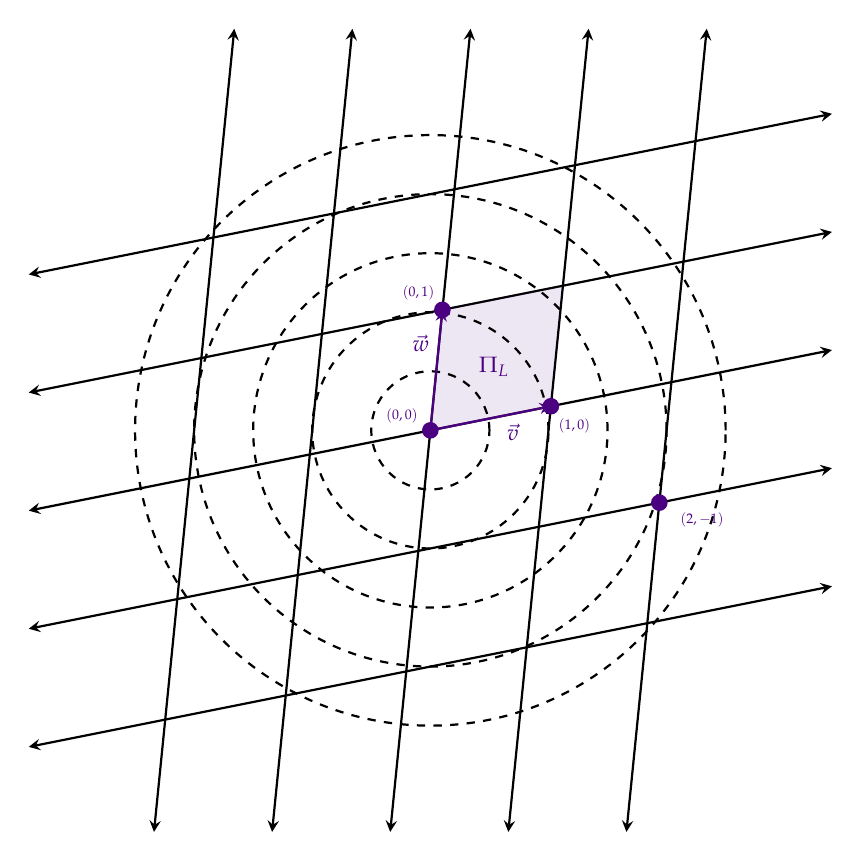
\begin{tikzpicture}[scale=3]
    \draw[<->,thick,>=stealth] (0.83,-1.7)--(1.17,1.7);
    \draw[<->,thick,>=stealth] (0.33,-1.7)--(0.67,1.7);
    \draw[<->,thick,>=stealth] (-0.17,-1.7)--(0.17,1.7);
    \draw[<->,thick,>=stealth] (-0.67,-1.7)--(-0.33,1.7);
    \draw[<->,thick,>=stealth] (-1.17,-1.7)--(-0.83,1.7);
%-----------------------------------------------
    \draw[<->,thick,>=stealth] (-1.7,0.66)--(1.7,1.34);
    \draw[<->,thick,>=stealth] (-1.7,0.16)--(1.7,0.84);
    \draw[<->,thick,>=stealth] (-1.7,-0.34)--(1.7,0.34);
    \draw[<->,thick,>=stealth] (-1.7,-0.84)--(1.7,-0.16);
    \draw[<->,thick,>=stealth] (-1.7,-1.34)--(1.7,-0.66);
%-----------------------------------------------
    \coordinate (a) at (0,0);
    \coordinate (b) at (0.051,0.5102);
    \coordinate (c) at (0.5612,0.6122);
    \coordinate (d) at (0.5102,0.102);
    \fill [indigo, fill opacity=1/10] 
        (a) -- (b) -- (c) -- (d) -- cycle;
%-----------------------------------------------
    \draw[thick,dashed](0,0) circle (0.25);
    \draw[thick,dashed](0,0) circle (0.5);
    \draw[thick,dashed](0,0) circle (0.75);
    \draw[thick,dashed](0,0) circle (1);
    \draw[thick,dashed](0,0) circle (1.25);
%-----------------------------------------------
    \fill[color=indigo] (0,0) circle (1pt);
    \fill[color=indigo] (0.051,0.5102) circle (1pt);
    \fill[color=indigo] (0.5102,0.102) circle (1pt);
%    \fill[color=indigo] (0.5612,0.6122) circle (1pt);
    \fill[color=indigo] (0.9694,-0.3061) circle (1pt);
%-----------------------------------------------
    \draw[->,thick,>=stealth,color=indigo] (0,0)--(0.051,0.5102);
    \draw[->,thick,>=stealth,color=indigo] (0,0)--(0.5102,0.102);
%-----------------------------------------------
	\node[color=indigo] at (0.35,-0.01) {\footnotesize$\vec{v}$};
    \node[color=indigo] at (-0.04,0.37) {\footnotesize $\vec{w}$};
    \node[color=indigo] at (1.15,-0.38) {\tiny $(2,-1)$};
    \node[color=indigo] at (-0.12,0.06) {\tiny $(0,0)$};
    \node[color=indigo] at (0.61,0.02) {\tiny $(1,0)$};
    \node[color=indigo] at (-0.05,0.58) {\tiny $(0,1)$};
    \node[color=indigo] at (0.27,0.27) {\footnotesize $\Pi_L$};
\end{tikzpicture}\]\\
Now, consider $C_r$'s, circles of radius $r$ centred at the origin. 
\begin{itemize}
\item If $r$ is very small, the only grid point contained in the circle will be the origin.
\item If $r$ is sufficiently large, the circle will contain grid points other than the origin.
\end{itemize}
%\vspace*{1em}
\emph{Question.} When (in terms of $r$) can we be sure that a circle of radius $r$ centred at the origin contains a grid point other than the origin?\\[1em]
A possible answer can be to take $r > \min\set{|\vec{v}|,|\vec{w}|}$; a more useful characterization, for the purposes of proving Theorem \ref{fermchr}, is given as following.

\vspace*{1.5em}

\begin{theorem}[Minkwoski]\label{mink}
If $\mathrm{Area}(C_r) = \pi r^2 > 4\cdot\mathrm{Area}(\Pi_L)$, then $C_r$ contains at least one grid point different from the origin.
\end{theorem}
\begin{proof}
Suppose $\pi r^2 > 4\cdot\mathrm{Area}(\Pi_L)$. The grid divides $C_r$ into four sectors, which we label $A,\,B,\,C$ and $D$. An example is illustrated below.
\[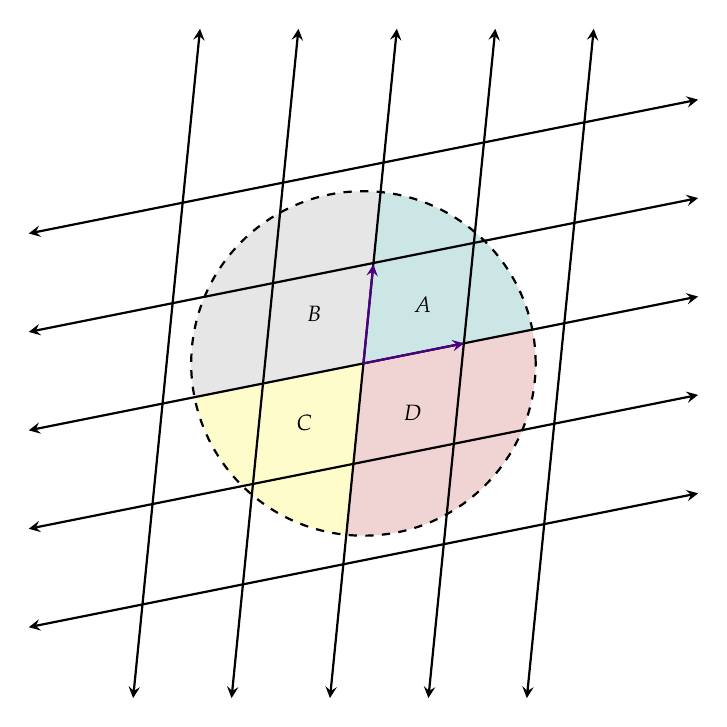
\begin{tikzpicture}[scale=2.5]
    \fill[teal, fill opacity=1/5] (0,0) -- +(84.3:0.875) arc (84.3:11.31:0.875);
    \fill[firebrick, fill opacity=1/5] (0,0) -- +(11.31:0.875) arc (11.31:-95.7:0.875);
    \fill[yellow, fill opacity=1/5] (0,0) -- +(-95.7:0.875) arc (-95.7:-168.69:0.875);
    \fill[gray, fill opacity=1/5] (0,0) -- +(-168.69:0.875) arc (-168.69:-275.7:0.875);
%-----------------------------------------------
    \draw[<->,thick,>=stealth] (0.83,-1.7)--(1.17,1.7);
    \draw[<->,thick,>=stealth] (0.33,-1.7)--(0.67,1.7);
    \draw[<->,thick,>=stealth] (-0.17,-1.7)--(0.17,1.7);
    \draw[<->,thick,>=stealth] (-0.67,-1.7)--(-0.33,1.7);
    \draw[<->,thick,>=stealth] (-1.17,-1.7)--(-0.83,1.7);
%-----------------------------------------------
    \draw[<->,thick,>=stealth] (-1.7,0.66)--(1.7,1.34);
    \draw[<->,thick,>=stealth] (-1.7,0.16)--(1.7,0.84);
    \draw[<->,thick,>=stealth] (-1.7,-0.34)--(1.7,0.34);
    \draw[<->,thick,>=stealth] (-1.7,-0.84)--(1.7,-0.16);
    \draw[<->,thick,>=stealth] (-1.7,-1.34)--(1.7,-0.66);
%-----------------------------------------------
    \draw[->,thick,>=stealth,color=indigo] (0,0)--(0.0503,0.5025);
    \draw[->,thick,>=stealth,color=indigo] (0,0)--(0.5102,0.102);
%-----------------------------------------------
    \draw[thick,dashed](0,0) circle (0.875);%-----------------------------------------------
	\node[] at (0.3,0.3) {\footnotesize$A$};
    \node[] at (-0.25,0.25) {\footnotesize $B$};
    \node[] at (-0.3,-0.3) {\footnotesize $C$};
    \node[] at (0.25,-0.25) {\footnotesize $D$};
\end{tikzpicture}\]
Let's now do the following
\begin{itemize}
\item Translate the sector $B$ by $2\vec{v}$,\quad $B + 2\vec{v} = \{\vec{b} + 2\vec{v}\ :\ \vec{b}\in B\}$
\item Translate the sector $D$ by $2\vec{w}$,\quad $D + 2\vec{w} = \{\vec{d} + 2\vec{w}\ :\ \vec{d}\in D\}$
\item Translate the sector $C$ by $2\vec{v} + 2\vec{w}$,\quad $C + 2\vec{v} + 2\vec{w} = \setp{\vec{c} + 2\vec{v} + 2\vec{w}}{\vec{c}\in C}$.
\end{itemize}
The straight edges of the sectors are now against the sides of the parallelogram, $\Pi'$, given by $2\vec{v}$ and $2\vec{w}$.
\[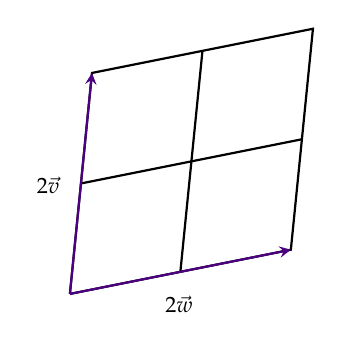
\begin{tikzpicture}[scale=2.75]
%-----------------------------------------------
    \draw[thick] (0,0)--(0.102,1.0204)--(1.1224,1.2245)--(1.0204,0.2041)--(0,0);
    \draw[thick] (0.5102,0.102)--(0.6122,1.1224);
    \draw[thick] (0.051,0.5102)--(1.0714,0.7143);
%-----------------------------------------------
    \draw[->,thick,>=stealth,color=indigo] (0,0)--(0.102,1.0204);
    \draw[->,thick,>=stealth,color=indigo] (0,0)--(1.0204,0.2041);
%-----------------------------------------------
	\node[] at (-0.1,0.5) {\footnotesize$2\vec{v}$};
    \node[] at (0.5047,-0.05) {\footnotesize $2\vec{w}$};
\end{tikzpicture}
\qquad\qquad
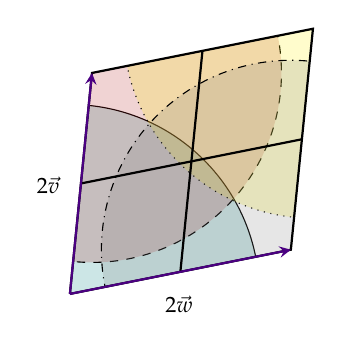
\begin{tikzpicture}[scale=2.75]
    \draw[fill=teal, fill opacity=1/5] (0,0) -- +(84.3:0.875) arc (84.3:11.31:0.875);
    \draw[dashed,fill=firebrick, fill opacity=1/5] (0.102,1.0204) -- +(11.31:0.875) arc (11.31:-95.7:0.875);
    \draw[dotted,fill=yellow, fill opacity=1/5] (1.1224,1.2245) -- +(-95.7:0.875) arc (-95.7:-168.69:0.875);
    \draw[dashdotted,fill=gray, fill opacity=1/5] (1.0204,0.2041) -- +(-168.69:0.875) arc (-168.69:-275.7:0.875);
%-----------------------------------------------
    \draw[thick] (0,0)--(0.102,1.0204)--(1.1224,1.2245)--(1.0204,0.2041)--(0,0);
    \draw[thick] (0.5102,0.102)--(0.6122,1.1224);
    \draw[thick] (0.051,0.5102)--(1.0714,0.7143);
%-----------------------------------------------
    \draw[->,thick,>=stealth,color=indigo] (0,0)--(0.102,1.0204);
    \draw[->,thick,>=stealth,color=indigo] (0,0)--(1.0204,0.2041);
%-----------------------------------------------
	\node[] at (-0.1,0.5) {\footnotesize$2\vec{v}$};
    \node[] at (0.5047,-0.05) {\footnotesize $2\vec{w}$};
\end{tikzpicture}\]
Since $\mathrm{Area}(\Pi') = 4\cdot \mathrm{Area}(\Pi_L) < \pi r^2 = \mathrm{Area}(A) + \mathrm{Area}(B) + \mathrm{Area}(C) + \mathrm{Area}(D)$, by assumption. The sectors must overlap within $\Pi'$. Illustrated above.\\
\\
Therefore, atleast two of the four (translated) sectors should intersect. Hence, we have $\binom{4}{2} = 6$ possibilities.\\
\\
\emph{Case I.} Suppose $A$ and $D + 2\vec{w}$ intersect. Then there exists a $P \in A$ and $Q \in D$ such that $P = Q + 2\vec{w}$. Therefore $\vec{w} = (P-Q)/2$. Since $P,Q \in C_r$ and $C_r$ is convex, we get $\vec{w} \in C_r$.\\
\\
The remaining five cases are handled similarly.
\end{proof}

%\vspace*{1.5em}

\begin{proof}[Proof of Fermat's Christmas Theorem (Theorem \ref{fermchr})]
Let $p$ be a prime such that $p \equiv 1 \modar{p}$. By the First Quadratic Reciprocity Law, we know $-1$ is a QR modulo $p$. So, there exists an integer $n$ such that $n^2 \equiv -1 \modar{p}$.\\
\\
Consider the set $L = \setp{(x,y) \in \zz^2}{x \equiv ny \modar{p}}$.\\[0.5em]
\begin{subproof}
%\vspace*{-0.1in}
{\bf Claim.} $L$ is a lattice. More precisely, any $(x,y) \in S$ can be uniquely written as
\[(x,y) = a\underbrace{(n,1)}_{\vec{v}} + b\underbrace{(p,0)}_{\vec{w}},\quad \text{for some } a,b \in \zz\]
and conversely, for any $a,b \in \zz$, we have $a\vec{v} + b\vec{w} \in L$.
\begin{proof}[Proof of Claim]
If $(x,y) \in L$, then $x \equiv ny \modar{p}$, i.e. $x = ny + pz$ for some integer $z$. Take $a = y$ and $b = z$. Then,
\[a(n,1) + b(p,0) = y(n,1) + z(p,0) = (ny,y) + (pz,0) = (ny + pz,y) = (x,y),\]
as needed.\\
\\
Conversely, for any $a,b \in \zz$, consider
\[(x,y) = a\vec{v} + b\vec{w} = (an + bp,a);\]
i.e. $x = an + bp$ and $y = a$. Therefore, $x = an + bp \equiv na\equiv ny \modar{p}$. Hence, $(x,y) \in L$.
\end{proof}
\vspace*{0.05ex}
\end{subproof}
\vspace*{1.5em}
Now, $L$ is a lattice spanned by $\vec{v} = (n,1)$ and $\vec{w} = (p,0)$. Therefore, 
\[\mathrm{Area}(\Pi_L) = \abs{\det(\vec{v},\vec{w})} = \abs{\det\begin{pmatrix}n & p\\ 1 & 0 \end{pmatrix}} = p\]
Let's consider the circle of area $4p + \epsilon$ for some small $\epsilon > 0$. Hence, we have considered $C_r$ with
\[r = \sqrt{\frac{4p + \epsilon}{\pi}}\]
By design, we have $\mathrm{Area}(C_r) > 4\cdot\mathrm{Area}(\Pi_L)$, thus by Theorem \ref{mink} there exists an $(x,y) \in L$ with $(x,y) \neq (0,0)$ such that it's contained in $C_r$. Therefore
\begin{align*}
0 < x^2 + y^2 < r^2 = \frac{4p + \epsilon}{\pi}, &\quad \text{since }(x,y) \in \text{interior of }C_r\\[0.5em]
x \equiv ny \modar{p}, &\quad \text{since }(x,y) \in L
\end{align*}
We have $x^2 \equiv n^2y^2 \equiv - y^2 \modar{p}$, since $n^2 \equiv -1\modar{p}$. Hence, $x^2 + y^2 \equiv 0 \modar{p}$; in particular, $(x^2 + y^2)/p \in \zz$.\\
\\
Now, note that
\[0 < \frac{x^2 + y^2}{p} < \frac{1}{p}\cdot \frac{4p + \epsilon}{\pi} = \frac{4}{\pi} + \frac{\epsilon}{\pi p}\]
Since our choice of $\epsilon$ was arbitrary, we can choose an $\epsilon$, for example $\epsilon < \pi p/2$, to get
\[\frac{4}{\pi} + \frac{\epsilon}{\pi p}< 2\]
Thus, 
\[0 < \frac{x^2 + y^2}{p} < 2\]
Necessarily, $\dfrac{x^2 + y^2}{p} = 1$, and therefore $p = x^2 + y^2$.
\end{proof}

\vspace*{1.5em}

\begin{remark}
Let $\Sigma_2 = \setp{x \in \zz}{x = a^2 + b^2,\ \text{for some $a,b \in \zz$}}$, that is the set of integers that can be written as a sum of two squares. Theorem \ref{fermchr} tells us that a prime $p \in \Sigma_2$ if and only if $p\equiv 1 \modar{4}$.\\
\\
Now, one can verify the following identity quickly
\[(a^2 + b^2)(c^2 + d^2) = (ac-bd)^2 + (ad + bc)^2;\]
which tell us that if $x,\,y \in \Sigma_2$, then $xy \in \Sigma_2$.\\
\\
Noting that if a prime $q \equiv 3\modar{4}$ then $q \notin \Sigma_2$, we get a complete description of $\Sigma_2$. 
\[x \in \Sigma_2 \iff \text{every prime $q \equiv 3 \modar{4}$ divides $x$ to an even power (take it to be $0$ if $q\nmid x$)}\]
\emph{e.g.} The integer $60 = 2^2\cdot 3\cdot 5$ is not a sum of two squares, since the exponent of $3$ dividing it is odd.\\
\\
However, $180 = 2^2\cdot 3^2\cdot 5$ is a sum of two squares. To find them, first write $5$ as a sum of two squares: $5 = 2^2 + 1^2$. Now multiplying through by $2^2\cdot 3^2$ we get \[180 = 2^2\cdot 3^2\cdot 5 = (2\cdot 3\cdot 2)^2 + (2\cdot 3\cdot 1)^2 = 12^2 + 6^2.\]
\end{remark}

\vspace*{1.5em}

\begin{remark}
Initiating a set-up similar to the one we had while proving Theorem \ref{fermchr}, this time in $\rr^3$, and using a version of Theorem \ref{mink} in three dimensions, again by Minkowski, allows us to prove the following celebrated theorem.
\begin{theorem*}[Lagrange's Four-Square Theorem]
Any positive integer $n$ can be expressed as a sum of four squares. That is, there exist integers $x,\,y,\,z$ and $w$ such that 
\[n = x^2 + y^2 + z^2 + w^2\]
\end{theorem*} 
%\vspace*{1em}
%A natural follow-up question to ask is: how many ways can a positive integer $n$ be written as a sum of four squares. This question has a complete answer which, surprisingly, is completely intrinsic to $n$.\\
%\\
%Define 
%\[r_4(n) = \setp{(x,y,z,w) \in \zz^4}{x^2 + y^2 + z^2 + w^2 = n};\]
%that is, $r_4(n)$ is the number of ways $n$ can be written as a sum of four squares.
%\begin{theorem*}[Jacobi's Four-Square Theorem]
%For a positive integer $n$,
%\[r_4(n) = 8\cdot\left(\sum_{d \in \mathscr{D}(n),\, 4\nmid d}d\right) = 8\sigma_1(n) - 32\sigma_1(n/4)\]
%where $\sigma_1(n/4) = 0$ if $4\nmid n$.\\[1em]
%In particular, for a prime $p$, $r_4(p) = 8(p+1)$.
%\end{theorem*} 
\end{remark}

\vspace*{0.5in}

\subsection{Problems}
\vspace{0.1in}

\begin{problem}\label{Problem 18.1}
For which primes $p$ is $5$ a quadratic residue modulo $p$?
\end{problem}
\newpage
%
%\section{Lecture 19 (12/2)}
%\vspace*{1em}

Rephrasing Theorem \ref{eulerqr} using the Legendre symbol.
\begin{theorem}[Euler]\label{legeulerqr}
Let $p$ be an odd prime, and $a$ an integer. Then,
\[a^{\frac{p-1}{2}} \equiv \ls{a}{p}\modar{p}\]
Note that $1 \not\equiv -1\modar{p}$ for odd primes.
\end{theorem}

\vspace*{1em}

One non-trivial consequence of Theorem \ref{legeulerqr}.
\begin{corollary}
Let $p$ be an odd prime, and let $a,b$ be integers. Then
\[\ls{ab}{p} = \ls{a}{p}\ls{b}{p}\]
(the Legendre symbol is completely multiplicative). That is, $ab$ is a QR modulo $p$
\[\iff \begin{cases}\text{either \emph{both} $a$ and $b$ are QR's} & \text{(or)}\\[0.5em] \text{either \emph{both} $a$ and $b$ are QNR's} \end{cases}\]
Equivalently, $T^2 - \overline{ab} \in \ff_p[T]$ is reducible if and only if both $T^2 - \overline{a},\, T^2 - \overline{b}$ are reducible or both are irreducible.
\end{corollary}
\begin{proof}
Suppose $p\mid a$ or $p\mid b$, then $p\mid ab$. Therefore,
\[\ls{ab}{p} = 0 = \ls{a}{p}\ls{b}{p}\]
Now, suppose $p\nmid a,b$. Then by Theorem \ref{legeulerqr}, we have
\[\ls{ab}{p} \equiv (ab)^{\frac{p-1}{2}} \equiv a^{\frac{p-1}{2}}b^{\frac{p-1}{2}} \equiv \ls{a}{p}\ls{b}{p}\modar{p}\]
But necessarily, both LHS and RHS are $\pm 1$. Since $p$ is an odd prime, $1 \not\equiv -1\modar{p}$, therefore we can replace $\equiv$ with $=$ above. Thus,
\[\ls{ab}{p} = \ls{a}{p}\ls{b}{p}\]
\end{proof}

\vspace*{0.5em}

\emph{e.g.} $p = 13,\, a = 2,\, b = 6$. Note,
\begin{align*}
2^{\frac{13-1}{2}} = 2^6 = 64 &\equiv -1\modar{13}; & \text{so, } \ls{2}{13} &= -1\\[0.5em]
6^{\frac{13-1}{2}} = 6^6 = (6^2)^3 = 36^3 &\equiv (-3)^3\modar{13}\\[0.2em]
&\equiv -27\modar{13}\\[-0.2em]
&\equiv -1\modar{13}; & \text{so, } \ls{6}{13} &= -1
\end{align*}
Therefore, both $2$ and $6$ are QNR modulo $13$. On the other hand, 
\[\ls{2\cdot 6}{13} = \ls{12}{13} = \ls{-1}{13} = 1,\]
since $13 \equiv 1 \modar{4}$. Therefore,
\[\ls{2\cdot 6}{13} = 1 = (-1)^2 = \ls{2}{13}\ls{6}{13}\]

\vspace*{1em}

\begin{theorem}[Second Quadratic Reciprocity Law]
Let $p$ be a prime. Then
\[\ls{2}{p} = \begin{cases}0 & \text{if $p = 2$}\\[0.5em] 1 & \text{if $p\equiv \pm 1 \modar{8}$}\\[0.5em] -1 & \text{if $p\equiv \pm 3\modar{8}$} \end{cases}\]
\end{theorem}
\begin{proof}
We first note that if $p = 2$, the statement of the theorem follows from definition of the Legendre symbol. So, assume $p$ is an odd prime.\\
\\
Consider the following three subproducts of $(p-1)!$
\begin{align*}
A &= 1\cdot 2\cdot 3\cdots \frac{p-3}{2}\cdot \frac{p-1}{2}\\[0.5em]
B &= 2\cdot 4\cdot 6\cdots (p-3)\cdot (p-1)\\[0.5em]
C &= 1\cdot 3\cdot 5\cdots (p-4)\cdot (p-2)
\end{align*}
There are three relations among $A,\,B$ and $C \modar{p}$
\begin{itemize}
\item[(1)] Each factor of $B$ is $2\times$ a factor of $A$. Therefore
\[B = 2^{\frac{p-1}{2}}\cdot A\]
\item[(2)] Each factor of $C$ is negative$\modar{p}$ a factor of $B$. Therefore
\[B \equiv (-1)^{\frac{p-1}{2}}\cdot C\modar{p}\]
\item[(3)] In the product of $A$, replacing each even number $x$ by $p - x \equiv -x \modar{p}$ and we will get $C$, so
\[C \equiv (-1)^{\card\text{replacements}}\cdot A\modar{p}\]
Note that,
\begin{align*}
\card\text{replacements} = \card\text{even numbers in } 1,\ldots,\frac{p-1}{2} &= \left\lfloor \frac{(p-1)/2}{2}\right\rfloor\\[0.5em]
&= \left\lfloor \frac{p-1}{4}\right\rfloor
\end{align*}
\end{itemize}
Letting $D$ be the multiplicative inverse of $A$ modulo $p$ (since $p\nmid A$), we summarise
\begin{align*}
B &= 2^{\frac{p-1}{2}} A \label{qr21}\tag{$1$}\\[0.5em]
2^{\frac{p-1}{2}} &\equiv BD \modar{p} \label{qr211}\tag{$1'$}\\[1em]
B&\equiv (-1)^{\frac{p-1}{2}} C\modar{p} \label{qr22}\tag{$2$}\\[1em]
C &\equiv (-1)^{\left\lfloor \frac{p-1}{4}\right\rfloor} A\modar{p} \label{qr23}\tag{$3$}\\[0.5em]
(-1)^{\left\lfloor \frac{p-1}{4}\right\rfloor} &\equiv CD \modar{p} \label{qr231}\tag{$3'$}
\end{align*}
Therefore, by Theorem \ref{legeulerqr}
\begin{align*}
\ls{2}{p} &\equiv 2^{\frac{p-1}{2}}\modar{p}\\
&\underset{\refp{qr211}}{\equiv} BD\modar{p}\\[0.5em]
&\underset{\refp{qr22}}{\equiv} (-1)^{\frac{p-1}{2}} CD\modar{p}\\[0.5em]
&\underset{\refp{qr231}}{\equiv} (-1)^{\frac{p-1}{2}}(-1)^{\left\lfloor \frac{p-1}{4}\right\rfloor}\modar{p}
\end{align*}
There are four possibilities of odd primes $p$ modulo $8,\ p\equiv 1,\,3,\,5$ or $7\modar{8}$\\
\begin{center}
{\renewcommand{\arraystretch}{2}%
\begin{tabular}{|c|c|c|c|}
\hline
$p$ & $\dfrac{p-1}{2}$ & $\left\lfloor \dfrac{p-1}{4}\right\rfloor$ & $\ls{2}{p}$\\[0.5em]
\hline
$8k + 1$ & $4k$ (even) & $2k$ (even) & $1$ \\
\hline
$8k + 2$ & $4k + 1$ (odd) & $2k$ (even) & $-1$ \\
\hline
$8k + 3$ & $4k + 2$ (even) & $2k + 1$ (odd) & $-1$ \\
\hline
$8k + 4$ & $4k + 3$ (odd) & $2k + 1$ (odd) & $1$ \\
\hline
\end{tabular}}
\end{center}
\end{proof}

\vspace*{0.5em}

\emph{e.g.} Consider $p = 10337,\ p = 10337 \equiv 337 \equiv 17 \equiv 1 \modar{8}$. Therefore
\[\ls{2}{10337} = 1\]

\vspace*{1em}

\begin{theorem}[Gauss, Third Quadratic Reciprocity Law]
Let $p$ and $q$ be odd primes. Then
\[\ls{p}{q}\ls{q}{p} = (-1)^{\left(\frac{p-1}{2}\right)\left(\frac{q-1}{2}\right)}\]
Equivalently,
\[\ls{p}{q} = (-1)^{\left(\frac{p-1}{2}\right)\left(\frac{q-1}{2}\right)}\ls{q}{p}\]
That is, there's a tangible relation between the irreducibility of $T^2 - \overline{p} \in \ff_q[T]$ and $T^2 - \overline{q} \in \ff_p[T]$
\end{theorem}

\vspace*{1em}

{\bf Application.} Very effective way to compute $\ls{a}{p}$.\\
\\
\emph{Question.} Is $a = 3$ a quadratic residue modulo $p = 73$? That is, is the polynomial $T^2 - \overline{3} \in \ff_{73}[T]$ irreducible?
\begin{proof}[Answer]
We can employ three methods
\begin{itemize}
\item (Brute Force) Compute $x^2 \modar{73}$ for $x = 1,\ldots,72$ and see if $a = 3$ appears in the list. For a large primes ($p \sim 2^{4000}$) this is inefficient.
\item (Euler's Theorem) Compute $3^{\frac{73-1}{2}}\modar{73}$. Effective for computers.
\item (Quadratic Reciprocity)
\[\ls{3}{73} = (-1)^{\left(\frac{3-1}{2}\right)\left(\frac{73-1}{2}\right)}\ls{73}{3} = (-1)^{36}\ls{1}{3} = 1\]
\end{itemize}
\end{proof}

\vspace*{1em}

Summarising
\begin{theorem}[Quadratic Reciprocity Laws]
Let $p$ be an odd prime
\begin{itemize}[itemsep=1em]
\item[(1)] $\displaystyle \ls{-1}{p} = \begin{cases}1 & \text{if $p\equiv 1 \modar{4}$}\\[0.5em] -1 & \text{if $p\equiv 3 \modar{4}$} \end{cases}$
\item[(2)] $\displaystyle \ls{2}{p} = \begin{cases}0 & \text{if $p = 2$}\\[0.5em] 1 & \text{if $p\equiv \pm 1\modar{8}$}\\[0.5em] -1 & \text{if $p\equiv \pm 3\modar{8}$} \end{cases}$
\item[(3)] If $q$ is an odd prime $\neq p$
\[\ls{p}{q}\ls{q}{p} = (-1)^{\left(\frac{p-1}{2}\right)\left(\frac{q-1}{2}\right)}\]
\end{itemize}
\end{theorem}

\vspace*{2em}

\begin{example}
Does the equation
\[x^2 = 59783y + 46,\quad 59783 = 191\cdot 313\]
have any integer solutions?
\end{example}
\begin{proof}[Answer]
We have the following steps
\begin{itemize}[leftmargin=3em]
\item[\emph{Step 1.}] Division algorithm is very useful for linear equations, but this is a quadratic equation.
\item[\emph{Step 2.}] Reducing$\modar{59783}$, we ask if 
\[x^2 \equiv 46\modar{59783}\]
has an integer solution.
\item[\emph{Step 3.}] By CRT, $x^2 \equiv 46\modar{59783}$ has a solution if and only if
\begin{align*}[left=\empheqlbrace]
x^2 &\equiv 46\modar{191};\ \text{and}\label{eqc1}\tag{$1$}\\[0.1em]
x^2 &\equiv 29\modar{313}\label{eqc2}\tag{$2$}
\end{align*}
have solutions.
\item[\emph{Step 4.}] So, we look to see if \refp{eqc1} and \refp{eqc2} have an intger solutions, that is, compute
\[\ls{46}{191}\quad \text{and}\quad \ls{46}{313}\]
\item[\emph{Step 5.}] $\displaystyle \ls{46}{191} = \ls{2}{191}\ls{23}{191}$. Note that
\[\ls{2}{191} = 1,\] since $191 \equiv 7\modar{8}$.
\begin{align*}
\ls{23}{191} &= (-1)^{\left(\frac{23-1}{2}\right)\left(\frac{191-1}{2}\right)}\ls{191}{23}\\[0.5em]
&= (-1)\ls{7}{23}\\[0.5em]
&= (-1)(-1)^{\left(\frac{7-1}{2}\right)\left(\frac{23-1}{2}\right)}\ls{23}{7}\\[0.5em]
&= (-1)^2\ls{2}{7}\\[0.5em]
&= 1
\end{align*}
So, $\ls{46}{191} = 1$.
\item[\emph{Step 6.}] $\displaystyle \ls{46}{313} = \ls{2}{313}\ls{23}{313}$. Note that
\[\ls{2}{313} = 1,\] since $313 \equiv 1\modar{8}$.
\begin{align*}
\ls{23}{313} &= (-1)^{\left(\frac{23-1}{2}\right)\left(\frac{313-1}{2}\right)}\ls{313}{23}\\[0.5em]
&= \ls{14}{23}\\[0.5em]
&= \ls{2}{23}\ls{7}{23}\\[0.5em]
&= 1(-1)\\[0.5em]
&= -1
\end{align*}
So, $\ls{46}{313} = -1$.
\end{itemize}
Hence $x^2 \equiv 46 \modar{59783}$ has no integer solutions. Thus
\[x^2 = 59783y + 46\]
has no integer solutions.
\end{proof}

\vspace*{1em}

\begin{example}
For what primes $p$, is the polynomial $f(T) = T^2 - \overline{6}T + \overline{4} \in \ff_p[T]$ irreducible?
\end{example}
\begin{proof}[Answer]
Note that,
\begin{align*}
f(T) = T^2 - \overline{6}T + \overline{4} &= T^2 - \overline{2}\cdot\overline{3}T + \overline{9} - \overline{5}\\[0.5em]
&= (T - \overline{3})^2 - \overline{5}
\end{align*}
Therefore, $f(T)$ is irreducible if and only if $f(T)$ has no roots modulo $p$ if and only if $5$ is a QNR modulo $p$ if and only if
\[\ls{5}{p} = -1\]
Clearly $5$ is a QR modulo $2$ and $5$, hence for $p = 2,\,5$ the polynomial $f(T)$ is reducible. Hence assume $p$ is an odd prime $\neq 5$.
By Quadratic Reciprocity, we note that
\[\ls{5}{p} = (-1)^{\left(\frac{p-1}{2}\right)\left(\frac{5-1}{2}\right)}\ls{p}{5} = (-1)^{p-1}\ls{p}{5} = \ls{p}{5}\]
Hence $5$ is a QNR modulo $p$ if and only if $p$ is a QNR modulo $5$.
\begin{center}
{\renewcommand{\arraystretch}{2}%
\begin{tabular}{|c|c|}
\hline
$p$ & $\ls{p}{5}$\\[0.5em]
\hline
$\equiv 1\modar{5}$ & $\ls{1}{5} = 1$\\
\hline
$\equiv 2 \modar{5}$ & $\ls{2}{5} = -1$, since $5 \equiv 5 \modar{8}$ \\
\hline
$\equiv 3 \modar{5}$ & $\ls{3}{5} = \ls{5}{3} = \ls{2}{3} = -1$\\
\hline
$\equiv 4 \modar{5}$ & $\ls{4}{5} = \ls{2}{5}^2 = 1$ \\
\hline
\end{tabular}}
\end{center}
Hence $f(T)$ is irreducible if and only if $p \equiv \pm 2 \modar{5}$.
\end{proof}
%\newpage

\section*{References}
\vspace{0.1in}

\begin{enumerate}[leftmargin=*,itemsep=1em,label={[\arabic*]}]
\item Weissman, Martin H. \emph{Illustrated Theory of Numbers}. American Mathematical Society, 2020.
\item Jones, Gareth A. and Jones, J. Mary. \emph{Elementary Number Theory}.  Springer-Verlag London, 1998.
%\item
%\item
\end{enumerate}
%
\vspace*{5em}
%
%\thispagestyle{empty}
\centering
\hrule
%\vspace{0.5in}
%\textsc{\LARGE The End}
\vspace*{\fill}
\begin{center}
\emph{Number is the commanding and self-begotten container of the eternal duration of mundane concerns.}
\end{center}
\vspace*{-1em}
\hfill {\footnotesize -- Philolaus, as quoted by Aristotle, \textsl{Metaphysics}}\\[2em]
\includegraphics[scale=0.25]{Christopher-Farr-Editions-Josef-Albers-Many-Faces-of-Red.jpg}
\vspace*{\fill}

\end{document}